\documentclass[a4paper, 12pt]{article}

%Class
	%\documentclass[a4paper,12pt]{article}

%Packages
	\usepackage{amsmath}					% Standard maths
	\usepackage{amssymb}					% Standard maths
	\usepackage{amsthm}						% Standard maths
	\usepackage{thmtools, thm-restate}% Theorem styles
	\usepackage{mathtools}
	\usepackage[newzealand]{babel}% Date/time in British format (yes, I know it says NZ)
	\usepackage{datetime}					% Date/time
	\usepackage{multirow}					% For stacked subscripts
	\usepackage{xcolor}						% For colour!
	\usepackage[normalem]{ulem}		% For strikeout
	\usepackage{isomath}
	\usepackage{fancyhdr}					% For the headers
	\usepackage{mfirstuc}					% For the headers
	\usepackage[hmargin=1in,top=0.8in,bottom=1in]{geometry} % Page margins more reasonable
	\usepackage{graphicx}					% For including graphics
	%\usepackage{float}						% For something
	\usepackage{enumitem}					% For numbering tweaks
	\usepackage[margin=15pt,font={footnotesize},labelfont=bf,format=hang]{caption}
\usepackage[margin=15pt,font={footnotesize},labelfont=bf,format=hang]{subcaption}
	\usepackage{url}
	\usepackage[hidelinks]{hyperref}	% For hyperlinks
	\usepackage{breakurl}
	\usepackage{cleveref}
	\usepackage[scaled=.92]{helvet}
	\newbool{show_question}
	\newbool{show_solution}
	\newcommand{\solutioninheading}{\ifbool{show_solution}{: SOLUTIONS}{}}
	\usepackage{pgfplots}
\newcommand{\ep}{\varepsilon}

\makeatletter 
\newcommand\mynobreakpar{\par\nobreak\@afterheading} 
\makeatother

    \newcommand{\question}[3]{
    	\item \textbf{#1} \mynobreakpar \nobreak \medskip % Title
    	%
    	\ifbool{show_question}{\nobreak#2}{} % Question
    	%
    	%
    	\ifbool{show_question}{\ifbool{show_solution}{\par\medskip\textbf{Solution:}}{}}{} % Both
    	\ifbool{show_solution}{#3}{} % Answer
    }		

%MATHEMATICAL SHORTCUTS
%Two and three-part definitions
	\newcommand{\twopartdef}[4]
	{	\left\{
			\begin{array}{ll}
				#1 & \mbox{if } #2 \\
				#3 & \mbox{if } #4
			\end{array}
		\right.}
%	\newcommand{\threepartdef}[6]
%	{	\left\{
%			\begin{array}{ll}
%				#1 & \mbox{if } #2 \\
%				#3 & \mbox{if } #4 \\
%				#5 & \mbox{if } #6
%			\end{array}
%		\right.}
%Blackboard bold	
	\newcommand{\N}{{\mathbb N}} 
	\newcommand{\R}{{\mathbb R}} 
	\newcommand{\C}{{\mathbb C}} 
	%Curly letters
%	\newcommand{\E}{{\mathcal E}}	
%	\newcommand{\F}{{\mathcal F}} 
%	\newcommand{\Null}{{\mathcal N}} 
%	\newcommand{\R}{\mathcal{R}} 
%	\newcommand{\Z}{\mathcal{Z}} 
%Uprights
	\newcommand{\D}{{\mathrm D}}
	\renewcommand{\d}{{\mathrm d}}
%Easy Greeks
%	\def\a{\alpha}
%	\def\g{\gamma}
%	\newcommand{\e}{{\varepsilon}}
%	\newcommand{\la}{{\lambda}}  
%	\newcommand{\om}{{\Omega}}
	\renewcommand{\epsilon}{\varepsilon}
	
%Vector operators
	\def \p {\partial}
	\newcommand{\del}{{\nabla}}
	\newcommand{\grad}{{\nabla}}
    \newcommand{\vdel}{\boldsymbol{\nabla}}
    \newcommand{\vgrad}{\boldsymbol{\nabla}}
    \newcommand{\vnabla}{\boldsymbol{\nabla}}
	\newcommand{\cross}{{\times}}
	\newcommand{\Lap}{{\nabla^2}} 
%Arrows
%	\newcommand{\goesto}[1]{\xrightarrow[#1]{}}
%hats
%	\newcommand{\nhat}{\widehat{\v{n}}}
%	\newcommand{\shat}{\widehat{\v{s}}}
	\renewcommand{\hat}{\widehat}
%Note to self
%	\newcommand{\note}[1]{[\textbf{\textsl{\MakeUppercase{#1}}}]}
	
%Stress tensor
%	\newcommand{\T}{\vg{\sigma}}

% Vectors, quaternions etc.
\renewcommand{\v}[1]{\mathbfit{#1}}      % Generic vector
\newcommand{\vc}[1]{\bm{\mathcal{#1}}}      % vector mathcal
\newcommand{\uv}[1]{\widehat{\mathbfit{#1}}}      % Generic unit vector
\newcommand{\q}[1]{\mathsfbfit{#1}}        % Generic quaternion
\renewcommand{\t}[1]{\mathsfbfit{#1}}	 % Generic tensor
\newcommand{\m}[1]{\mathsfbfit{#1}}	 % Generic matrix
\newcommand{\vu}[1]{\mathbf{#1}}         % Upright vector (for zero vector)
\newcommand{\qu}[1]{\mathbf{#1}}       % Upright quaternion (for zero quaternion)
\newcommand{\tu}[1]{\bm{\mathsf{#1}}}	 % Upright tensor (for zero tensor)

%Real and imaginary
\renewcommand{\Re}{\operatorname{Re}}
\renewcommand{\Im}{\operatorname{Im}}
	
%Non-dim numbers
%	\renewcommand{\Re}{\operatorname{Re}}
%	\newcommand{\Bi}{\operatorname{Bi}}
%	\newcommand{\Fo}{\operatorname{Fo}}
	
%Misc
\DeclareMathSymbol{\Delta}{\mathalpha}{operators}{1} % Keeps Delta upright
\DeclareMathSymbol{\Gamma}{\mathalpha}{operators}{0} % Keeps Gamma upright
	\newcommand{\cosec}{\operatorname{cosec}}
	\newcommand{\cosech}{\operatorname{cosech}}
	\newcommand{\sech}{\operatorname{sech}}
	\newcommand{\tr}{\operatorname{tr}}
	\newcommand{\erf}{\operatorname{erf}}
	\newcommand{\order}{\mathcal{O}}
%	\newcommand{\V}{\mathcal{V}} % 	CurlyV = (Bi V) / (1 + Bi)

% Differentiating 
\newcommand{\fd}[2]{\mathchoice{\frac{\d #1}{\d #2}}{\d #1/\d #2}{\d #1/\d #2}{\d #1/\d #2}}
\newcommand{\fdd}[2]{\mathchoice{\frac{\d^2 #1}{\d #2^2}}{\d^2 #1/\d #2^2}{\d^2 #1/\d #2^2}{\d^2 #1/\d #2^2}}
\newcommand{\fddd}[2]{\mathchoice{\frac{\d^3 #1}{\d #2^3}}{\d^3 #1/\d #2^3}{\d^3 #1/\d #2^3}{\d^3 #1/\d #2^3}}
\newcommand{\fdddd}[2]{\mathchoice{\frac{\d^4 #1}{\d #2^4}}{\d^4 #1/\d #2^4}{\d^4 #1/\d #2^4}{\d^4 #1/\d #2^4}}
\newcommand{\fdn}[3]{\mathchoice{\frac{\d^{#1} #2}{\d #3^{#1}}}{\d^{#1} #2/\d #3^{#1}}{\d^{#1} #2/\d #3^{#1}}{\d^{#1} #2/\d #3^{#1}}}
\newcommand{\pd}[2]{\mathchoice{\frac{\p #1}{\p #2}}{\p #1/\p #2}{\p #1/\p #2}{\p #1/\p #2}}
\newcommand{\pdd}[2]{\mathchoice{\frac{\p^2 #1}{\p #2^2}}{\p^2 #1/\p #2^2}{\p^2 #1/\p #2^2}{\p^2 #1/\p #2^2}}
\newcommand{\pddmixed}[3]{\frac{\p^2 #1}{\p #2 \p #3}}
\newcommand{\pddd}[2]{\frac{\p^3 #1}{\p #2^3}}
\newcommand{\pdn}[3]{\mathchoice{\frac{\p^{#1} #2}{\p #3^{#1}}}{\p^{#1} #2/\p #3^{#1}}{\p^{#1} #2/\p #3^{#1}}{\p^{#1} #2/\p #3^{#1}}}
	
	% Misc
\newcommand{\e}{\mathrm{e}}
\renewcommand{\i}{\mathrm{i}}
\newcommand{\dx}{\,\mathrm{d}x}
\newcommand{\dy}{\,\mathrm{d}y}
\renewcommand{\epsilon}{\varepsilon}
\renewcommand{\Re}{\operatorname{Re}}
\newcommand{\Four}{\mathcal{F}}

\newcommand{\mat}[4]{\begin{pmatrix}#1 & #2 \\ #3 & #4 \end{pmatrix}}

	%Column vectors
	\makeatletter
\newcommand\rcvector[2][\\]{\ensuremath{%
  \global\def\rc@delim{#1}%
    \negthinspace\begin{pmatrix}
      \rc@vector #2,\relax\noexpand\@eolst%
    \end{pmatrix}}}
\def\rc@vector #1,#2\@eolst{%
  \ifx\relax#2\relax
    #1
  \else
    #1\rc@delim
    \rc@vector #2\@eolst%
  \fi}
\makeatother

\newcommand{\colvec}{\rcvector}
\newcommand{\rowvec}{\rcvector}
\renewcommand{\binom}{\rcvector}
	
	%Colours
%	\newcommand{\orange}[1]{{\color{orange} #1 }}
%	\newcommand{\blue}[1]{{\color{blue} #1 }}

%Theorem styles
%	\declaretheoremstyle[headpunct={\:\:\:}, shaded={bgcolor={rgb}{0.9,0.9,0.9}, margin=5pt}]{problem}
%	\declaretheoremstyle[headpunct={\:\:\:}, shaded={rulecolor=black, rulewidth=0.4pt, bgcolor={rgb}{1,1,1}, margin=5pt}]{definition}
%	\declaretheoremstyle[headpunct={\:\:\:}, spaceabove=15pt, notefont=\bf, notebraces={(}{)}]{theorem}
%	\declaretheoremstyle[headpunct={\:\:\:}, numbered=no, spaceabove=15pt, qed={\checkmark}]{solution}
%	
%	\declaretheorem[style=definition,numberwithin=section]{definition}
%	\declaretheorem[numberlike=definition, style=theorem]{theorem}
%	\declaretheorem[numberlike=definition, style=theorem]{lemma}
%	\declaretheorem[numberlike=definition,style=problem]{problem}
%	\declaretheorem[numberlike=definition, style=theorem]{proposition}
%	\declaretheorem[numberlike=definition, style=theorem]{corollary}
%	\declaretheorem[numberlike=definition, style=theorem]{remark}
%	\declaretheorem[numberlike=definition, style=theorem]{example}
%	\declaretheorem[numberlike=definition, style=theorem]{notation}
%	\declaretheorem[style=solution]{solution}

%Depth of display breaks to allow	
	\allowdisplaybreaks[1]

%How deep do we want the Table of Contents to go?	
%	\setcounter{tocdepth}{1}

%Sections
\makeatletter
\renewcommand{\section}{\@startsection
{section}%                   % the name
{1}%                         % the level
{0mm}%                       % the indent
{-\baselineskip}%            % the before skip
{0.5\baselineskip}%          % the after skip
{\normalfont\bfseries}} % the style
\makeatother

% Wavy underline
\makeatletter
\font\sixly=lasyb10 scaled 1200
\def\tinners{\bgroup \markoverwith{\lower8.5\p@\hbox{\sixly \char58}}\ULon}
\makeatother
\newcommand{\answer}[1]{\tinners{\; #1 \;}}

%Setting the footnotes to use *,**,+ etc rather than 1,2,3	
\renewcommand{\thefootnote}{\fnsymbol{footnote}}

%Italic quote environment
%\newenvironment{quoteitalic}{\begin{quote}\itshape}{\end{quote}}

%Heading
\newcommand{\heading}[2]{
\setlength{\parindent}{0pt}
\textbf{MATH3171 (Mathematical Biology III)}

\textbf{YEAR 2025--26, \MakeUppercase{#1} TERM}
\setlength{\parskip}{3ex}

\textbf{\MakeUppercase{#2}}
%
\setlength{\parskip}{2ex}

}

%========================================================================================================================
%DOCUMENT BEGINS HERE!

\setbool{show_question}{true}
\setbool{show_solution}{false}
\begin{document}
%
\heading{Michaelmas}{Additional problem sheet 1\solutioninheading}
\ifbool{show_question}{\textbf{Topics covered}: Chapters 1--2.}{}

\begin{enumerate}[label={\bf \arabic{*}.\;}, ref={\arabic{*}},itemsep=3ex, left=0ex]

    \question{Practice for solving ODEs}
    {
      \begin{enumerate}[label=(\alph{*})]
        \item Solve
          \begin{equation}
            \fd{y}{x}= \frac{xy^{3}}{\sqrt{1+x^{2}}},
          \end{equation}
          subject to $y(0) = y_{0}$.

        \item Solve
          \begin{equation}
            x\fd{y}{x}= y(\log x-\log y),
          \end{equation}
          subject to the initial condition $y(1)= A$.

        \item Solve
          \begin{equation}
            \fd{y}{x}= \frac{y^{2}}{x^{2}+3x+2}.
          \end{equation}
      \end{enumerate}
    }
    {
      \begin{enumerate}[label=(\alph{*})]
        \item This equation can be separated,
          \begin{equation}
            \int \frac{1}{y^{3}}\,\d y = \int \frac{x}{\sqrt{1+x^{2}}}\,\d x.
          \end{equation}
          Integrating both sides we obtain
          \begin{equation}
            -\frac{1}{2y^{2}}= \int \frac{x}{\sqrt{1+x^{2}}}\, \d x + C.
          \end{equation}
          To calculate the $x$-integral we substitute $u=1+x^{2}$, $\d x = \d u/2x$ to obtain
          \begin{equation}\int \frac{x}{\sqrt{1+x^{2}}}\,\d x =
            \int\frac{1}{2\sqrt{u}}\,\d{u}= \sqrt{u}= \sqrt{1+x^{2}}
          \end{equation} so
          \begin{equation}
            -\frac{1}{2y^{2}}=\sqrt{1+x^{2}}+ C.
          \end{equation}
          It's best to apply the boundary condition here, so $y(0)= y_{0}$ implies
          \begin{equation}
            C = -\left(\frac{1}{2y_{0}^{2}}+ 1\right) = -\frac{1+2y_{0}^{2}}{2y_{0}^{2}}.
          \end{equation}
          Thus our final solution is the beautiful
          \begin{equation}
            y = \frac{1}{\sqrt{2\frac{1+2y_{0}^{2}}{2 y_{0}^{2}} - 2\sqrt{(1+x^{2})}}}.
          \end{equation}

        \item A common trick when there are logarithms present is to write $y = \e^{v(x)}$. Then our equation can be written as
          \begin{equation}
            x\fd{v}{x}= \log(x) - v,
          \end{equation}
          which is now a first order ODE where we can use an integrating factor. Writing the ODE as
          \begin{equation}
            \label{oureq}
            \fd{v}{x}+\frac{1}{x}v = \frac{\log(x)}{x},
          \end{equation}
          the integrating factor is $\e^{\int(1/x)\dx}= x$. Therefore,
          \begin{equation}
            \fd{}{x}[xv] = \log(x)
          \end{equation}
          and
          \begin{equation}
            v = \frac{1}{x}[x \log x - x + C] = \log x - 1 + C/x.
          \end{equation}
          Going back to $y$, recalling $y=\e^{v}$, we therefore have
          \begin{equation}
            y = x\e^{C/x-1}
          \end{equation}
          and the boundary condition implies $C = \log(A)+1$.

        \item We can separate variables in this case,
          \begin{equation}
            \int\frac{1}{y^{2}}\,\d y =\int\frac{1}{x^{2}+3x +2}\,\d x + \frac{C}{\mu}.
          \end{equation}
          To perform the $x$-integral we need to use partial fractions! We factorise the quadratic,
          \begin{equation}
            x^{2} +3x +2 = (x+2)(x+1).
          \end{equation}
          and then separate the fraction,
          \begin{equation}
            \frac{1}{x^{2}+3x +2}= \frac{A}{x+2}+ \frac{B}{x+1}\implies A(x+1) + B(x+2) = 1,
          \end{equation}
          from which we can ascertain that $A=-1$ and $B=1$. Together then, we have
          \begin{equation}
            -\frac{1}{y}= -\log(x+2) + \log(x+1) +C
            \implies y = \frac{1}{\log\left(\frac{x+2}{x+1}\right) + C}.
          \end{equation}
      \end{enumerate}
    }
    %

    %===========================================================================

    %
    \question{1D stability analysis}
    {
      Consider the following 1D population models. In each case, find the equilibria and by drawing a phase plot, determine the stability of the equilibria:
      \begin{enumerate}[label=(\alph{*})]
        \item $\displaystyle \fd{x}{t}= x(x-1)$,
        \item $\displaystyle \fd{x}{t}= \sin(x)$,
        \item $\displaystyle \fd{x}{t}= \frac{r x}{x+K}$, where $K,r>0$.
      \end{enumerate}
      Now, by letting $x=x_{0}+\varepsilon x_{1}$, perform a formal linear stability analysis on the above models and confirm your earlier findings. You can either use the Taylor series result
      \begin{equation}
        \fd{x}{t}= f(x) \implies \fd{x_1}{t}= x_{1}f'(x_{0})
      \end{equation}
      as seen in class, or you can derive the expansion yourself.
    }
    {
      \begin{enumerate}[label=(\alph*)]
        \item The equilibria are $x=0$ and $x=1$. The plot is

          \begin{center}
            %% Creator: Matplotlib, PGF backend
%%
%% To include the figure in your LaTeX document, write
%%   \input{<filename>.pgf}
%%
%% Make sure the required packages are loaded in your preamble
%%   \usepackage{pgf}
%%
%% Also ensure that all the required font packages are loaded; for instance,
%% the lmodern package is sometimes necessary when using math font.
%%   \usepackage{lmodern}
%%
%% Figures using additional raster images can only be included by \input if
%% they are in the same directory as the main LaTeX file. For loading figures
%% from other directories you can use the `import` package
%%   \usepackage{import}
%%
%% and then include the figures with
%%   \import{<path to file>}{<filename>.pgf}
%%
%% Matplotlib used the following preamble
%%   \usepackage{fontspec}
%%   \setmainfont{DejaVuSerif.ttf}[Path=\detokenize{/Users/adam/opt/anaconda3/lib/python3.9/site-packages/matplotlib/mpl-data/fonts/ttf/}]
%%   \setsansfont{DejaVuSans.ttf}[Path=\detokenize{/Users/adam/opt/anaconda3/lib/python3.9/site-packages/matplotlib/mpl-data/fonts/ttf/}]
%%   \setmonofont{DejaVuSansMono.ttf}[Path=\detokenize{/Users/adam/opt/anaconda3/lib/python3.9/site-packages/matplotlib/mpl-data/fonts/ttf/}]
%%
\begingroup%
\makeatletter%
\begin{pgfpicture}%
\pgfpathrectangle{\pgfpointorigin}{\pgfqpoint{3.000000in}{2.200000in}}%
\pgfusepath{use as bounding box, clip}%
\begin{pgfscope}%
\pgfsetbuttcap%
\pgfsetmiterjoin%
\definecolor{currentfill}{rgb}{1.000000,1.000000,1.000000}%
\pgfsetfillcolor{currentfill}%
\pgfsetlinewidth{0.000000pt}%
\definecolor{currentstroke}{rgb}{1.000000,1.000000,1.000000}%
\pgfsetstrokecolor{currentstroke}%
\pgfsetdash{}{0pt}%
\pgfpathmoveto{\pgfqpoint{0.000000in}{0.000000in}}%
\pgfpathlineto{\pgfqpoint{3.000000in}{0.000000in}}%
\pgfpathlineto{\pgfqpoint{3.000000in}{2.200000in}}%
\pgfpathlineto{\pgfqpoint{0.000000in}{2.200000in}}%
\pgfpathlineto{\pgfqpoint{0.000000in}{0.000000in}}%
\pgfpathclose%
\pgfusepath{fill}%
\end{pgfscope}%
\begin{pgfscope}%
\pgfsetbuttcap%
\pgfsetmiterjoin%
\definecolor{currentfill}{rgb}{1.000000,1.000000,1.000000}%
\pgfsetfillcolor{currentfill}%
\pgfsetlinewidth{0.000000pt}%
\definecolor{currentstroke}{rgb}{0.000000,0.000000,0.000000}%
\pgfsetstrokecolor{currentstroke}%
\pgfsetstrokeopacity{0.000000}%
\pgfsetdash{}{0pt}%
\pgfpathmoveto{\pgfqpoint{0.313270in}{0.033333in}}%
\pgfpathlineto{\pgfqpoint{2.966667in}{0.033333in}}%
\pgfpathlineto{\pgfqpoint{2.966667in}{2.166667in}}%
\pgfpathlineto{\pgfqpoint{0.313270in}{2.166667in}}%
\pgfpathlineto{\pgfqpoint{0.313270in}{0.033333in}}%
\pgfpathclose%
\pgfusepath{fill}%
\end{pgfscope}%
\begin{pgfscope}%
\pgfsetbuttcap%
\pgfsetroundjoin%
\definecolor{currentfill}{rgb}{0.000000,0.000000,0.000000}%
\pgfsetfillcolor{currentfill}%
\pgfsetlinewidth{0.803000pt}%
\definecolor{currentstroke}{rgb}{0.000000,0.000000,0.000000}%
\pgfsetstrokecolor{currentstroke}%
\pgfsetdash{}{0pt}%
\pgfsys@defobject{currentmarker}{\pgfqpoint{0.000000in}{-0.048611in}}{\pgfqpoint{0.000000in}{0.000000in}}{%
\pgfpathmoveto{\pgfqpoint{0.000000in}{0.000000in}}%
\pgfpathlineto{\pgfqpoint{0.000000in}{-0.048611in}}%
\pgfusepath{stroke,fill}%
}%
\begin{pgfscope}%
\pgfsys@transformshift{0.313270in}{1.196970in}%
\pgfsys@useobject{currentmarker}{}%
\end{pgfscope}%
\end{pgfscope}%
\begin{pgfscope}%
\definecolor{textcolor}{rgb}{0.000000,0.000000,0.000000}%
\pgfsetstrokecolor{textcolor}%
\pgfsetfillcolor{textcolor}%
\pgftext[x=0.313270in,y=1.099747in,,top]{\color{textcolor}\rmfamily\fontsize{12.000000}{14.400000}\selectfont \(\displaystyle {0}\)}%
\end{pgfscope}%
\begin{pgfscope}%
\pgfsetbuttcap%
\pgfsetroundjoin%
\definecolor{currentfill}{rgb}{0.000000,0.000000,0.000000}%
\pgfsetfillcolor{currentfill}%
\pgfsetlinewidth{0.803000pt}%
\definecolor{currentstroke}{rgb}{0.000000,0.000000,0.000000}%
\pgfsetstrokecolor{currentstroke}%
\pgfsetdash{}{0pt}%
\pgfsys@defobject{currentmarker}{\pgfqpoint{0.000000in}{-0.048611in}}{\pgfqpoint{0.000000in}{0.000000in}}{%
\pgfpathmoveto{\pgfqpoint{0.000000in}{0.000000in}}%
\pgfpathlineto{\pgfqpoint{0.000000in}{-0.048611in}}%
\pgfusepath{stroke,fill}%
}%
\begin{pgfscope}%
\pgfsys@transformshift{2.354344in}{1.196970in}%
\pgfsys@useobject{currentmarker}{}%
\end{pgfscope}%
\end{pgfscope}%
\begin{pgfscope}%
\definecolor{textcolor}{rgb}{0.000000,0.000000,0.000000}%
\pgfsetstrokecolor{textcolor}%
\pgfsetfillcolor{textcolor}%
\pgftext[x=2.354344in,y=1.099747in,,top]{\color{textcolor}\rmfamily\fontsize{12.000000}{14.400000}\selectfont \(\displaystyle {1}\)}%
\end{pgfscope}%
\begin{pgfscope}%
\pgfsetbuttcap%
\pgfsetroundjoin%
\definecolor{currentfill}{rgb}{0.000000,0.000000,0.000000}%
\pgfsetfillcolor{currentfill}%
\pgfsetlinewidth{0.803000pt}%
\definecolor{currentstroke}{rgb}{0.000000,0.000000,0.000000}%
\pgfsetstrokecolor{currentstroke}%
\pgfsetdash{}{0pt}%
\pgfsys@defobject{currentmarker}{\pgfqpoint{-0.048611in}{0.000000in}}{\pgfqpoint{-0.000000in}{0.000000in}}{%
\pgfpathmoveto{\pgfqpoint{-0.000000in}{0.000000in}}%
\pgfpathlineto{\pgfqpoint{-0.048611in}{0.000000in}}%
\pgfusepath{stroke,fill}%
}%
\begin{pgfscope}%
\pgfsys@transformshift{0.313270in}{1.196970in}%
\pgfsys@useobject{currentmarker}{}%
\end{pgfscope}%
\end{pgfscope}%
\begin{pgfscope}%
\definecolor{textcolor}{rgb}{0.000000,0.000000,0.000000}%
\pgfsetstrokecolor{textcolor}%
\pgfsetfillcolor{textcolor}%
\pgftext[x=0.110009in, y=1.133656in, left, base]{\color{textcolor}\rmfamily\fontsize{12.000000}{14.400000}\selectfont 0}%
\end{pgfscope}%
\begin{pgfscope}%
\pgfpathrectangle{\pgfqpoint{0.313270in}{0.033333in}}{\pgfqpoint{2.653397in}{2.133333in}}%
\pgfusepath{clip}%
\pgfsetrectcap%
\pgfsetroundjoin%
\pgfsetlinewidth{1.505625pt}%
\definecolor{currentstroke}{rgb}{0.172549,0.627451,0.172549}%
\pgfsetstrokecolor{currentstroke}%
\pgfsetdash{}{0pt}%
\pgfpathmoveto{\pgfqpoint{0.313270in}{1.196970in}}%
\pgfpathlineto{\pgfqpoint{0.347798in}{1.132463in}}%
\pgfpathlineto{\pgfqpoint{0.382327in}{1.070176in}}%
\pgfpathlineto{\pgfqpoint{0.416856in}{1.010109in}}%
\pgfpathlineto{\pgfqpoint{0.451384in}{0.952262in}}%
\pgfpathlineto{\pgfqpoint{0.485913in}{0.896635in}}%
\pgfpathlineto{\pgfqpoint{0.520442in}{0.843228in}}%
\pgfpathlineto{\pgfqpoint{0.552314in}{0.795900in}}%
\pgfpathlineto{\pgfqpoint{0.584187in}{0.750464in}}%
\pgfpathlineto{\pgfqpoint{0.616060in}{0.706919in}}%
\pgfpathlineto{\pgfqpoint{0.647932in}{0.665266in}}%
\pgfpathlineto{\pgfqpoint{0.679805in}{0.625505in}}%
\pgfpathlineto{\pgfqpoint{0.711678in}{0.587635in}}%
\pgfpathlineto{\pgfqpoint{0.740894in}{0.554583in}}%
\pgfpathlineto{\pgfqpoint{0.770111in}{0.523121in}}%
\pgfpathlineto{\pgfqpoint{0.799327in}{0.493248in}}%
\pgfpathlineto{\pgfqpoint{0.828544in}{0.464964in}}%
\pgfpathlineto{\pgfqpoint{0.857760in}{0.438270in}}%
\pgfpathlineto{\pgfqpoint{0.886977in}{0.413166in}}%
\pgfpathlineto{\pgfqpoint{0.913538in}{0.391723in}}%
\pgfpathlineto{\pgfqpoint{0.940098in}{0.371593in}}%
\pgfpathlineto{\pgfqpoint{0.966659in}{0.352778in}}%
\pgfpathlineto{\pgfqpoint{0.993219in}{0.335276in}}%
\pgfpathlineto{\pgfqpoint{1.019780in}{0.319088in}}%
\pgfpathlineto{\pgfqpoint{1.046340in}{0.304213in}}%
\pgfpathlineto{\pgfqpoint{1.072901in}{0.290652in}}%
\pgfpathlineto{\pgfqpoint{1.099461in}{0.278405in}}%
\pgfpathlineto{\pgfqpoint{1.126022in}{0.267471in}}%
\pgfpathlineto{\pgfqpoint{1.152582in}{0.257851in}}%
\pgfpathlineto{\pgfqpoint{1.176487in}{0.250316in}}%
\pgfpathlineto{\pgfqpoint{1.200391in}{0.243845in}}%
\pgfpathlineto{\pgfqpoint{1.224296in}{0.238439in}}%
\pgfpathlineto{\pgfqpoint{1.248200in}{0.234096in}}%
\pgfpathlineto{\pgfqpoint{1.272105in}{0.230817in}}%
\pgfpathlineto{\pgfqpoint{1.296009in}{0.228603in}}%
\pgfpathlineto{\pgfqpoint{1.319914in}{0.227452in}}%
\pgfpathlineto{\pgfqpoint{1.343818in}{0.227366in}}%
\pgfpathlineto{\pgfqpoint{1.367723in}{0.228344in}}%
\pgfpathlineto{\pgfqpoint{1.391627in}{0.230385in}}%
\pgfpathlineto{\pgfqpoint{1.415532in}{0.233491in}}%
\pgfpathlineto{\pgfqpoint{1.439436in}{0.237661in}}%
\pgfpathlineto{\pgfqpoint{1.463341in}{0.242895in}}%
\pgfpathlineto{\pgfqpoint{1.487245in}{0.249193in}}%
\pgfpathlineto{\pgfqpoint{1.511150in}{0.256555in}}%
\pgfpathlineto{\pgfqpoint{1.535054in}{0.264981in}}%
\pgfpathlineto{\pgfqpoint{1.561615in}{0.275591in}}%
\pgfpathlineto{\pgfqpoint{1.588175in}{0.287515in}}%
\pgfpathlineto{\pgfqpoint{1.614736in}{0.300753in}}%
\pgfpathlineto{\pgfqpoint{1.641296in}{0.315304in}}%
\pgfpathlineto{\pgfqpoint{1.667857in}{0.331169in}}%
\pgfpathlineto{\pgfqpoint{1.694417in}{0.348348in}}%
\pgfpathlineto{\pgfqpoint{1.720978in}{0.366840in}}%
\pgfpathlineto{\pgfqpoint{1.747538in}{0.386646in}}%
\pgfpathlineto{\pgfqpoint{1.774099in}{0.407765in}}%
\pgfpathlineto{\pgfqpoint{1.800659in}{0.430199in}}%
\pgfpathlineto{\pgfqpoint{1.829876in}{0.456392in}}%
\pgfpathlineto{\pgfqpoint{1.859093in}{0.484176in}}%
\pgfpathlineto{\pgfqpoint{1.888309in}{0.513549in}}%
\pgfpathlineto{\pgfqpoint{1.917526in}{0.544511in}}%
\pgfpathlineto{\pgfqpoint{1.946742in}{0.577063in}}%
\pgfpathlineto{\pgfqpoint{1.975959in}{0.611204in}}%
\pgfpathlineto{\pgfqpoint{2.007831in}{0.650262in}}%
\pgfpathlineto{\pgfqpoint{2.039704in}{0.691212in}}%
\pgfpathlineto{\pgfqpoint{2.071577in}{0.734053in}}%
\pgfpathlineto{\pgfqpoint{2.103449in}{0.778786in}}%
\pgfpathlineto{\pgfqpoint{2.135322in}{0.825411in}}%
\pgfpathlineto{\pgfqpoint{2.167195in}{0.873927in}}%
\pgfpathlineto{\pgfqpoint{2.201723in}{0.928622in}}%
\pgfpathlineto{\pgfqpoint{2.236252in}{0.985536in}}%
\pgfpathlineto{\pgfqpoint{2.270781in}{1.044670in}}%
\pgfpathlineto{\pgfqpoint{2.305309in}{1.106024in}}%
\pgfpathlineto{\pgfqpoint{2.339838in}{1.169599in}}%
\pgfpathlineto{\pgfqpoint{2.374367in}{1.235393in}}%
\pgfpathlineto{\pgfqpoint{2.411552in}{1.308732in}}%
\pgfpathlineto{\pgfqpoint{2.448736in}{1.384645in}}%
\pgfpathlineto{\pgfqpoint{2.485921in}{1.463133in}}%
\pgfpathlineto{\pgfqpoint{2.523106in}{1.544195in}}%
\pgfpathlineto{\pgfqpoint{2.560291in}{1.627833in}}%
\pgfpathlineto{\pgfqpoint{2.600131in}{1.720302in}}%
\pgfpathlineto{\pgfqpoint{2.639972in}{1.815726in}}%
\pgfpathlineto{\pgfqpoint{2.679813in}{1.914106in}}%
\pgfpathlineto{\pgfqpoint{2.719654in}{2.015442in}}%
\pgfpathlineto{\pgfqpoint{2.759495in}{2.119734in}}%
\pgfpathlineto{\pgfqpoint{2.778923in}{2.171667in}}%
\pgfpathlineto{\pgfqpoint{2.778923in}{2.171667in}}%
\pgfusepath{stroke}%
\end{pgfscope}%
\begin{pgfscope}%
\pgfsetrectcap%
\pgfsetmiterjoin%
\pgfsetlinewidth{0.803000pt}%
\definecolor{currentstroke}{rgb}{0.000000,0.000000,0.000000}%
\pgfsetstrokecolor{currentstroke}%
\pgfsetdash{}{0pt}%
\pgfpathmoveto{\pgfqpoint{0.313270in}{0.033333in}}%
\pgfpathlineto{\pgfqpoint{0.313270in}{2.166667in}}%
\pgfusepath{stroke}%
\end{pgfscope}%
\begin{pgfscope}%
\pgfsetrectcap%
\pgfsetmiterjoin%
\pgfsetlinewidth{0.803000pt}%
\definecolor{currentstroke}{rgb}{0.000000,0.000000,0.000000}%
\pgfsetstrokecolor{currentstroke}%
\pgfsetdash{}{0pt}%
\pgfpathmoveto{\pgfqpoint{0.313270in}{1.196970in}}%
\pgfpathlineto{\pgfqpoint{2.966667in}{1.196970in}}%
\pgfusepath{stroke}%
\end{pgfscope}%
\begin{pgfscope}%
\definecolor{textcolor}{rgb}{0.000000,0.000000,0.000000}%
\pgfsetstrokecolor{textcolor}%
\pgfsetfillcolor{textcolor}%
\pgftext[x=2.966667in,y=1.386778in,right,top]{\color{textcolor}\rmfamily\fontsize{12.000000}{14.400000}\selectfont \(\displaystyle x\)}%
\end{pgfscope}%
\begin{pgfscope}%
\definecolor{textcolor}{rgb}{0.000000,0.000000,0.000000}%
\pgfsetstrokecolor{textcolor}%
\pgfsetfillcolor{textcolor}%
\pgftext[x=0.216047in,y=2.166667in,right,top]{\color{textcolor}\rmfamily\fontsize{12.000000}{14.400000}\selectfont \(\displaystyle \displaystyle\frac{\mathrm{d}x}{\mathrm{d}t}\)}%
\end{pgfscope}%
\begin{pgfscope}%
\pgfsetroundcap%
\pgfsetroundjoin%
\pgfsetlinewidth{1.003750pt}%
\definecolor{currentstroke}{rgb}{0.839216,0.152941,0.156863}%
\pgfsetstrokecolor{currentstroke}%
\pgfsetdash{}{0pt}%
\pgfpathmoveto{\pgfqpoint{1.354218in}{1.196970in}}%
\pgfpathquadraticcurveto{\pgfqpoint{1.344012in}{1.196970in}}{\pgfqpoint{1.345381in}{1.196970in}}%
\pgfusepath{stroke}%
\end{pgfscope}%
\begin{pgfscope}%
\pgfsetroundcap%
\pgfsetroundjoin%
\pgfsetlinewidth{1.003750pt}%
\definecolor{currentstroke}{rgb}{0.839216,0.152941,0.156863}%
\pgfsetstrokecolor{currentstroke}%
\pgfsetdash{}{0pt}%
\pgfpathmoveto{\pgfqpoint{1.412048in}{1.146970in}}%
\pgfpathlineto{\pgfqpoint{1.345381in}{1.196970in}}%
\pgfpathlineto{\pgfqpoint{1.412048in}{1.246970in}}%
\pgfusepath{stroke}%
\end{pgfscope}%
\begin{pgfscope}%
\pgfsetroundcap%
\pgfsetroundjoin%
\pgfsetlinewidth{1.003750pt}%
\definecolor{currentstroke}{rgb}{0.839216,0.152941,0.156863}%
\pgfsetstrokecolor{currentstroke}%
\pgfsetdash{}{0pt}%
\pgfpathmoveto{\pgfqpoint{2.640095in}{1.196970in}}%
\pgfpathquadraticcurveto{\pgfqpoint{2.650300in}{1.196970in}}{\pgfqpoint{2.648931in}{1.196970in}}%
\pgfusepath{stroke}%
\end{pgfscope}%
\begin{pgfscope}%
\pgfsetroundcap%
\pgfsetroundjoin%
\pgfsetlinewidth{1.003750pt}%
\definecolor{currentstroke}{rgb}{0.839216,0.152941,0.156863}%
\pgfsetstrokecolor{currentstroke}%
\pgfsetdash{}{0pt}%
\pgfpathmoveto{\pgfqpoint{2.582265in}{1.246970in}}%
\pgfpathlineto{\pgfqpoint{2.648931in}{1.196970in}}%
\pgfpathlineto{\pgfqpoint{2.582265in}{1.146970in}}%
\pgfusepath{stroke}%
\end{pgfscope}%
\begin{pgfscope}%
\pgfsetbuttcap%
\pgfsetroundjoin%
\definecolor{currentfill}{rgb}{0.172549,0.627451,0.172549}%
\pgfsetfillcolor{currentfill}%
\pgfsetlinewidth{1.003750pt}%
\definecolor{currentstroke}{rgb}{0.172549,0.627451,0.172549}%
\pgfsetstrokecolor{currentstroke}%
\pgfsetdash{}{0pt}%
\pgfsys@defobject{currentmarker}{\pgfqpoint{-0.041667in}{-0.041667in}}{\pgfqpoint{0.041667in}{0.041667in}}{%
\pgfpathmoveto{\pgfqpoint{0.000000in}{-0.041667in}}%
\pgfpathcurveto{\pgfqpoint{0.011050in}{-0.041667in}}{\pgfqpoint{0.021649in}{-0.037276in}}{\pgfqpoint{0.029463in}{-0.029463in}}%
\pgfpathcurveto{\pgfqpoint{0.037276in}{-0.021649in}}{\pgfqpoint{0.041667in}{-0.011050in}}{\pgfqpoint{0.041667in}{0.000000in}}%
\pgfpathcurveto{\pgfqpoint{0.041667in}{0.011050in}}{\pgfqpoint{0.037276in}{0.021649in}}{\pgfqpoint{0.029463in}{0.029463in}}%
\pgfpathcurveto{\pgfqpoint{0.021649in}{0.037276in}}{\pgfqpoint{0.011050in}{0.041667in}}{\pgfqpoint{0.000000in}{0.041667in}}%
\pgfpathcurveto{\pgfqpoint{-0.011050in}{0.041667in}}{\pgfqpoint{-0.021649in}{0.037276in}}{\pgfqpoint{-0.029463in}{0.029463in}}%
\pgfpathcurveto{\pgfqpoint{-0.037276in}{0.021649in}}{\pgfqpoint{-0.041667in}{0.011050in}}{\pgfqpoint{-0.041667in}{0.000000in}}%
\pgfpathcurveto{\pgfqpoint{-0.041667in}{-0.011050in}}{\pgfqpoint{-0.037276in}{-0.021649in}}{\pgfqpoint{-0.029463in}{-0.029463in}}%
\pgfpathcurveto{\pgfqpoint{-0.021649in}{-0.037276in}}{\pgfqpoint{-0.011050in}{-0.041667in}}{\pgfqpoint{0.000000in}{-0.041667in}}%
\pgfpathlineto{\pgfqpoint{0.000000in}{-0.041667in}}%
\pgfpathclose%
\pgfusepath{stroke,fill}%
}%
\begin{pgfscope}%
\pgfsys@transformshift{0.313270in}{1.196970in}%
\pgfsys@useobject{currentmarker}{}%
\end{pgfscope}%
\end{pgfscope}%
\begin{pgfscope}%
\pgfsetbuttcap%
\pgfsetroundjoin%
\definecolor{currentfill}{rgb}{1.000000,1.000000,1.000000}%
\pgfsetfillcolor{currentfill}%
\pgfsetlinewidth{1.003750pt}%
\definecolor{currentstroke}{rgb}{0.172549,0.627451,0.172549}%
\pgfsetstrokecolor{currentstroke}%
\pgfsetdash{}{0pt}%
\pgfsys@defobject{currentmarker}{\pgfqpoint{-0.041667in}{-0.041667in}}{\pgfqpoint{0.041667in}{0.041667in}}{%
\pgfpathmoveto{\pgfqpoint{0.000000in}{-0.041667in}}%
\pgfpathcurveto{\pgfqpoint{0.011050in}{-0.041667in}}{\pgfqpoint{0.021649in}{-0.037276in}}{\pgfqpoint{0.029463in}{-0.029463in}}%
\pgfpathcurveto{\pgfqpoint{0.037276in}{-0.021649in}}{\pgfqpoint{0.041667in}{-0.011050in}}{\pgfqpoint{0.041667in}{0.000000in}}%
\pgfpathcurveto{\pgfqpoint{0.041667in}{0.011050in}}{\pgfqpoint{0.037276in}{0.021649in}}{\pgfqpoint{0.029463in}{0.029463in}}%
\pgfpathcurveto{\pgfqpoint{0.021649in}{0.037276in}}{\pgfqpoint{0.011050in}{0.041667in}}{\pgfqpoint{0.000000in}{0.041667in}}%
\pgfpathcurveto{\pgfqpoint{-0.011050in}{0.041667in}}{\pgfqpoint{-0.021649in}{0.037276in}}{\pgfqpoint{-0.029463in}{0.029463in}}%
\pgfpathcurveto{\pgfqpoint{-0.037276in}{0.021649in}}{\pgfqpoint{-0.041667in}{0.011050in}}{\pgfqpoint{-0.041667in}{0.000000in}}%
\pgfpathcurveto{\pgfqpoint{-0.041667in}{-0.011050in}}{\pgfqpoint{-0.037276in}{-0.021649in}}{\pgfqpoint{-0.029463in}{-0.029463in}}%
\pgfpathcurveto{\pgfqpoint{-0.021649in}{-0.037276in}}{\pgfqpoint{-0.011050in}{-0.041667in}}{\pgfqpoint{0.000000in}{-0.041667in}}%
\pgfpathlineto{\pgfqpoint{0.000000in}{-0.041667in}}%
\pgfpathclose%
\pgfusepath{stroke,fill}%
}%
\begin{pgfscope}%
\pgfsys@transformshift{2.354344in}{1.196970in}%
\pgfsys@useobject{currentmarker}{}%
\end{pgfscope}%
\end{pgfscope}%
\end{pgfpicture}%
\makeatother%
\endgroup%

          \end{center}

          and $x=0$ is stable, while $x=1$ is unstable.

          Epsilon-style analysis: Let $x=x_0+\ep x_1$. For this first question we will derive the expansion ourselves. Then the governing equation becomes
          \begin{equation}
            \ep \fd{x_1}{t} = (x_0+\ep x_1)(x_0 + \ep x_1 - 1).
          \end{equation}
          Looking at each order,
          \begin{align}
            [1] && 0 &= x_0(x_0-1),\\
            [\ep] && \fd{x_1}{t} &= x_1(2x_0-1).
          \end{align}
          This final $\mathcal{O}(\ep)$ equation is the result from class mentioned on the question sheet. Evaluating this equation at each equilibrium:
          \begin{align}
            x_0 = 0: && \fd{x_1}{t} & = -x_1 \hspace{-1cm} & \implies x_1 &=A\e^{-t} \implies \text{stable},\\
            x_0 = 1: && \fd{x_1}{t} & = x_1 \hspace{-1cm} & \implies x_1 &=A\e^{t} \implies \text{unstable},
          \end{align}
          which confirms what we found earlier.

        \item The equilibria are $x=0,\pi,2\pi,3\pi\dots$. The plot is

          \begin{center}
            %% Creator: Matplotlib, PGF backend
%%
%% To include the figure in your LaTeX document, write
%%   \input{<filename>.pgf}
%%
%% Make sure the required packages are loaded in your preamble
%%   \usepackage{pgf}
%%
%% Also ensure that all the required font packages are loaded; for instance,
%% the lmodern package is sometimes necessary when using math font.
%%   \usepackage{lmodern}
%%
%% Figures using additional raster images can only be included by \input if
%% they are in the same directory as the main LaTeX file. For loading figures
%% from other directories you can use the `import` package
%%   \usepackage{import}
%%
%% and then include the figures with
%%   \import{<path to file>}{<filename>.pgf}
%%
%% Matplotlib used the following preamble
%%   \usepackage{fontspec}
%%   \setmainfont{DejaVuSerif.ttf}[Path=\detokenize{/Users/adam/opt/anaconda3/lib/python3.9/site-packages/matplotlib/mpl-data/fonts/ttf/}]
%%   \setsansfont{DejaVuSans.ttf}[Path=\detokenize{/Users/adam/opt/anaconda3/lib/python3.9/site-packages/matplotlib/mpl-data/fonts/ttf/}]
%%   \setmonofont{DejaVuSansMono.ttf}[Path=\detokenize{/Users/adam/opt/anaconda3/lib/python3.9/site-packages/matplotlib/mpl-data/fonts/ttf/}]
%%
\begingroup%
\makeatletter%
\begin{pgfpicture}%
\pgfpathrectangle{\pgfpointorigin}{\pgfqpoint{3.000000in}{2.200000in}}%
\pgfusepath{use as bounding box, clip}%
\begin{pgfscope}%
\pgfsetbuttcap%
\pgfsetmiterjoin%
\definecolor{currentfill}{rgb}{1.000000,1.000000,1.000000}%
\pgfsetfillcolor{currentfill}%
\pgfsetlinewidth{0.000000pt}%
\definecolor{currentstroke}{rgb}{1.000000,1.000000,1.000000}%
\pgfsetstrokecolor{currentstroke}%
\pgfsetdash{}{0pt}%
\pgfpathmoveto{\pgfqpoint{0.000000in}{0.000000in}}%
\pgfpathlineto{\pgfqpoint{3.000000in}{0.000000in}}%
\pgfpathlineto{\pgfqpoint{3.000000in}{2.200000in}}%
\pgfpathlineto{\pgfqpoint{0.000000in}{2.200000in}}%
\pgfpathlineto{\pgfqpoint{0.000000in}{0.000000in}}%
\pgfpathclose%
\pgfusepath{fill}%
\end{pgfscope}%
\begin{pgfscope}%
\pgfsetbuttcap%
\pgfsetmiterjoin%
\definecolor{currentfill}{rgb}{1.000000,1.000000,1.000000}%
\pgfsetfillcolor{currentfill}%
\pgfsetlinewidth{0.000000pt}%
\definecolor{currentstroke}{rgb}{0.000000,0.000000,0.000000}%
\pgfsetstrokecolor{currentstroke}%
\pgfsetstrokeopacity{0.000000}%
\pgfsetdash{}{0pt}%
\pgfpathmoveto{\pgfqpoint{0.313270in}{0.033333in}}%
\pgfpathlineto{\pgfqpoint{2.966667in}{0.033333in}}%
\pgfpathlineto{\pgfqpoint{2.966667in}{2.166667in}}%
\pgfpathlineto{\pgfqpoint{0.313270in}{2.166667in}}%
\pgfpathlineto{\pgfqpoint{0.313270in}{0.033333in}}%
\pgfpathclose%
\pgfusepath{fill}%
\end{pgfscope}%
\begin{pgfscope}%
\pgfsetbuttcap%
\pgfsetroundjoin%
\definecolor{currentfill}{rgb}{0.000000,0.000000,0.000000}%
\pgfsetfillcolor{currentfill}%
\pgfsetlinewidth{0.803000pt}%
\definecolor{currentstroke}{rgb}{0.000000,0.000000,0.000000}%
\pgfsetstrokecolor{currentstroke}%
\pgfsetdash{}{0pt}%
\pgfsys@defobject{currentmarker}{\pgfqpoint{0.000000in}{-0.048611in}}{\pgfqpoint{0.000000in}{0.000000in}}{%
\pgfpathmoveto{\pgfqpoint{0.000000in}{0.000000in}}%
\pgfpathlineto{\pgfqpoint{0.000000in}{-0.048611in}}%
\pgfusepath{stroke,fill}%
}%
\begin{pgfscope}%
\pgfsys@transformshift{0.313270in}{1.100002in}%
\pgfsys@useobject{currentmarker}{}%
\end{pgfscope}%
\end{pgfscope}%
\begin{pgfscope}%
\definecolor{textcolor}{rgb}{0.000000,0.000000,0.000000}%
\pgfsetstrokecolor{textcolor}%
\pgfsetfillcolor{textcolor}%
\pgftext[x=0.313270in,y=1.002780in,,top]{\color{textcolor}\rmfamily\fontsize{12.000000}{14.400000}\selectfont 0}%
\end{pgfscope}%
\begin{pgfscope}%
\pgfsetbuttcap%
\pgfsetroundjoin%
\definecolor{currentfill}{rgb}{0.000000,0.000000,0.000000}%
\pgfsetfillcolor{currentfill}%
\pgfsetlinewidth{0.803000pt}%
\definecolor{currentstroke}{rgb}{0.000000,0.000000,0.000000}%
\pgfsetstrokecolor{currentstroke}%
\pgfsetdash{}{0pt}%
\pgfsys@defobject{currentmarker}{\pgfqpoint{0.000000in}{-0.048611in}}{\pgfqpoint{0.000000in}{0.000000in}}{%
\pgfpathmoveto{\pgfqpoint{0.000000in}{0.000000in}}%
\pgfpathlineto{\pgfqpoint{0.000000in}{-0.048611in}}%
\pgfusepath{stroke,fill}%
}%
\begin{pgfscope}%
\pgfsys@transformshift{1.071383in}{1.100002in}%
\pgfsys@useobject{currentmarker}{}%
\end{pgfscope}%
\end{pgfscope}%
\begin{pgfscope}%
\definecolor{textcolor}{rgb}{0.000000,0.000000,0.000000}%
\pgfsetstrokecolor{textcolor}%
\pgfsetfillcolor{textcolor}%
\pgftext[x=1.071383in,y=1.002780in,,top]{\color{textcolor}\rmfamily\fontsize{12.000000}{14.400000}\selectfont \(\displaystyle \pi\)}%
\end{pgfscope}%
\begin{pgfscope}%
\pgfsetbuttcap%
\pgfsetroundjoin%
\definecolor{currentfill}{rgb}{0.000000,0.000000,0.000000}%
\pgfsetfillcolor{currentfill}%
\pgfsetlinewidth{0.803000pt}%
\definecolor{currentstroke}{rgb}{0.000000,0.000000,0.000000}%
\pgfsetstrokecolor{currentstroke}%
\pgfsetdash{}{0pt}%
\pgfsys@defobject{currentmarker}{\pgfqpoint{0.000000in}{-0.048611in}}{\pgfqpoint{0.000000in}{0.000000in}}{%
\pgfpathmoveto{\pgfqpoint{0.000000in}{0.000000in}}%
\pgfpathlineto{\pgfqpoint{0.000000in}{-0.048611in}}%
\pgfusepath{stroke,fill}%
}%
\begin{pgfscope}%
\pgfsys@transformshift{1.829496in}{1.100002in}%
\pgfsys@useobject{currentmarker}{}%
\end{pgfscope}%
\end{pgfscope}%
\begin{pgfscope}%
\definecolor{textcolor}{rgb}{0.000000,0.000000,0.000000}%
\pgfsetstrokecolor{textcolor}%
\pgfsetfillcolor{textcolor}%
\pgftext[x=1.829496in,y=1.002780in,,top]{\color{textcolor}\rmfamily\fontsize{12.000000}{14.400000}\selectfont \(\displaystyle 2\pi\)}%
\end{pgfscope}%
\begin{pgfscope}%
\pgfsetbuttcap%
\pgfsetroundjoin%
\definecolor{currentfill}{rgb}{0.000000,0.000000,0.000000}%
\pgfsetfillcolor{currentfill}%
\pgfsetlinewidth{0.803000pt}%
\definecolor{currentstroke}{rgb}{0.000000,0.000000,0.000000}%
\pgfsetstrokecolor{currentstroke}%
\pgfsetdash{}{0pt}%
\pgfsys@defobject{currentmarker}{\pgfqpoint{0.000000in}{-0.048611in}}{\pgfqpoint{0.000000in}{0.000000in}}{%
\pgfpathmoveto{\pgfqpoint{0.000000in}{0.000000in}}%
\pgfpathlineto{\pgfqpoint{0.000000in}{-0.048611in}}%
\pgfusepath{stroke,fill}%
}%
\begin{pgfscope}%
\pgfsys@transformshift{2.587610in}{1.100002in}%
\pgfsys@useobject{currentmarker}{}%
\end{pgfscope}%
\end{pgfscope}%
\begin{pgfscope}%
\definecolor{textcolor}{rgb}{0.000000,0.000000,0.000000}%
\pgfsetstrokecolor{textcolor}%
\pgfsetfillcolor{textcolor}%
\pgftext[x=2.587610in,y=1.002780in,,top]{\color{textcolor}\rmfamily\fontsize{12.000000}{14.400000}\selectfont \(\displaystyle 3\pi\)}%
\end{pgfscope}%
\begin{pgfscope}%
\pgfsetbuttcap%
\pgfsetroundjoin%
\definecolor{currentfill}{rgb}{0.000000,0.000000,0.000000}%
\pgfsetfillcolor{currentfill}%
\pgfsetlinewidth{0.803000pt}%
\definecolor{currentstroke}{rgb}{0.000000,0.000000,0.000000}%
\pgfsetstrokecolor{currentstroke}%
\pgfsetdash{}{0pt}%
\pgfsys@defobject{currentmarker}{\pgfqpoint{-0.048611in}{0.000000in}}{\pgfqpoint{-0.000000in}{0.000000in}}{%
\pgfpathmoveto{\pgfqpoint{-0.000000in}{0.000000in}}%
\pgfpathlineto{\pgfqpoint{-0.048611in}{0.000000in}}%
\pgfusepath{stroke,fill}%
}%
\begin{pgfscope}%
\pgfsys@transformshift{0.313270in}{1.100002in}%
\pgfsys@useobject{currentmarker}{}%
\end{pgfscope}%
\end{pgfscope}%
\begin{pgfscope}%
\definecolor{textcolor}{rgb}{0.000000,0.000000,0.000000}%
\pgfsetstrokecolor{textcolor}%
\pgfsetfillcolor{textcolor}%
\pgftext[x=0.110009in, y=1.036689in, left, base]{\color{textcolor}\rmfamily\fontsize{12.000000}{14.400000}\selectfont 0}%
\end{pgfscope}%
\begin{pgfscope}%
\pgfpathrectangle{\pgfqpoint{0.313270in}{0.033333in}}{\pgfqpoint{2.653397in}{2.133333in}}%
\pgfusepath{clip}%
\pgfsetrectcap%
\pgfsetroundjoin%
\pgfsetlinewidth{1.505625pt}%
\definecolor{currentstroke}{rgb}{0.172549,0.627451,0.172549}%
\pgfsetstrokecolor{currentstroke}%
\pgfsetdash{}{0pt}%
\pgfpathmoveto{\pgfqpoint{0.313270in}{1.100002in}}%
\pgfpathlineto{\pgfqpoint{0.371703in}{1.332522in}}%
\pgfpathlineto{\pgfqpoint{0.403575in}{1.454476in}}%
\pgfpathlineto{\pgfqpoint{0.430136in}{1.551475in}}%
\pgfpathlineto{\pgfqpoint{0.451384in}{1.625194in}}%
\pgfpathlineto{\pgfqpoint{0.472633in}{1.694844in}}%
\pgfpathlineto{\pgfqpoint{0.491225in}{1.752024in}}%
\pgfpathlineto{\pgfqpoint{0.509818in}{1.805336in}}%
\pgfpathlineto{\pgfqpoint{0.525754in}{1.847713in}}%
\pgfpathlineto{\pgfqpoint{0.541690in}{1.886829in}}%
\pgfpathlineto{\pgfqpoint{0.554970in}{1.916813in}}%
\pgfpathlineto{\pgfqpoint{0.568251in}{1.944323in}}%
\pgfpathlineto{\pgfqpoint{0.581531in}{1.969277in}}%
\pgfpathlineto{\pgfqpoint{0.594811in}{1.991599in}}%
\pgfpathlineto{\pgfqpoint{0.605435in}{2.007516in}}%
\pgfpathlineto{\pgfqpoint{0.616060in}{2.021674in}}%
\pgfpathlineto{\pgfqpoint{0.626684in}{2.034046in}}%
\pgfpathlineto{\pgfqpoint{0.637308in}{2.044608in}}%
\pgfpathlineto{\pgfqpoint{0.647932in}{2.053339in}}%
\pgfpathlineto{\pgfqpoint{0.655900in}{2.058675in}}%
\pgfpathlineto{\pgfqpoint{0.663869in}{2.062967in}}%
\pgfpathlineto{\pgfqpoint{0.671837in}{2.066208in}}%
\pgfpathlineto{\pgfqpoint{0.679805in}{2.068397in}}%
\pgfpathlineto{\pgfqpoint{0.687773in}{2.069529in}}%
\pgfpathlineto{\pgfqpoint{0.695741in}{2.069605in}}%
\pgfpathlineto{\pgfqpoint{0.703709in}{2.068623in}}%
\pgfpathlineto{\pgfqpoint{0.711678in}{2.066586in}}%
\pgfpathlineto{\pgfqpoint{0.719646in}{2.063494in}}%
\pgfpathlineto{\pgfqpoint{0.727614in}{2.059353in}}%
\pgfpathlineto{\pgfqpoint{0.735582in}{2.054165in}}%
\pgfpathlineto{\pgfqpoint{0.743550in}{2.047937in}}%
\pgfpathlineto{\pgfqpoint{0.754174in}{2.038027in}}%
\pgfpathlineto{\pgfqpoint{0.764799in}{2.026299in}}%
\pgfpathlineto{\pgfqpoint{0.775423in}{2.012776in}}%
\pgfpathlineto{\pgfqpoint{0.786047in}{1.997484in}}%
\pgfpathlineto{\pgfqpoint{0.796671in}{1.980453in}}%
\pgfpathlineto{\pgfqpoint{0.809952in}{1.956768in}}%
\pgfpathlineto{\pgfqpoint{0.823232in}{1.930489in}}%
\pgfpathlineto{\pgfqpoint{0.836512in}{1.901696in}}%
\pgfpathlineto{\pgfqpoint{0.849792in}{1.870475in}}%
\pgfpathlineto{\pgfqpoint{0.865729in}{1.829940in}}%
\pgfpathlineto{\pgfqpoint{0.881665in}{1.786222in}}%
\pgfpathlineto{\pgfqpoint{0.897601in}{1.739513in}}%
\pgfpathlineto{\pgfqpoint{0.916194in}{1.681510in}}%
\pgfpathlineto{\pgfqpoint{0.934786in}{1.620057in}}%
\pgfpathlineto{\pgfqpoint{0.956034in}{1.546068in}}%
\pgfpathlineto{\pgfqpoint{0.979939in}{1.458730in}}%
\pgfpathlineto{\pgfqpoint{1.009156in}{1.347295in}}%
\pgfpathlineto{\pgfqpoint{1.046340in}{1.200454in}}%
\pgfpathlineto{\pgfqpoint{1.139302in}{0.830666in}}%
\pgfpathlineto{\pgfqpoint{1.168519in}{0.720128in}}%
\pgfpathlineto{\pgfqpoint{1.192423in}{0.633755in}}%
\pgfpathlineto{\pgfqpoint{1.213672in}{0.560791in}}%
\pgfpathlineto{\pgfqpoint{1.234920in}{0.492005in}}%
\pgfpathlineto{\pgfqpoint{1.253512in}{0.435664in}}%
\pgfpathlineto{\pgfqpoint{1.269449in}{0.390497in}}%
\pgfpathlineto{\pgfqpoint{1.285385in}{0.348424in}}%
\pgfpathlineto{\pgfqpoint{1.301321in}{0.309626in}}%
\pgfpathlineto{\pgfqpoint{1.314602in}{0.279921in}}%
\pgfpathlineto{\pgfqpoint{1.327882in}{0.252699in}}%
\pgfpathlineto{\pgfqpoint{1.341162in}{0.228042in}}%
\pgfpathlineto{\pgfqpoint{1.354442in}{0.206025in}}%
\pgfpathlineto{\pgfqpoint{1.365067in}{0.190358in}}%
\pgfpathlineto{\pgfqpoint{1.375691in}{0.176453in}}%
\pgfpathlineto{\pgfqpoint{1.386315in}{0.164339in}}%
\pgfpathlineto{\pgfqpoint{1.396939in}{0.154037in}}%
\pgfpathlineto{\pgfqpoint{1.407563in}{0.145569in}}%
\pgfpathlineto{\pgfqpoint{1.415532in}{0.140431in}}%
\pgfpathlineto{\pgfqpoint{1.423500in}{0.136339in}}%
\pgfpathlineto{\pgfqpoint{1.431468in}{0.133298in}}%
\pgfpathlineto{\pgfqpoint{1.439436in}{0.131311in}}%
\pgfpathlineto{\pgfqpoint{1.447404in}{0.130380in}}%
\pgfpathlineto{\pgfqpoint{1.455372in}{0.130506in}}%
\pgfpathlineto{\pgfqpoint{1.463341in}{0.131688in}}%
\pgfpathlineto{\pgfqpoint{1.471309in}{0.133927in}}%
\pgfpathlineto{\pgfqpoint{1.479277in}{0.137219in}}%
\pgfpathlineto{\pgfqpoint{1.487245in}{0.141560in}}%
\pgfpathlineto{\pgfqpoint{1.495213in}{0.146946in}}%
\pgfpathlineto{\pgfqpoint{1.505837in}{0.155743in}}%
\pgfpathlineto{\pgfqpoint{1.516462in}{0.166370in}}%
\pgfpathlineto{\pgfqpoint{1.527086in}{0.178806in}}%
\pgfpathlineto{\pgfqpoint{1.537710in}{0.193027in}}%
\pgfpathlineto{\pgfqpoint{1.548334in}{0.209006in}}%
\pgfpathlineto{\pgfqpoint{1.558959in}{0.226712in}}%
\pgfpathlineto{\pgfqpoint{1.572239in}{0.251220in}}%
\pgfpathlineto{\pgfqpoint{1.585519in}{0.278298in}}%
\pgfpathlineto{\pgfqpoint{1.598799in}{0.307864in}}%
\pgfpathlineto{\pgfqpoint{1.612080in}{0.339828in}}%
\pgfpathlineto{\pgfqpoint{1.628016in}{0.381215in}}%
\pgfpathlineto{\pgfqpoint{1.643952in}{0.425735in}}%
\pgfpathlineto{\pgfqpoint{1.662545in}{0.481376in}}%
\pgfpathlineto{\pgfqpoint{1.681137in}{0.540688in}}%
\pgfpathlineto{\pgfqpoint{1.702385in}{0.612514in}}%
\pgfpathlineto{\pgfqpoint{1.726290in}{0.697805in}}%
\pgfpathlineto{\pgfqpoint{1.752850in}{0.797160in}}%
\pgfpathlineto{\pgfqpoint{1.784723in}{0.921115in}}%
\pgfpathlineto{\pgfqpoint{1.835188in}{1.122871in}}%
\pgfpathlineto{\pgfqpoint{1.888309in}{1.334002in}}%
\pgfpathlineto{\pgfqpoint{1.920182in}{1.455895in}}%
\pgfpathlineto{\pgfqpoint{1.946742in}{1.552824in}}%
\pgfpathlineto{\pgfqpoint{1.967991in}{1.626475in}}%
\pgfpathlineto{\pgfqpoint{1.989239in}{1.696047in}}%
\pgfpathlineto{\pgfqpoint{2.007831in}{1.753152in}}%
\pgfpathlineto{\pgfqpoint{2.026424in}{1.806382in}}%
\pgfpathlineto{\pgfqpoint{2.042360in}{1.848683in}}%
\pgfpathlineto{\pgfqpoint{2.058296in}{1.887719in}}%
\pgfpathlineto{\pgfqpoint{2.071577in}{1.917634in}}%
\pgfpathlineto{\pgfqpoint{2.084857in}{1.945072in}}%
\pgfpathlineto{\pgfqpoint{2.098137in}{1.969952in}}%
\pgfpathlineto{\pgfqpoint{2.111418in}{1.992198in}}%
\pgfpathlineto{\pgfqpoint{2.122042in}{2.008052in}}%
\pgfpathlineto{\pgfqpoint{2.132666in}{2.022147in}}%
\pgfpathlineto{\pgfqpoint{2.143290in}{2.034455in}}%
\pgfpathlineto{\pgfqpoint{2.153914in}{2.044951in}}%
\pgfpathlineto{\pgfqpoint{2.164539in}{2.053617in}}%
\pgfpathlineto{\pgfqpoint{2.172507in}{2.058903in}}%
\pgfpathlineto{\pgfqpoint{2.180475in}{2.063145in}}%
\pgfpathlineto{\pgfqpoint{2.188443in}{2.066337in}}%
\pgfpathlineto{\pgfqpoint{2.196411in}{2.068475in}}%
\pgfpathlineto{\pgfqpoint{2.204379in}{2.069557in}}%
\pgfpathlineto{\pgfqpoint{2.212348in}{2.069582in}}%
\pgfpathlineto{\pgfqpoint{2.220316in}{2.068550in}}%
\pgfpathlineto{\pgfqpoint{2.228284in}{2.066462in}}%
\pgfpathlineto{\pgfqpoint{2.236252in}{2.063321in}}%
\pgfpathlineto{\pgfqpoint{2.244220in}{2.059129in}}%
\pgfpathlineto{\pgfqpoint{2.252188in}{2.053892in}}%
\pgfpathlineto{\pgfqpoint{2.262813in}{2.045292in}}%
\pgfpathlineto{\pgfqpoint{2.273437in}{2.034861in}}%
\pgfpathlineto{\pgfqpoint{2.284061in}{2.022618in}}%
\pgfpathlineto{\pgfqpoint{2.294685in}{2.008586in}}%
\pgfpathlineto{\pgfqpoint{2.305309in}{1.992794in}}%
\pgfpathlineto{\pgfqpoint{2.315934in}{1.975272in}}%
\pgfpathlineto{\pgfqpoint{2.329214in}{1.950987in}}%
\pgfpathlineto{\pgfqpoint{2.342494in}{1.924127in}}%
\pgfpathlineto{\pgfqpoint{2.355774in}{1.894771in}}%
\pgfpathlineto{\pgfqpoint{2.369055in}{1.863008in}}%
\pgfpathlineto{\pgfqpoint{2.384991in}{1.821852in}}%
\pgfpathlineto{\pgfqpoint{2.400927in}{1.777550in}}%
\pgfpathlineto{\pgfqpoint{2.419520in}{1.722144in}}%
\pgfpathlineto{\pgfqpoint{2.438112in}{1.663048in}}%
\pgfpathlineto{\pgfqpoint{2.459361in}{1.591439in}}%
\pgfpathlineto{\pgfqpoint{2.483265in}{1.506357in}}%
\pgfpathlineto{\pgfqpoint{2.509826in}{1.407186in}}%
\pgfpathlineto{\pgfqpoint{2.541698in}{1.283383in}}%
\pgfpathlineto{\pgfqpoint{2.589507in}{1.092379in}}%
\pgfpathlineto{\pgfqpoint{2.645284in}{0.870444in}}%
\pgfpathlineto{\pgfqpoint{2.677157in}{0.748369in}}%
\pgfpathlineto{\pgfqpoint{2.703717in}{0.651231in}}%
\pgfpathlineto{\pgfqpoint{2.724966in}{0.577377in}}%
\pgfpathlineto{\pgfqpoint{2.746214in}{0.507572in}}%
\pgfpathlineto{\pgfqpoint{2.764807in}{0.450241in}}%
\pgfpathlineto{\pgfqpoint{2.783399in}{0.396765in}}%
\pgfpathlineto{\pgfqpoint{2.799335in}{0.354238in}}%
\pgfpathlineto{\pgfqpoint{2.815272in}{0.314962in}}%
\pgfpathlineto{\pgfqpoint{2.828552in}{0.284839in}}%
\pgfpathlineto{\pgfqpoint{2.841832in}{0.257185in}}%
\pgfpathlineto{\pgfqpoint{2.855112in}{0.232083in}}%
\pgfpathlineto{\pgfqpoint{2.868393in}{0.209609in}}%
\pgfpathlineto{\pgfqpoint{2.879017in}{0.193568in}}%
\pgfpathlineto{\pgfqpoint{2.889641in}{0.179283in}}%
\pgfpathlineto{\pgfqpoint{2.900265in}{0.166783in}}%
\pgfpathlineto{\pgfqpoint{2.910890in}{0.156091in}}%
\pgfpathlineto{\pgfqpoint{2.921514in}{0.147229in}}%
\pgfpathlineto{\pgfqpoint{2.929482in}{0.141793in}}%
\pgfpathlineto{\pgfqpoint{2.937450in}{0.137402in}}%
\pgfpathlineto{\pgfqpoint{2.945418in}{0.134060in}}%
\pgfpathlineto{\pgfqpoint{2.953386in}{0.131771in}}%
\pgfpathlineto{\pgfqpoint{2.961355in}{0.130538in}}%
\pgfpathlineto{\pgfqpoint{2.966667in}{0.130303in}}%
\pgfpathlineto{\pgfqpoint{2.966667in}{0.130303in}}%
\pgfusepath{stroke}%
\end{pgfscope}%
\begin{pgfscope}%
\pgfsetrectcap%
\pgfsetmiterjoin%
\pgfsetlinewidth{0.803000pt}%
\definecolor{currentstroke}{rgb}{0.000000,0.000000,0.000000}%
\pgfsetstrokecolor{currentstroke}%
\pgfsetdash{}{0pt}%
\pgfpathmoveto{\pgfqpoint{0.313270in}{0.033333in}}%
\pgfpathlineto{\pgfqpoint{0.313270in}{2.166667in}}%
\pgfusepath{stroke}%
\end{pgfscope}%
\begin{pgfscope}%
\pgfsetrectcap%
\pgfsetmiterjoin%
\pgfsetlinewidth{0.803000pt}%
\definecolor{currentstroke}{rgb}{0.000000,0.000000,0.000000}%
\pgfsetstrokecolor{currentstroke}%
\pgfsetdash{}{0pt}%
\pgfpathmoveto{\pgfqpoint{0.313270in}{1.100002in}}%
\pgfpathlineto{\pgfqpoint{2.966667in}{1.100002in}}%
\pgfusepath{stroke}%
\end{pgfscope}%
\begin{pgfscope}%
\definecolor{textcolor}{rgb}{0.000000,0.000000,0.000000}%
\pgfsetstrokecolor{textcolor}%
\pgfsetfillcolor{textcolor}%
\pgftext[x=2.966667in,y=1.301444in,right,top]{\color{textcolor}\rmfamily\fontsize{12.000000}{14.400000}\selectfont \(\displaystyle x\)}%
\end{pgfscope}%
\begin{pgfscope}%
\definecolor{textcolor}{rgb}{0.000000,0.000000,0.000000}%
\pgfsetstrokecolor{textcolor}%
\pgfsetfillcolor{textcolor}%
\pgftext[x=0.216047in,y=2.166667in,right,top]{\color{textcolor}\rmfamily\fontsize{12.000000}{14.400000}\selectfont \(\displaystyle \displaystyle\frac{\mathrm{d}x}{\mathrm{d}t}\)}%
\end{pgfscope}%
\begin{pgfscope}%
\pgfsetroundcap%
\pgfsetroundjoin%
\pgfsetlinewidth{1.003750pt}%
\definecolor{currentstroke}{rgb}{0.839216,0.152941,0.156863}%
\pgfsetstrokecolor{currentstroke}%
\pgfsetdash{}{0pt}%
\pgfpathmoveto{\pgfqpoint{0.684745in}{1.100002in}}%
\pgfpathquadraticcurveto{\pgfqpoint{0.688536in}{1.100002in}}{\pgfqpoint{0.680752in}{1.100002in}}%
\pgfusepath{stroke}%
\end{pgfscope}%
\begin{pgfscope}%
\pgfsetroundcap%
\pgfsetroundjoin%
\pgfsetlinewidth{1.003750pt}%
\definecolor{currentstroke}{rgb}{0.839216,0.152941,0.156863}%
\pgfsetstrokecolor{currentstroke}%
\pgfsetdash{}{0pt}%
\pgfpathmoveto{\pgfqpoint{0.614086in}{1.150002in}}%
\pgfpathlineto{\pgfqpoint{0.680752in}{1.100002in}}%
\pgfpathlineto{\pgfqpoint{0.614086in}{1.050002in}}%
\pgfusepath{stroke}%
\end{pgfscope}%
\begin{pgfscope}%
\pgfsetroundcap%
\pgfsetroundjoin%
\pgfsetlinewidth{1.003750pt}%
\definecolor{currentstroke}{rgb}{0.839216,0.152941,0.156863}%
\pgfsetstrokecolor{currentstroke}%
\pgfsetdash{}{0pt}%
\pgfpathmoveto{\pgfqpoint{2.200972in}{1.100002in}}%
\pgfpathquadraticcurveto{\pgfqpoint{2.204763in}{1.100002in}}{\pgfqpoint{2.196979in}{1.100002in}}%
\pgfusepath{stroke}%
\end{pgfscope}%
\begin{pgfscope}%
\pgfsetroundcap%
\pgfsetroundjoin%
\pgfsetlinewidth{1.003750pt}%
\definecolor{currentstroke}{rgb}{0.839216,0.152941,0.156863}%
\pgfsetstrokecolor{currentstroke}%
\pgfsetdash{}{0pt}%
\pgfpathmoveto{\pgfqpoint{2.130312in}{1.150002in}}%
\pgfpathlineto{\pgfqpoint{2.196979in}{1.100002in}}%
\pgfpathlineto{\pgfqpoint{2.130312in}{1.050002in}}%
\pgfusepath{stroke}%
\end{pgfscope}%
\begin{pgfscope}%
\pgfsetroundcap%
\pgfsetroundjoin%
\pgfsetlinewidth{1.003750pt}%
\definecolor{currentstroke}{rgb}{0.839216,0.152941,0.156863}%
\pgfsetstrokecolor{currentstroke}%
\pgfsetdash{}{0pt}%
\pgfpathmoveto{\pgfqpoint{1.458021in}{1.100002in}}%
\pgfpathquadraticcurveto{\pgfqpoint{1.454230in}{1.100002in}}{\pgfqpoint{1.462014in}{1.100002in}}%
\pgfusepath{stroke}%
\end{pgfscope}%
\begin{pgfscope}%
\pgfsetroundcap%
\pgfsetroundjoin%
\pgfsetlinewidth{1.003750pt}%
\definecolor{currentstroke}{rgb}{0.839216,0.152941,0.156863}%
\pgfsetstrokecolor{currentstroke}%
\pgfsetdash{}{0pt}%
\pgfpathmoveto{\pgfqpoint{1.528680in}{1.050002in}}%
\pgfpathlineto{\pgfqpoint{1.462014in}{1.100002in}}%
\pgfpathlineto{\pgfqpoint{1.528680in}{1.150002in}}%
\pgfusepath{stroke}%
\end{pgfscope}%
\begin{pgfscope}%
\pgfsetroundcap%
\pgfsetroundjoin%
\pgfsetlinewidth{1.003750pt}%
\definecolor{currentstroke}{rgb}{0.839216,0.152941,0.156863}%
\pgfsetstrokecolor{currentstroke}%
\pgfsetdash{}{0pt}%
\pgfpathmoveto{\pgfqpoint{2.822625in}{1.100002in}}%
\pgfpathquadraticcurveto{\pgfqpoint{2.818835in}{1.100002in}}{\pgfqpoint{2.826618in}{1.100002in}}%
\pgfusepath{stroke}%
\end{pgfscope}%
\begin{pgfscope}%
\pgfsetroundcap%
\pgfsetroundjoin%
\pgfsetlinewidth{1.003750pt}%
\definecolor{currentstroke}{rgb}{0.839216,0.152941,0.156863}%
\pgfsetstrokecolor{currentstroke}%
\pgfsetdash{}{0pt}%
\pgfpathmoveto{\pgfqpoint{2.893285in}{1.050002in}}%
\pgfpathlineto{\pgfqpoint{2.826618in}{1.100002in}}%
\pgfpathlineto{\pgfqpoint{2.893285in}{1.150002in}}%
\pgfusepath{stroke}%
\end{pgfscope}%
\begin{pgfscope}%
\pgfsetbuttcap%
\pgfsetroundjoin%
\definecolor{currentfill}{rgb}{1.000000,1.000000,1.000000}%
\pgfsetfillcolor{currentfill}%
\pgfsetlinewidth{1.003750pt}%
\definecolor{currentstroke}{rgb}{0.172549,0.627451,0.172549}%
\pgfsetstrokecolor{currentstroke}%
\pgfsetdash{}{0pt}%
\pgfsys@defobject{currentmarker}{\pgfqpoint{-0.041667in}{-0.041667in}}{\pgfqpoint{0.041667in}{0.041667in}}{%
\pgfpathmoveto{\pgfqpoint{0.000000in}{-0.041667in}}%
\pgfpathcurveto{\pgfqpoint{0.011050in}{-0.041667in}}{\pgfqpoint{0.021649in}{-0.037276in}}{\pgfqpoint{0.029463in}{-0.029463in}}%
\pgfpathcurveto{\pgfqpoint{0.037276in}{-0.021649in}}{\pgfqpoint{0.041667in}{-0.011050in}}{\pgfqpoint{0.041667in}{0.000000in}}%
\pgfpathcurveto{\pgfqpoint{0.041667in}{0.011050in}}{\pgfqpoint{0.037276in}{0.021649in}}{\pgfqpoint{0.029463in}{0.029463in}}%
\pgfpathcurveto{\pgfqpoint{0.021649in}{0.037276in}}{\pgfqpoint{0.011050in}{0.041667in}}{\pgfqpoint{0.000000in}{0.041667in}}%
\pgfpathcurveto{\pgfqpoint{-0.011050in}{0.041667in}}{\pgfqpoint{-0.021649in}{0.037276in}}{\pgfqpoint{-0.029463in}{0.029463in}}%
\pgfpathcurveto{\pgfqpoint{-0.037276in}{0.021649in}}{\pgfqpoint{-0.041667in}{0.011050in}}{\pgfqpoint{-0.041667in}{0.000000in}}%
\pgfpathcurveto{\pgfqpoint{-0.041667in}{-0.011050in}}{\pgfqpoint{-0.037276in}{-0.021649in}}{\pgfqpoint{-0.029463in}{-0.029463in}}%
\pgfpathcurveto{\pgfqpoint{-0.021649in}{-0.037276in}}{\pgfqpoint{-0.011050in}{-0.041667in}}{\pgfqpoint{0.000000in}{-0.041667in}}%
\pgfpathlineto{\pgfqpoint{0.000000in}{-0.041667in}}%
\pgfpathclose%
\pgfusepath{stroke,fill}%
}%
\begin{pgfscope}%
\pgfsys@transformshift{0.313270in}{1.100002in}%
\pgfsys@useobject{currentmarker}{}%
\end{pgfscope}%
\end{pgfscope}%
\begin{pgfscope}%
\pgfsetbuttcap%
\pgfsetroundjoin%
\definecolor{currentfill}{rgb}{0.172549,0.627451,0.172549}%
\pgfsetfillcolor{currentfill}%
\pgfsetlinewidth{1.003750pt}%
\definecolor{currentstroke}{rgb}{0.172549,0.627451,0.172549}%
\pgfsetstrokecolor{currentstroke}%
\pgfsetdash{}{0pt}%
\pgfsys@defobject{currentmarker}{\pgfqpoint{-0.041667in}{-0.041667in}}{\pgfqpoint{0.041667in}{0.041667in}}{%
\pgfpathmoveto{\pgfqpoint{0.000000in}{-0.041667in}}%
\pgfpathcurveto{\pgfqpoint{0.011050in}{-0.041667in}}{\pgfqpoint{0.021649in}{-0.037276in}}{\pgfqpoint{0.029463in}{-0.029463in}}%
\pgfpathcurveto{\pgfqpoint{0.037276in}{-0.021649in}}{\pgfqpoint{0.041667in}{-0.011050in}}{\pgfqpoint{0.041667in}{0.000000in}}%
\pgfpathcurveto{\pgfqpoint{0.041667in}{0.011050in}}{\pgfqpoint{0.037276in}{0.021649in}}{\pgfqpoint{0.029463in}{0.029463in}}%
\pgfpathcurveto{\pgfqpoint{0.021649in}{0.037276in}}{\pgfqpoint{0.011050in}{0.041667in}}{\pgfqpoint{0.000000in}{0.041667in}}%
\pgfpathcurveto{\pgfqpoint{-0.011050in}{0.041667in}}{\pgfqpoint{-0.021649in}{0.037276in}}{\pgfqpoint{-0.029463in}{0.029463in}}%
\pgfpathcurveto{\pgfqpoint{-0.037276in}{0.021649in}}{\pgfqpoint{-0.041667in}{0.011050in}}{\pgfqpoint{-0.041667in}{0.000000in}}%
\pgfpathcurveto{\pgfqpoint{-0.041667in}{-0.011050in}}{\pgfqpoint{-0.037276in}{-0.021649in}}{\pgfqpoint{-0.029463in}{-0.029463in}}%
\pgfpathcurveto{\pgfqpoint{-0.021649in}{-0.037276in}}{\pgfqpoint{-0.011050in}{-0.041667in}}{\pgfqpoint{0.000000in}{-0.041667in}}%
\pgfpathlineto{\pgfqpoint{0.000000in}{-0.041667in}}%
\pgfpathclose%
\pgfusepath{stroke,fill}%
}%
\begin{pgfscope}%
\pgfsys@transformshift{1.071383in}{1.100002in}%
\pgfsys@useobject{currentmarker}{}%
\end{pgfscope}%
\end{pgfscope}%
\begin{pgfscope}%
\pgfsetbuttcap%
\pgfsetroundjoin%
\definecolor{currentfill}{rgb}{1.000000,1.000000,1.000000}%
\pgfsetfillcolor{currentfill}%
\pgfsetlinewidth{1.003750pt}%
\definecolor{currentstroke}{rgb}{0.172549,0.627451,0.172549}%
\pgfsetstrokecolor{currentstroke}%
\pgfsetdash{}{0pt}%
\pgfsys@defobject{currentmarker}{\pgfqpoint{-0.041667in}{-0.041667in}}{\pgfqpoint{0.041667in}{0.041667in}}{%
\pgfpathmoveto{\pgfqpoint{0.000000in}{-0.041667in}}%
\pgfpathcurveto{\pgfqpoint{0.011050in}{-0.041667in}}{\pgfqpoint{0.021649in}{-0.037276in}}{\pgfqpoint{0.029463in}{-0.029463in}}%
\pgfpathcurveto{\pgfqpoint{0.037276in}{-0.021649in}}{\pgfqpoint{0.041667in}{-0.011050in}}{\pgfqpoint{0.041667in}{0.000000in}}%
\pgfpathcurveto{\pgfqpoint{0.041667in}{0.011050in}}{\pgfqpoint{0.037276in}{0.021649in}}{\pgfqpoint{0.029463in}{0.029463in}}%
\pgfpathcurveto{\pgfqpoint{0.021649in}{0.037276in}}{\pgfqpoint{0.011050in}{0.041667in}}{\pgfqpoint{0.000000in}{0.041667in}}%
\pgfpathcurveto{\pgfqpoint{-0.011050in}{0.041667in}}{\pgfqpoint{-0.021649in}{0.037276in}}{\pgfqpoint{-0.029463in}{0.029463in}}%
\pgfpathcurveto{\pgfqpoint{-0.037276in}{0.021649in}}{\pgfqpoint{-0.041667in}{0.011050in}}{\pgfqpoint{-0.041667in}{0.000000in}}%
\pgfpathcurveto{\pgfqpoint{-0.041667in}{-0.011050in}}{\pgfqpoint{-0.037276in}{-0.021649in}}{\pgfqpoint{-0.029463in}{-0.029463in}}%
\pgfpathcurveto{\pgfqpoint{-0.021649in}{-0.037276in}}{\pgfqpoint{-0.011050in}{-0.041667in}}{\pgfqpoint{0.000000in}{-0.041667in}}%
\pgfpathlineto{\pgfqpoint{0.000000in}{-0.041667in}}%
\pgfpathclose%
\pgfusepath{stroke,fill}%
}%
\begin{pgfscope}%
\pgfsys@transformshift{1.829496in}{1.100002in}%
\pgfsys@useobject{currentmarker}{}%
\end{pgfscope}%
\end{pgfscope}%
\begin{pgfscope}%
\pgfsetbuttcap%
\pgfsetroundjoin%
\definecolor{currentfill}{rgb}{0.172549,0.627451,0.172549}%
\pgfsetfillcolor{currentfill}%
\pgfsetlinewidth{1.003750pt}%
\definecolor{currentstroke}{rgb}{0.172549,0.627451,0.172549}%
\pgfsetstrokecolor{currentstroke}%
\pgfsetdash{}{0pt}%
\pgfsys@defobject{currentmarker}{\pgfqpoint{-0.041667in}{-0.041667in}}{\pgfqpoint{0.041667in}{0.041667in}}{%
\pgfpathmoveto{\pgfqpoint{0.000000in}{-0.041667in}}%
\pgfpathcurveto{\pgfqpoint{0.011050in}{-0.041667in}}{\pgfqpoint{0.021649in}{-0.037276in}}{\pgfqpoint{0.029463in}{-0.029463in}}%
\pgfpathcurveto{\pgfqpoint{0.037276in}{-0.021649in}}{\pgfqpoint{0.041667in}{-0.011050in}}{\pgfqpoint{0.041667in}{0.000000in}}%
\pgfpathcurveto{\pgfqpoint{0.041667in}{0.011050in}}{\pgfqpoint{0.037276in}{0.021649in}}{\pgfqpoint{0.029463in}{0.029463in}}%
\pgfpathcurveto{\pgfqpoint{0.021649in}{0.037276in}}{\pgfqpoint{0.011050in}{0.041667in}}{\pgfqpoint{0.000000in}{0.041667in}}%
\pgfpathcurveto{\pgfqpoint{-0.011050in}{0.041667in}}{\pgfqpoint{-0.021649in}{0.037276in}}{\pgfqpoint{-0.029463in}{0.029463in}}%
\pgfpathcurveto{\pgfqpoint{-0.037276in}{0.021649in}}{\pgfqpoint{-0.041667in}{0.011050in}}{\pgfqpoint{-0.041667in}{0.000000in}}%
\pgfpathcurveto{\pgfqpoint{-0.041667in}{-0.011050in}}{\pgfqpoint{-0.037276in}{-0.021649in}}{\pgfqpoint{-0.029463in}{-0.029463in}}%
\pgfpathcurveto{\pgfqpoint{-0.021649in}{-0.037276in}}{\pgfqpoint{-0.011050in}{-0.041667in}}{\pgfqpoint{0.000000in}{-0.041667in}}%
\pgfpathlineto{\pgfqpoint{0.000000in}{-0.041667in}}%
\pgfpathclose%
\pgfusepath{stroke,fill}%
}%
\begin{pgfscope}%
\pgfsys@transformshift{2.587610in}{1.100002in}%
\pgfsys@useobject{currentmarker}{}%
\end{pgfscope}%
\end{pgfscope}%
\end{pgfpicture}%
\makeatother%
\endgroup%

          \end{center}

          and we can see that $x=0$ is unstable, $x=\pi$ is stable, $x=2\pi$ is unstable, and so on.

          Epsilon-style analysis: you should get
          \begin{equation}
            \fd{x_1}{t} = x_1\cos(x_0).
          \end{equation}
          Evaluating this equation at each equilibrium:
          \begin{align}
            x_0 = 0: && \fd{x_1}{t} & = x_1 \hspace{-1cm} & \implies x_1 &=A\e^{t} \implies \text{unstable},\\
            x_0 = \pi: && \fd{x_1}{t} & = -x_1 \hspace{-1cm} & \implies x_1 &=A\e^{-t} \implies \text{stable},
          \end{align}
          and so on, matching what we had before.

        \item The only equilibrium is $x=0$. The plot is

          \begin{center}
            %% Creator: Matplotlib, PGF backend
%%
%% To include the figure in your LaTeX document, write
%%   \input{<filename>.pgf}
%%
%% Make sure the required packages are loaded in your preamble
%%   \usepackage{pgf}
%%
%% Also ensure that all the required font packages are loaded; for instance,
%% the lmodern package is sometimes necessary when using math font.
%%   \usepackage{lmodern}
%%
%% Figures using additional raster images can only be included by \input if
%% they are in the same directory as the main LaTeX file. For loading figures
%% from other directories you can use the `import` package
%%   \usepackage{import}
%%
%% and then include the figures with
%%   \import{<path to file>}{<filename>.pgf}
%%
%% Matplotlib used the following preamble
%%   \usepackage{fontspec}
%%   \setmainfont{DejaVuSerif.ttf}[Path=\detokenize{/Users/adam/opt/anaconda3/lib/python3.9/site-packages/matplotlib/mpl-data/fonts/ttf/}]
%%   \setsansfont{DejaVuSans.ttf}[Path=\detokenize{/Users/adam/opt/anaconda3/lib/python3.9/site-packages/matplotlib/mpl-data/fonts/ttf/}]
%%   \setmonofont{DejaVuSansMono.ttf}[Path=\detokenize{/Users/adam/opt/anaconda3/lib/python3.9/site-packages/matplotlib/mpl-data/fonts/ttf/}]
%%
\begingroup%
\makeatletter%
\begin{pgfpicture}%
\pgfpathrectangle{\pgfpointorigin}{\pgfqpoint{3.000000in}{2.200000in}}%
\pgfusepath{use as bounding box, clip}%
\begin{pgfscope}%
\pgfsetbuttcap%
\pgfsetmiterjoin%
\definecolor{currentfill}{rgb}{1.000000,1.000000,1.000000}%
\pgfsetfillcolor{currentfill}%
\pgfsetlinewidth{0.000000pt}%
\definecolor{currentstroke}{rgb}{1.000000,1.000000,1.000000}%
\pgfsetstrokecolor{currentstroke}%
\pgfsetdash{}{0pt}%
\pgfpathmoveto{\pgfqpoint{0.000000in}{0.000000in}}%
\pgfpathlineto{\pgfqpoint{3.000000in}{0.000000in}}%
\pgfpathlineto{\pgfqpoint{3.000000in}{2.200000in}}%
\pgfpathlineto{\pgfqpoint{0.000000in}{2.200000in}}%
\pgfpathlineto{\pgfqpoint{0.000000in}{0.000000in}}%
\pgfpathclose%
\pgfusepath{fill}%
\end{pgfscope}%
\begin{pgfscope}%
\pgfsetbuttcap%
\pgfsetmiterjoin%
\definecolor{currentfill}{rgb}{1.000000,1.000000,1.000000}%
\pgfsetfillcolor{currentfill}%
\pgfsetlinewidth{0.000000pt}%
\definecolor{currentstroke}{rgb}{0.000000,0.000000,0.000000}%
\pgfsetstrokecolor{currentstroke}%
\pgfsetstrokeopacity{0.000000}%
\pgfsetdash{}{0pt}%
\pgfpathmoveto{\pgfqpoint{0.313270in}{0.278150in}}%
\pgfpathlineto{\pgfqpoint{2.966667in}{0.278150in}}%
\pgfpathlineto{\pgfqpoint{2.966667in}{2.166667in}}%
\pgfpathlineto{\pgfqpoint{0.313270in}{2.166667in}}%
\pgfpathlineto{\pgfqpoint{0.313270in}{0.278150in}}%
\pgfpathclose%
\pgfusepath{fill}%
\end{pgfscope}%
\begin{pgfscope}%
\pgfsetbuttcap%
\pgfsetroundjoin%
\definecolor{currentfill}{rgb}{0.000000,0.000000,0.000000}%
\pgfsetfillcolor{currentfill}%
\pgfsetlinewidth{0.803000pt}%
\definecolor{currentstroke}{rgb}{0.000000,0.000000,0.000000}%
\pgfsetstrokecolor{currentstroke}%
\pgfsetdash{}{0pt}%
\pgfsys@defobject{currentmarker}{\pgfqpoint{0.000000in}{-0.048611in}}{\pgfqpoint{0.000000in}{0.000000in}}{%
\pgfpathmoveto{\pgfqpoint{0.000000in}{0.000000in}}%
\pgfpathlineto{\pgfqpoint{0.000000in}{-0.048611in}}%
\pgfusepath{stroke,fill}%
}%
\begin{pgfscope}%
\pgfsys@transformshift{0.313270in}{0.278150in}%
\pgfsys@useobject{currentmarker}{}%
\end{pgfscope}%
\end{pgfscope}%
\begin{pgfscope}%
\definecolor{textcolor}{rgb}{0.000000,0.000000,0.000000}%
\pgfsetstrokecolor{textcolor}%
\pgfsetfillcolor{textcolor}%
\pgftext[x=0.313270in,y=0.180927in,,top]{\color{textcolor}\rmfamily\fontsize{12.000000}{14.400000}\selectfont \(\displaystyle {0}\)}%
\end{pgfscope}%
\begin{pgfscope}%
\pgfsetbuttcap%
\pgfsetroundjoin%
\definecolor{currentfill}{rgb}{0.000000,0.000000,0.000000}%
\pgfsetfillcolor{currentfill}%
\pgfsetlinewidth{0.803000pt}%
\definecolor{currentstroke}{rgb}{0.000000,0.000000,0.000000}%
\pgfsetstrokecolor{currentstroke}%
\pgfsetdash{}{0pt}%
\pgfsys@defobject{currentmarker}{\pgfqpoint{-0.048611in}{0.000000in}}{\pgfqpoint{-0.000000in}{0.000000in}}{%
\pgfpathmoveto{\pgfqpoint{-0.000000in}{0.000000in}}%
\pgfpathlineto{\pgfqpoint{-0.048611in}{0.000000in}}%
\pgfusepath{stroke,fill}%
}%
\begin{pgfscope}%
\pgfsys@transformshift{0.313270in}{0.278150in}%
\pgfsys@useobject{currentmarker}{}%
\end{pgfscope}%
\end{pgfscope}%
\begin{pgfscope}%
\definecolor{textcolor}{rgb}{0.000000,0.000000,0.000000}%
\pgfsetstrokecolor{textcolor}%
\pgfsetfillcolor{textcolor}%
\pgftext[x=0.110009in, y=0.214836in, left, base]{\color{textcolor}\rmfamily\fontsize{12.000000}{14.400000}\selectfont 0}%
\end{pgfscope}%
\begin{pgfscope}%
\pgfsetbuttcap%
\pgfsetroundjoin%
\definecolor{currentfill}{rgb}{0.000000,0.000000,0.000000}%
\pgfsetfillcolor{currentfill}%
\pgfsetlinewidth{0.803000pt}%
\definecolor{currentstroke}{rgb}{0.000000,0.000000,0.000000}%
\pgfsetstrokecolor{currentstroke}%
\pgfsetdash{}{0pt}%
\pgfsys@defobject{currentmarker}{\pgfqpoint{-0.048611in}{0.000000in}}{\pgfqpoint{-0.000000in}{0.000000in}}{%
\pgfpathmoveto{\pgfqpoint{-0.000000in}{0.000000in}}%
\pgfpathlineto{\pgfqpoint{-0.048611in}{0.000000in}}%
\pgfusepath{stroke,fill}%
}%
\begin{pgfscope}%
\pgfsys@transformshift{0.313270in}{1.627090in}%
\pgfsys@useobject{currentmarker}{}%
\end{pgfscope}%
\end{pgfscope}%
\begin{pgfscope}%
\definecolor{textcolor}{rgb}{0.000000,0.000000,0.000000}%
\pgfsetstrokecolor{textcolor}%
\pgfsetfillcolor{textcolor}%
\pgftext[x=0.137971in, y=1.563777in, left, base]{\color{textcolor}\rmfamily\fontsize{12.000000}{14.400000}\selectfont \(\displaystyle r\)}%
\end{pgfscope}%
\begin{pgfscope}%
\pgfpathrectangle{\pgfqpoint{0.313270in}{0.278150in}}{\pgfqpoint{2.653397in}{1.888517in}}%
\pgfusepath{clip}%
\pgfsetbuttcap%
\pgfsetroundjoin%
\pgfsetlinewidth{0.702625pt}%
\definecolor{currentstroke}{rgb}{0.000000,0.000000,0.000000}%
\pgfsetstrokecolor{currentstroke}%
\pgfsetdash{{3.500000pt}{3.500000pt}}{0.000000pt}%
\pgfpathmoveto{\pgfqpoint{0.313270in}{1.627090in}}%
\pgfpathlineto{\pgfqpoint{2.966667in}{1.627090in}}%
\pgfusepath{stroke}%
\end{pgfscope}%
\begin{pgfscope}%
\pgfpathrectangle{\pgfqpoint{0.313270in}{0.278150in}}{\pgfqpoint{2.653397in}{1.888517in}}%
\pgfusepath{clip}%
\pgfsetrectcap%
\pgfsetroundjoin%
\pgfsetlinewidth{1.505625pt}%
\definecolor{currentstroke}{rgb}{0.172549,0.627451,0.172549}%
\pgfsetstrokecolor{currentstroke}%
\pgfsetdash{}{0pt}%
\pgfpathmoveto{\pgfqpoint{0.313270in}{0.278150in}}%
\pgfpathlineto{\pgfqpoint{0.321238in}{0.354577in}}%
\pgfpathlineto{\pgfqpoint{0.329206in}{0.422808in}}%
\pgfpathlineto{\pgfqpoint{0.339830in}{0.503161in}}%
\pgfpathlineto{\pgfqpoint{0.350454in}{0.573461in}}%
\pgfpathlineto{\pgfqpoint{0.361079in}{0.635485in}}%
\pgfpathlineto{\pgfqpoint{0.371703in}{0.690612in}}%
\pgfpathlineto{\pgfqpoint{0.382327in}{0.739933in}}%
\pgfpathlineto{\pgfqpoint{0.392951in}{0.784319in}}%
\pgfpathlineto{\pgfqpoint{0.403575in}{0.824475in}}%
\pgfpathlineto{\pgfqpoint{0.414200in}{0.860978in}}%
\pgfpathlineto{\pgfqpoint{0.427480in}{0.902189in}}%
\pgfpathlineto{\pgfqpoint{0.440760in}{0.939193in}}%
\pgfpathlineto{\pgfqpoint{0.454040in}{0.972602in}}%
\pgfpathlineto{\pgfqpoint{0.467321in}{1.002916in}}%
\pgfpathlineto{\pgfqpoint{0.480601in}{1.030547in}}%
\pgfpathlineto{\pgfqpoint{0.493881in}{1.055835in}}%
\pgfpathlineto{\pgfqpoint{0.507161in}{1.079066in}}%
\pgfpathlineto{\pgfqpoint{0.523098in}{1.104565in}}%
\pgfpathlineto{\pgfqpoint{0.539034in}{1.127797in}}%
\pgfpathlineto{\pgfqpoint{0.554970in}{1.149051in}}%
\pgfpathlineto{\pgfqpoint{0.570907in}{1.168570in}}%
\pgfpathlineto{\pgfqpoint{0.589499in}{1.189418in}}%
\pgfpathlineto{\pgfqpoint{0.608091in}{1.208454in}}%
\pgfpathlineto{\pgfqpoint{0.626684in}{1.225902in}}%
\pgfpathlineto{\pgfqpoint{0.645276in}{1.241954in}}%
\pgfpathlineto{\pgfqpoint{0.666525in}{1.258795in}}%
\pgfpathlineto{\pgfqpoint{0.687773in}{1.274225in}}%
\pgfpathlineto{\pgfqpoint{0.711678in}{1.290108in}}%
\pgfpathlineto{\pgfqpoint{0.735582in}{1.304623in}}%
\pgfpathlineto{\pgfqpoint{0.762143in}{1.319351in}}%
\pgfpathlineto{\pgfqpoint{0.788703in}{1.332792in}}%
\pgfpathlineto{\pgfqpoint{0.817920in}{1.346284in}}%
\pgfpathlineto{\pgfqpoint{0.847136in}{1.358592in}}%
\pgfpathlineto{\pgfqpoint{0.879009in}{1.370846in}}%
\pgfpathlineto{\pgfqpoint{0.913538in}{1.382917in}}%
\pgfpathlineto{\pgfqpoint{0.950722in}{1.394707in}}%
\pgfpathlineto{\pgfqpoint{0.990563in}{1.406137in}}%
\pgfpathlineto{\pgfqpoint{1.033060in}{1.417152in}}%
\pgfpathlineto{\pgfqpoint{1.078213in}{1.427713in}}%
\pgfpathlineto{\pgfqpoint{1.128678in}{1.438326in}}%
\pgfpathlineto{\pgfqpoint{1.181799in}{1.448341in}}%
\pgfpathlineto{\pgfqpoint{1.240232in}{1.458198in}}%
\pgfpathlineto{\pgfqpoint{1.303977in}{1.467782in}}%
\pgfpathlineto{\pgfqpoint{1.373035in}{1.477008in}}%
\pgfpathlineto{\pgfqpoint{1.447404in}{1.485819in}}%
\pgfpathlineto{\pgfqpoint{1.529742in}{1.494440in}}%
\pgfpathlineto{\pgfqpoint{1.620048in}{1.502762in}}%
\pgfpathlineto{\pgfqpoint{1.720978in}{1.510909in}}%
\pgfpathlineto{\pgfqpoint{1.832532in}{1.518754in}}%
\pgfpathlineto{\pgfqpoint{1.954710in}{1.526215in}}%
\pgfpathlineto{\pgfqpoint{2.092825in}{1.533501in}}%
\pgfpathlineto{\pgfqpoint{2.246876in}{1.540479in}}%
\pgfpathlineto{\pgfqpoint{2.419520in}{1.547157in}}%
\pgfpathlineto{\pgfqpoint{2.613412in}{1.553528in}}%
\pgfpathlineto{\pgfqpoint{2.833864in}{1.559640in}}%
\pgfpathlineto{\pgfqpoint{2.966667in}{1.562855in}}%
\pgfpathlineto{\pgfqpoint{2.966667in}{1.562855in}}%
\pgfusepath{stroke}%
\end{pgfscope}%
\begin{pgfscope}%
\pgfsetrectcap%
\pgfsetmiterjoin%
\pgfsetlinewidth{0.803000pt}%
\definecolor{currentstroke}{rgb}{0.000000,0.000000,0.000000}%
\pgfsetstrokecolor{currentstroke}%
\pgfsetdash{}{0pt}%
\pgfpathmoveto{\pgfqpoint{0.313270in}{0.278150in}}%
\pgfpathlineto{\pgfqpoint{0.313270in}{2.166667in}}%
\pgfusepath{stroke}%
\end{pgfscope}%
\begin{pgfscope}%
\pgfsetrectcap%
\pgfsetmiterjoin%
\pgfsetlinewidth{0.803000pt}%
\definecolor{currentstroke}{rgb}{0.000000,0.000000,0.000000}%
\pgfsetstrokecolor{currentstroke}%
\pgfsetdash{}{0pt}%
\pgfpathmoveto{\pgfqpoint{0.313270in}{0.278150in}}%
\pgfpathlineto{\pgfqpoint{2.966667in}{0.278150in}}%
\pgfusepath{stroke}%
\end{pgfscope}%
\begin{pgfscope}%
\definecolor{textcolor}{rgb}{0.000000,0.000000,0.000000}%
\pgfsetstrokecolor{textcolor}%
\pgfsetfillcolor{textcolor}%
\pgftext[x=2.966667in,y=0.180927in,right,top]{\color{textcolor}\rmfamily\fontsize{12.000000}{14.400000}\selectfont \(\displaystyle x\)}%
\end{pgfscope}%
\begin{pgfscope}%
\definecolor{textcolor}{rgb}{0.000000,0.000000,0.000000}%
\pgfsetstrokecolor{textcolor}%
\pgfsetfillcolor{textcolor}%
\pgftext[x=0.216047in,y=2.166667in,right,top]{\color{textcolor}\rmfamily\fontsize{12.000000}{14.400000}\selectfont \(\displaystyle \displaystyle\frac{\mathrm{d}x}{\mathrm{d}t}\)}%
\end{pgfscope}%
\begin{pgfscope}%
\pgfsetroundcap%
\pgfsetroundjoin%
\pgfsetlinewidth{1.003750pt}%
\definecolor{currentstroke}{rgb}{0.839216,0.152941,0.156863}%
\pgfsetstrokecolor{currentstroke}%
\pgfsetdash{}{0pt}%
\pgfpathmoveto{\pgfqpoint{0.963352in}{0.278150in}}%
\pgfpathquadraticcurveto{\pgfqpoint{0.969985in}{0.278150in}}{\pgfqpoint{0.965045in}{0.278150in}}%
\pgfusepath{stroke}%
\end{pgfscope}%
\begin{pgfscope}%
\pgfsetroundcap%
\pgfsetroundjoin%
\pgfsetlinewidth{1.003750pt}%
\definecolor{currentstroke}{rgb}{0.839216,0.152941,0.156863}%
\pgfsetstrokecolor{currentstroke}%
\pgfsetdash{}{0pt}%
\pgfpathmoveto{\pgfqpoint{0.898378in}{0.328150in}}%
\pgfpathlineto{\pgfqpoint{0.965045in}{0.278150in}}%
\pgfpathlineto{\pgfqpoint{0.898378in}{0.228150in}}%
\pgfusepath{stroke}%
\end{pgfscope}%
\begin{pgfscope}%
\pgfsetbuttcap%
\pgfsetroundjoin%
\definecolor{currentfill}{rgb}{0.172549,0.627451,0.172549}%
\pgfsetfillcolor{currentfill}%
\pgfsetlinewidth{1.003750pt}%
\definecolor{currentstroke}{rgb}{0.172549,0.627451,0.172549}%
\pgfsetstrokecolor{currentstroke}%
\pgfsetdash{}{0pt}%
\pgfsys@defobject{currentmarker}{\pgfqpoint{-0.041667in}{-0.041667in}}{\pgfqpoint{0.041667in}{0.041667in}}{%
\pgfpathmoveto{\pgfqpoint{0.000000in}{-0.041667in}}%
\pgfpathcurveto{\pgfqpoint{0.011050in}{-0.041667in}}{\pgfqpoint{0.021649in}{-0.037276in}}{\pgfqpoint{0.029463in}{-0.029463in}}%
\pgfpathcurveto{\pgfqpoint{0.037276in}{-0.021649in}}{\pgfqpoint{0.041667in}{-0.011050in}}{\pgfqpoint{0.041667in}{0.000000in}}%
\pgfpathcurveto{\pgfqpoint{0.041667in}{0.011050in}}{\pgfqpoint{0.037276in}{0.021649in}}{\pgfqpoint{0.029463in}{0.029463in}}%
\pgfpathcurveto{\pgfqpoint{0.021649in}{0.037276in}}{\pgfqpoint{0.011050in}{0.041667in}}{\pgfqpoint{0.000000in}{0.041667in}}%
\pgfpathcurveto{\pgfqpoint{-0.011050in}{0.041667in}}{\pgfqpoint{-0.021649in}{0.037276in}}{\pgfqpoint{-0.029463in}{0.029463in}}%
\pgfpathcurveto{\pgfqpoint{-0.037276in}{0.021649in}}{\pgfqpoint{-0.041667in}{0.011050in}}{\pgfqpoint{-0.041667in}{0.000000in}}%
\pgfpathcurveto{\pgfqpoint{-0.041667in}{-0.011050in}}{\pgfqpoint{-0.037276in}{-0.021649in}}{\pgfqpoint{-0.029463in}{-0.029463in}}%
\pgfpathcurveto{\pgfqpoint{-0.021649in}{-0.037276in}}{\pgfqpoint{-0.011050in}{-0.041667in}}{\pgfqpoint{0.000000in}{-0.041667in}}%
\pgfpathlineto{\pgfqpoint{0.000000in}{-0.041667in}}%
\pgfpathclose%
\pgfusepath{stroke,fill}%
}%
\begin{pgfscope}%
\pgfsys@transformshift{0.313270in}{0.278150in}%
\pgfsys@useobject{currentmarker}{}%
\end{pgfscope}%
\end{pgfscope}%
\end{pgfpicture}%
\makeatother%
\endgroup%

          \end{center}

          and we can see that $x$ is unstable. You can get away without the plot here by noticing that, in fact, $\fd{x}{t}>0$ always!

          Epsilon-style analysis: you should get
          \begin{equation}
            \fd{x_1}{t} = \frac{K r x_1}{(K+x_0)^2}.
          \end{equation}
          Evaluating this equation at the equilibrium:
          \begin{align}
            x_0 = 0: && \fd{x_1}{t} & = \frac{r}{K} x_1 \hspace{-1cm} & \implies x_1 &=A\e^{rt/K} \implies \text{unstable},
          \end{align}
          matching what we had before.

      \end{enumerate}

    }
    %

    %===========================================================================

    %
    \question{And fine-Allee\dots (Exam section B style)}
    {
      Consider this version of the Allee equation describing growth of a bacterial population $x(t)$:
      \begin{equation}
        \label{modlog}
        \fd{x}{t}= r x(K-x)(x-M),
      \end{equation}
      where $r,K,M>0$.

      \begin{enumerate}[label=(\alph{*})]
        \item Find the equilibria of this system.
        \item Draw a phase plot for this model and determine the stability of each equilibrium, specifying how this depends on the relative size of $K$ and $M$. \label{drawit}
        \item
          \begin{enumerate}[label=(\roman{*})]
            \item Solve \cref{modlog} to show that the general solution $x(t)$ in the case $K=1$ and $M=2$ is
              \begin{equation}
                x(t) = 1 \pm \frac{\sqrt{A\e^{2rt}(A\e^{2rt}-1)}}{1-A\e^{2rt}}
              \end{equation} for a constant $A$.
            \item By letting $t\to\infty$, confirm that the stable equilibria you determined before are indeed reached at infinite time.
            \item For which values of $A$ is there a singularity in the solution $x(t)$ for $t>0$?
          \end{enumerate}

        \item Consider again the case $K=1$, $M=2$. Rewrite \cref{modlog} in the form
          \begin{equation}
            \fd{x}{t}= a_0 x + a_1 x^2 + a_2 x^3,
          \end{equation}
          for some $a_0, a_1, a_2$. Now perform a formal linear stability analysis around each equilibrium $x_0$ by writing $x = x_0 + \varepsilon x_{1}$, and thus by finding the linearised solution $x_{1}(t)$, confirm the stability you found in part \ref{drawit}.
      \end{enumerate}
    }
    {
      The Allee equation in this form is
      \begin{equation}
        \label{modlog}
        \fd{x}{t} = r x(K-x)(x-M).
      \end{equation}
      \begin{enumerate}[label=(\alph*)]

        \item The equilibria are $x=0$, $x=K$ and $x=M$.

        \item The phase plot looks like one of these:

          \begin{center}
            \scalebox{0.95}{%% Creator: Matplotlib, PGF backend
%%
%% To include the figure in your LaTeX document, write
%%   \input{<filename>.pgf}
%%
%% Make sure the required packages are loaded in your preamble
%%   \usepackage{pgf}
%%
%% Also ensure that all the required font packages are loaded; for instance,
%% the lmodern package is sometimes necessary when using math font.
%%   \usepackage{lmodern}
%%
%% Figures using additional raster images can only be included by \input if
%% they are in the same directory as the main LaTeX file. For loading figures
%% from other directories you can use the `import` package
%%   \usepackage{import}
%%
%% and then include the figures with
%%   \import{<path to file>}{<filename>.pgf}
%%
%% Matplotlib used the following preamble
%%   \usepackage{fontspec}
%%   \setmainfont{DejaVuSerif.ttf}[Path=\detokenize{/Users/adam/opt/anaconda3/lib/python3.9/site-packages/matplotlib/mpl-data/fonts/ttf/}]
%%   \setsansfont{DejaVuSans.ttf}[Path=\detokenize{/Users/adam/opt/anaconda3/lib/python3.9/site-packages/matplotlib/mpl-data/fonts/ttf/}]
%%   \setmonofont{DejaVuSansMono.ttf}[Path=\detokenize{/Users/adam/opt/anaconda3/lib/python3.9/site-packages/matplotlib/mpl-data/fonts/ttf/}]
%%
\begingroup%
\makeatletter%
\begin{pgfpicture}%
\pgfpathrectangle{\pgfpointorigin}{\pgfqpoint{3.000000in}{2.200000in}}%
\pgfusepath{use as bounding box, clip}%
\begin{pgfscope}%
\pgfsetbuttcap%
\pgfsetmiterjoin%
\definecolor{currentfill}{rgb}{1.000000,1.000000,1.000000}%
\pgfsetfillcolor{currentfill}%
\pgfsetlinewidth{0.000000pt}%
\definecolor{currentstroke}{rgb}{1.000000,1.000000,1.000000}%
\pgfsetstrokecolor{currentstroke}%
\pgfsetdash{}{0pt}%
\pgfpathmoveto{\pgfqpoint{0.000000in}{0.000000in}}%
\pgfpathlineto{\pgfqpoint{3.000000in}{0.000000in}}%
\pgfpathlineto{\pgfqpoint{3.000000in}{2.200000in}}%
\pgfpathlineto{\pgfqpoint{0.000000in}{2.200000in}}%
\pgfpathlineto{\pgfqpoint{0.000000in}{0.000000in}}%
\pgfpathclose%
\pgfusepath{fill}%
\end{pgfscope}%
\begin{pgfscope}%
\pgfsetbuttcap%
\pgfsetmiterjoin%
\definecolor{currentfill}{rgb}{1.000000,1.000000,1.000000}%
\pgfsetfillcolor{currentfill}%
\pgfsetlinewidth{0.000000pt}%
\definecolor{currentstroke}{rgb}{0.000000,0.000000,0.000000}%
\pgfsetstrokecolor{currentstroke}%
\pgfsetstrokeopacity{0.000000}%
\pgfsetdash{}{0pt}%
\pgfpathmoveto{\pgfqpoint{0.313270in}{0.033333in}}%
\pgfpathlineto{\pgfqpoint{2.966667in}{0.033333in}}%
\pgfpathlineto{\pgfqpoint{2.966667in}{2.166667in}}%
\pgfpathlineto{\pgfqpoint{0.313270in}{2.166667in}}%
\pgfpathlineto{\pgfqpoint{0.313270in}{0.033333in}}%
\pgfpathclose%
\pgfusepath{fill}%
\end{pgfscope}%
\begin{pgfscope}%
\pgfsetbuttcap%
\pgfsetroundjoin%
\definecolor{currentfill}{rgb}{0.000000,0.000000,0.000000}%
\pgfsetfillcolor{currentfill}%
\pgfsetlinewidth{0.803000pt}%
\definecolor{currentstroke}{rgb}{0.000000,0.000000,0.000000}%
\pgfsetstrokecolor{currentstroke}%
\pgfsetdash{}{0pt}%
\pgfsys@defobject{currentmarker}{\pgfqpoint{0.000000in}{-0.048611in}}{\pgfqpoint{0.000000in}{0.000000in}}{%
\pgfpathmoveto{\pgfqpoint{0.000000in}{0.000000in}}%
\pgfpathlineto{\pgfqpoint{0.000000in}{-0.048611in}}%
\pgfusepath{stroke,fill}%
}%
\begin{pgfscope}%
\pgfsys@transformshift{0.313270in}{1.196970in}%
\pgfsys@useobject{currentmarker}{}%
\end{pgfscope}%
\end{pgfscope}%
\begin{pgfscope}%
\definecolor{textcolor}{rgb}{0.000000,0.000000,0.000000}%
\pgfsetstrokecolor{textcolor}%
\pgfsetfillcolor{textcolor}%
\pgftext[x=0.313270in,y=1.099747in,,top]{\color{textcolor}\rmfamily\fontsize{12.000000}{14.400000}\selectfont 0}%
\end{pgfscope}%
\begin{pgfscope}%
\pgfsetbuttcap%
\pgfsetroundjoin%
\definecolor{currentfill}{rgb}{0.000000,0.000000,0.000000}%
\pgfsetfillcolor{currentfill}%
\pgfsetlinewidth{0.803000pt}%
\definecolor{currentstroke}{rgb}{0.000000,0.000000,0.000000}%
\pgfsetstrokecolor{currentstroke}%
\pgfsetdash{}{0pt}%
\pgfsys@defobject{currentmarker}{\pgfqpoint{0.000000in}{-0.048611in}}{\pgfqpoint{0.000000in}{0.000000in}}{%
\pgfpathmoveto{\pgfqpoint{0.000000in}{0.000000in}}%
\pgfpathlineto{\pgfqpoint{0.000000in}{-0.048611in}}%
\pgfusepath{stroke,fill}%
}%
\begin{pgfscope}%
\pgfsys@transformshift{1.333807in}{1.196970in}%
\pgfsys@useobject{currentmarker}{}%
\end{pgfscope}%
\end{pgfscope}%
\begin{pgfscope}%
\definecolor{textcolor}{rgb}{0.000000,0.000000,0.000000}%
\pgfsetstrokecolor{textcolor}%
\pgfsetfillcolor{textcolor}%
\pgftext[x=1.333807in,y=1.099747in,,top]{\color{textcolor}\rmfamily\fontsize{12.000000}{14.400000}\selectfont \(\displaystyle M\)}%
\end{pgfscope}%
\begin{pgfscope}%
\pgfsetbuttcap%
\pgfsetroundjoin%
\definecolor{currentfill}{rgb}{0.000000,0.000000,0.000000}%
\pgfsetfillcolor{currentfill}%
\pgfsetlinewidth{0.803000pt}%
\definecolor{currentstroke}{rgb}{0.000000,0.000000,0.000000}%
\pgfsetstrokecolor{currentstroke}%
\pgfsetdash{}{0pt}%
\pgfsys@defobject{currentmarker}{\pgfqpoint{0.000000in}{-0.048611in}}{\pgfqpoint{0.000000in}{0.000000in}}{%
\pgfpathmoveto{\pgfqpoint{0.000000in}{0.000000in}}%
\pgfpathlineto{\pgfqpoint{0.000000in}{-0.048611in}}%
\pgfusepath{stroke,fill}%
}%
\begin{pgfscope}%
\pgfsys@transformshift{2.354344in}{1.196970in}%
\pgfsys@useobject{currentmarker}{}%
\end{pgfscope}%
\end{pgfscope}%
\begin{pgfscope}%
\definecolor{textcolor}{rgb}{0.000000,0.000000,0.000000}%
\pgfsetstrokecolor{textcolor}%
\pgfsetfillcolor{textcolor}%
\pgftext[x=2.354344in,y=1.099747in,,top]{\color{textcolor}\rmfamily\fontsize{12.000000}{14.400000}\selectfont \(\displaystyle K\)}%
\end{pgfscope}%
\begin{pgfscope}%
\pgfsetbuttcap%
\pgfsetroundjoin%
\definecolor{currentfill}{rgb}{0.000000,0.000000,0.000000}%
\pgfsetfillcolor{currentfill}%
\pgfsetlinewidth{0.803000pt}%
\definecolor{currentstroke}{rgb}{0.000000,0.000000,0.000000}%
\pgfsetstrokecolor{currentstroke}%
\pgfsetdash{}{0pt}%
\pgfsys@defobject{currentmarker}{\pgfqpoint{-0.048611in}{0.000000in}}{\pgfqpoint{-0.000000in}{0.000000in}}{%
\pgfpathmoveto{\pgfqpoint{-0.000000in}{0.000000in}}%
\pgfpathlineto{\pgfqpoint{-0.048611in}{0.000000in}}%
\pgfusepath{stroke,fill}%
}%
\begin{pgfscope}%
\pgfsys@transformshift{0.313270in}{1.196970in}%
\pgfsys@useobject{currentmarker}{}%
\end{pgfscope}%
\end{pgfscope}%
\begin{pgfscope}%
\definecolor{textcolor}{rgb}{0.000000,0.000000,0.000000}%
\pgfsetstrokecolor{textcolor}%
\pgfsetfillcolor{textcolor}%
\pgftext[x=0.110009in, y=1.133656in, left, base]{\color{textcolor}\rmfamily\fontsize{12.000000}{14.400000}\selectfont 0}%
\end{pgfscope}%
\begin{pgfscope}%
\pgfpathrectangle{\pgfqpoint{0.313270in}{0.033333in}}{\pgfqpoint{2.653397in}{2.133333in}}%
\pgfusepath{clip}%
\pgfsetrectcap%
\pgfsetroundjoin%
\pgfsetlinewidth{1.505625pt}%
\definecolor{currentstroke}{rgb}{0.172549,0.627451,0.172549}%
\pgfsetstrokecolor{currentstroke}%
\pgfsetdash{}{0pt}%
\pgfpathmoveto{\pgfqpoint{0.313270in}{1.196970in}}%
\pgfpathlineto{\pgfqpoint{0.331862in}{1.128224in}}%
\pgfpathlineto{\pgfqpoint{0.350454in}{1.063271in}}%
\pgfpathlineto{\pgfqpoint{0.369047in}{1.002039in}}%
\pgfpathlineto{\pgfqpoint{0.387639in}{0.944458in}}%
\pgfpathlineto{\pgfqpoint{0.406231in}{0.890458in}}%
\pgfpathlineto{\pgfqpoint{0.424824in}{0.839968in}}%
\pgfpathlineto{\pgfqpoint{0.443416in}{0.792918in}}%
\pgfpathlineto{\pgfqpoint{0.462009in}{0.749237in}}%
\pgfpathlineto{\pgfqpoint{0.477945in}{0.714426in}}%
\pgfpathlineto{\pgfqpoint{0.493881in}{0.681994in}}%
\pgfpathlineto{\pgfqpoint{0.509818in}{0.651897in}}%
\pgfpathlineto{\pgfqpoint{0.525754in}{0.624091in}}%
\pgfpathlineto{\pgfqpoint{0.541690in}{0.598532in}}%
\pgfpathlineto{\pgfqpoint{0.557626in}{0.575176in}}%
\pgfpathlineto{\pgfqpoint{0.573563in}{0.553977in}}%
\pgfpathlineto{\pgfqpoint{0.589499in}{0.534893in}}%
\pgfpathlineto{\pgfqpoint{0.602779in}{0.520571in}}%
\pgfpathlineto{\pgfqpoint{0.616060in}{0.507662in}}%
\pgfpathlineto{\pgfqpoint{0.629340in}{0.496138in}}%
\pgfpathlineto{\pgfqpoint{0.642620in}{0.485974in}}%
\pgfpathlineto{\pgfqpoint{0.655900in}{0.477145in}}%
\pgfpathlineto{\pgfqpoint{0.669181in}{0.469625in}}%
\pgfpathlineto{\pgfqpoint{0.682461in}{0.463388in}}%
\pgfpathlineto{\pgfqpoint{0.695741in}{0.458409in}}%
\pgfpathlineto{\pgfqpoint{0.709021in}{0.454661in}}%
\pgfpathlineto{\pgfqpoint{0.722302in}{0.452120in}}%
\pgfpathlineto{\pgfqpoint{0.735582in}{0.450760in}}%
\pgfpathlineto{\pgfqpoint{0.748862in}{0.450555in}}%
\pgfpathlineto{\pgfqpoint{0.762143in}{0.451479in}}%
\pgfpathlineto{\pgfqpoint{0.775423in}{0.453507in}}%
\pgfpathlineto{\pgfqpoint{0.788703in}{0.456614in}}%
\pgfpathlineto{\pgfqpoint{0.801983in}{0.460772in}}%
\pgfpathlineto{\pgfqpoint{0.815264in}{0.465958in}}%
\pgfpathlineto{\pgfqpoint{0.831200in}{0.473500in}}%
\pgfpathlineto{\pgfqpoint{0.847136in}{0.482440in}}%
\pgfpathlineto{\pgfqpoint{0.863073in}{0.492732in}}%
\pgfpathlineto{\pgfqpoint{0.879009in}{0.504334in}}%
\pgfpathlineto{\pgfqpoint{0.894945in}{0.517200in}}%
\pgfpathlineto{\pgfqpoint{0.913538in}{0.533749in}}%
\pgfpathlineto{\pgfqpoint{0.932130in}{0.551889in}}%
\pgfpathlineto{\pgfqpoint{0.950722in}{0.571549in}}%
\pgfpathlineto{\pgfqpoint{0.971971in}{0.595789in}}%
\pgfpathlineto{\pgfqpoint{0.993219in}{0.621817in}}%
\pgfpathlineto{\pgfqpoint{1.014468in}{0.649529in}}%
\pgfpathlineto{\pgfqpoint{1.038372in}{0.682586in}}%
\pgfpathlineto{\pgfqpoint{1.062277in}{0.717492in}}%
\pgfpathlineto{\pgfqpoint{1.088837in}{0.758261in}}%
\pgfpathlineto{\pgfqpoint{1.118054in}{0.805285in}}%
\pgfpathlineto{\pgfqpoint{1.149926in}{0.858874in}}%
\pgfpathlineto{\pgfqpoint{1.184455in}{0.919225in}}%
\pgfpathlineto{\pgfqpoint{1.224296in}{0.991255in}}%
\pgfpathlineto{\pgfqpoint{1.272105in}{1.080142in}}%
\pgfpathlineto{\pgfqpoint{1.351786in}{1.231127in}}%
\pgfpathlineto{\pgfqpoint{1.423500in}{1.366102in}}%
\pgfpathlineto{\pgfqpoint{1.468653in}{1.448752in}}%
\pgfpathlineto{\pgfqpoint{1.505837in}{1.514601in}}%
\pgfpathlineto{\pgfqpoint{1.540366in}{1.573427in}}%
\pgfpathlineto{\pgfqpoint{1.569583in}{1.621115in}}%
\pgfpathlineto{\pgfqpoint{1.596143in}{1.662562in}}%
\pgfpathlineto{\pgfqpoint{1.622704in}{1.701984in}}%
\pgfpathlineto{\pgfqpoint{1.646608in}{1.735561in}}%
\pgfpathlineto{\pgfqpoint{1.670513in}{1.767182in}}%
\pgfpathlineto{\pgfqpoint{1.691761in}{1.793526in}}%
\pgfpathlineto{\pgfqpoint{1.713010in}{1.818100in}}%
\pgfpathlineto{\pgfqpoint{1.731602in}{1.838069in}}%
\pgfpathlineto{\pgfqpoint{1.750194in}{1.856532in}}%
\pgfpathlineto{\pgfqpoint{1.768787in}{1.873419in}}%
\pgfpathlineto{\pgfqpoint{1.787379in}{1.888660in}}%
\pgfpathlineto{\pgfqpoint{1.803315in}{1.900361in}}%
\pgfpathlineto{\pgfqpoint{1.819252in}{1.910755in}}%
\pgfpathlineto{\pgfqpoint{1.835188in}{1.919801in}}%
\pgfpathlineto{\pgfqpoint{1.851124in}{1.927452in}}%
\pgfpathlineto{\pgfqpoint{1.864405in}{1.932731in}}%
\pgfpathlineto{\pgfqpoint{1.877685in}{1.936985in}}%
\pgfpathlineto{\pgfqpoint{1.890965in}{1.940190in}}%
\pgfpathlineto{\pgfqpoint{1.904245in}{1.942319in}}%
\pgfpathlineto{\pgfqpoint{1.917526in}{1.943346in}}%
\pgfpathlineto{\pgfqpoint{1.930806in}{1.943246in}}%
\pgfpathlineto{\pgfqpoint{1.944086in}{1.941994in}}%
\pgfpathlineto{\pgfqpoint{1.957366in}{1.939563in}}%
\pgfpathlineto{\pgfqpoint{1.970647in}{1.935928in}}%
\pgfpathlineto{\pgfqpoint{1.983927in}{1.931063in}}%
\pgfpathlineto{\pgfqpoint{1.997207in}{1.924944in}}%
\pgfpathlineto{\pgfqpoint{2.010488in}{1.917543in}}%
\pgfpathlineto{\pgfqpoint{2.023768in}{1.908836in}}%
\pgfpathlineto{\pgfqpoint{2.037048in}{1.898796in}}%
\pgfpathlineto{\pgfqpoint{2.050328in}{1.887399in}}%
\pgfpathlineto{\pgfqpoint{2.063609in}{1.874618in}}%
\pgfpathlineto{\pgfqpoint{2.076889in}{1.860429in}}%
\pgfpathlineto{\pgfqpoint{2.090169in}{1.844804in}}%
\pgfpathlineto{\pgfqpoint{2.106105in}{1.824125in}}%
\pgfpathlineto{\pgfqpoint{2.122042in}{1.801298in}}%
\pgfpathlineto{\pgfqpoint{2.137978in}{1.776279in}}%
\pgfpathlineto{\pgfqpoint{2.153914in}{1.749025in}}%
\pgfpathlineto{\pgfqpoint{2.169851in}{1.719490in}}%
\pgfpathlineto{\pgfqpoint{2.185787in}{1.687631in}}%
\pgfpathlineto{\pgfqpoint{2.201723in}{1.653403in}}%
\pgfpathlineto{\pgfqpoint{2.217660in}{1.616762in}}%
\pgfpathlineto{\pgfqpoint{2.233596in}{1.577664in}}%
\pgfpathlineto{\pgfqpoint{2.252188in}{1.528884in}}%
\pgfpathlineto{\pgfqpoint{2.270781in}{1.476628in}}%
\pgfpathlineto{\pgfqpoint{2.289373in}{1.420827in}}%
\pgfpathlineto{\pgfqpoint{2.307965in}{1.361409in}}%
\pgfpathlineto{\pgfqpoint{2.326558in}{1.298304in}}%
\pgfpathlineto{\pgfqpoint{2.345150in}{1.231443in}}%
\pgfpathlineto{\pgfqpoint{2.363743in}{1.160754in}}%
\pgfpathlineto{\pgfqpoint{2.384991in}{1.075190in}}%
\pgfpathlineto{\pgfqpoint{2.406239in}{0.984430in}}%
\pgfpathlineto{\pgfqpoint{2.427488in}{0.888369in}}%
\pgfpathlineto{\pgfqpoint{2.448736in}{0.786903in}}%
\pgfpathlineto{\pgfqpoint{2.469985in}{0.679925in}}%
\pgfpathlineto{\pgfqpoint{2.491233in}{0.567331in}}%
\pgfpathlineto{\pgfqpoint{2.512482in}{0.449016in}}%
\pgfpathlineto{\pgfqpoint{2.533730in}{0.324875in}}%
\pgfpathlineto{\pgfqpoint{2.557634in}{0.178121in}}%
\pgfpathlineto{\pgfqpoint{2.580839in}{0.028333in}}%
\pgfpathlineto{\pgfqpoint{2.580839in}{0.028333in}}%
\pgfusepath{stroke}%
\end{pgfscope}%
\begin{pgfscope}%
\pgfsetrectcap%
\pgfsetmiterjoin%
\pgfsetlinewidth{0.803000pt}%
\definecolor{currentstroke}{rgb}{0.000000,0.000000,0.000000}%
\pgfsetstrokecolor{currentstroke}%
\pgfsetdash{}{0pt}%
\pgfpathmoveto{\pgfqpoint{0.313270in}{0.033333in}}%
\pgfpathlineto{\pgfqpoint{0.313270in}{2.166667in}}%
\pgfusepath{stroke}%
\end{pgfscope}%
\begin{pgfscope}%
\pgfsetrectcap%
\pgfsetmiterjoin%
\pgfsetlinewidth{0.803000pt}%
\definecolor{currentstroke}{rgb}{0.000000,0.000000,0.000000}%
\pgfsetstrokecolor{currentstroke}%
\pgfsetdash{}{0pt}%
\pgfpathmoveto{\pgfqpoint{0.313270in}{1.196970in}}%
\pgfpathlineto{\pgfqpoint{2.966667in}{1.196970in}}%
\pgfusepath{stroke}%
\end{pgfscope}%
\begin{pgfscope}%
\definecolor{textcolor}{rgb}{0.000000,0.000000,0.000000}%
\pgfsetstrokecolor{textcolor}%
\pgfsetfillcolor{textcolor}%
\pgftext[x=2.966667in,y=1.386778in,right,top]{\color{textcolor}\rmfamily\fontsize{12.000000}{14.400000}\selectfont \(\displaystyle x\)}%
\end{pgfscope}%
\begin{pgfscope}%
\definecolor{textcolor}{rgb}{0.000000,0.000000,0.000000}%
\pgfsetstrokecolor{textcolor}%
\pgfsetfillcolor{textcolor}%
\pgftext[x=0.216047in,y=2.166667in,right,top]{\color{textcolor}\rmfamily\fontsize{12.000000}{14.400000}\selectfont \(\displaystyle \displaystyle\frac{\mathrm{d}x}{\mathrm{d}t}\)}%
\end{pgfscope}%
\begin{pgfscope}%
\pgfsetroundcap%
\pgfsetroundjoin%
\pgfsetlinewidth{1.003750pt}%
\definecolor{currentstroke}{rgb}{0.839216,0.152941,0.156863}%
\pgfsetstrokecolor{currentstroke}%
\pgfsetdash{}{0pt}%
\pgfpathmoveto{\pgfqpoint{0.741895in}{1.196970in}}%
\pgfpathquadraticcurveto{\pgfqpoint{0.731690in}{1.196970in}}{\pgfqpoint{0.733059in}{1.196970in}}%
\pgfusepath{stroke}%
\end{pgfscope}%
\begin{pgfscope}%
\pgfsetroundcap%
\pgfsetroundjoin%
\pgfsetlinewidth{1.003750pt}%
\definecolor{currentstroke}{rgb}{0.839216,0.152941,0.156863}%
\pgfsetstrokecolor{currentstroke}%
\pgfsetdash{}{0pt}%
\pgfpathmoveto{\pgfqpoint{0.799725in}{1.146970in}}%
\pgfpathlineto{\pgfqpoint{0.733059in}{1.196970in}}%
\pgfpathlineto{\pgfqpoint{0.799725in}{1.246970in}}%
\pgfusepath{stroke}%
\end{pgfscope}%
\begin{pgfscope}%
\pgfsetroundcap%
\pgfsetroundjoin%
\pgfsetlinewidth{1.003750pt}%
\definecolor{currentstroke}{rgb}{0.839216,0.152941,0.156863}%
\pgfsetstrokecolor{currentstroke}%
\pgfsetdash{}{0pt}%
\pgfpathmoveto{\pgfqpoint{1.925719in}{1.196970in}}%
\pgfpathquadraticcurveto{\pgfqpoint{1.935924in}{1.196970in}}{\pgfqpoint{1.934555in}{1.196970in}}%
\pgfusepath{stroke}%
\end{pgfscope}%
\begin{pgfscope}%
\pgfsetroundcap%
\pgfsetroundjoin%
\pgfsetlinewidth{1.003750pt}%
\definecolor{currentstroke}{rgb}{0.839216,0.152941,0.156863}%
\pgfsetstrokecolor{currentstroke}%
\pgfsetdash{}{0pt}%
\pgfpathmoveto{\pgfqpoint{1.867889in}{1.246970in}}%
\pgfpathlineto{\pgfqpoint{1.934555in}{1.196970in}}%
\pgfpathlineto{\pgfqpoint{1.867889in}{1.146970in}}%
\pgfusepath{stroke}%
\end{pgfscope}%
\begin{pgfscope}%
\pgfsetroundcap%
\pgfsetroundjoin%
\pgfsetlinewidth{1.003750pt}%
\definecolor{currentstroke}{rgb}{0.839216,0.152941,0.156863}%
\pgfsetstrokecolor{currentstroke}%
\pgfsetdash{}{0pt}%
\pgfpathmoveto{\pgfqpoint{2.680916in}{1.196970in}}%
\pgfpathquadraticcurveto{\pgfqpoint{2.670711in}{1.196970in}}{\pgfqpoint{2.672080in}{1.196970in}}%
\pgfusepath{stroke}%
\end{pgfscope}%
\begin{pgfscope}%
\pgfsetroundcap%
\pgfsetroundjoin%
\pgfsetlinewidth{1.003750pt}%
\definecolor{currentstroke}{rgb}{0.839216,0.152941,0.156863}%
\pgfsetstrokecolor{currentstroke}%
\pgfsetdash{}{0pt}%
\pgfpathmoveto{\pgfqpoint{2.738746in}{1.146970in}}%
\pgfpathlineto{\pgfqpoint{2.672080in}{1.196970in}}%
\pgfpathlineto{\pgfqpoint{2.738746in}{1.246970in}}%
\pgfusepath{stroke}%
\end{pgfscope}%
\begin{pgfscope}%
\pgfsetbuttcap%
\pgfsetroundjoin%
\definecolor{currentfill}{rgb}{0.172549,0.627451,0.172549}%
\pgfsetfillcolor{currentfill}%
\pgfsetlinewidth{1.003750pt}%
\definecolor{currentstroke}{rgb}{0.172549,0.627451,0.172549}%
\pgfsetstrokecolor{currentstroke}%
\pgfsetdash{}{0pt}%
\pgfsys@defobject{currentmarker}{\pgfqpoint{-0.041667in}{-0.041667in}}{\pgfqpoint{0.041667in}{0.041667in}}{%
\pgfpathmoveto{\pgfqpoint{0.000000in}{-0.041667in}}%
\pgfpathcurveto{\pgfqpoint{0.011050in}{-0.041667in}}{\pgfqpoint{0.021649in}{-0.037276in}}{\pgfqpoint{0.029463in}{-0.029463in}}%
\pgfpathcurveto{\pgfqpoint{0.037276in}{-0.021649in}}{\pgfqpoint{0.041667in}{-0.011050in}}{\pgfqpoint{0.041667in}{0.000000in}}%
\pgfpathcurveto{\pgfqpoint{0.041667in}{0.011050in}}{\pgfqpoint{0.037276in}{0.021649in}}{\pgfqpoint{0.029463in}{0.029463in}}%
\pgfpathcurveto{\pgfqpoint{0.021649in}{0.037276in}}{\pgfqpoint{0.011050in}{0.041667in}}{\pgfqpoint{0.000000in}{0.041667in}}%
\pgfpathcurveto{\pgfqpoint{-0.011050in}{0.041667in}}{\pgfqpoint{-0.021649in}{0.037276in}}{\pgfqpoint{-0.029463in}{0.029463in}}%
\pgfpathcurveto{\pgfqpoint{-0.037276in}{0.021649in}}{\pgfqpoint{-0.041667in}{0.011050in}}{\pgfqpoint{-0.041667in}{0.000000in}}%
\pgfpathcurveto{\pgfqpoint{-0.041667in}{-0.011050in}}{\pgfqpoint{-0.037276in}{-0.021649in}}{\pgfqpoint{-0.029463in}{-0.029463in}}%
\pgfpathcurveto{\pgfqpoint{-0.021649in}{-0.037276in}}{\pgfqpoint{-0.011050in}{-0.041667in}}{\pgfqpoint{0.000000in}{-0.041667in}}%
\pgfpathlineto{\pgfqpoint{0.000000in}{-0.041667in}}%
\pgfpathclose%
\pgfusepath{stroke,fill}%
}%
\begin{pgfscope}%
\pgfsys@transformshift{2.354344in}{1.196970in}%
\pgfsys@useobject{currentmarker}{}%
\end{pgfscope}%
\end{pgfscope}%
\begin{pgfscope}%
\pgfsetbuttcap%
\pgfsetroundjoin%
\definecolor{currentfill}{rgb}{0.172549,0.627451,0.172549}%
\pgfsetfillcolor{currentfill}%
\pgfsetlinewidth{1.003750pt}%
\definecolor{currentstroke}{rgb}{0.172549,0.627451,0.172549}%
\pgfsetstrokecolor{currentstroke}%
\pgfsetdash{}{0pt}%
\pgfsys@defobject{currentmarker}{\pgfqpoint{-0.041667in}{-0.041667in}}{\pgfqpoint{0.041667in}{0.041667in}}{%
\pgfpathmoveto{\pgfqpoint{0.000000in}{-0.041667in}}%
\pgfpathcurveto{\pgfqpoint{0.011050in}{-0.041667in}}{\pgfqpoint{0.021649in}{-0.037276in}}{\pgfqpoint{0.029463in}{-0.029463in}}%
\pgfpathcurveto{\pgfqpoint{0.037276in}{-0.021649in}}{\pgfqpoint{0.041667in}{-0.011050in}}{\pgfqpoint{0.041667in}{0.000000in}}%
\pgfpathcurveto{\pgfqpoint{0.041667in}{0.011050in}}{\pgfqpoint{0.037276in}{0.021649in}}{\pgfqpoint{0.029463in}{0.029463in}}%
\pgfpathcurveto{\pgfqpoint{0.021649in}{0.037276in}}{\pgfqpoint{0.011050in}{0.041667in}}{\pgfqpoint{0.000000in}{0.041667in}}%
\pgfpathcurveto{\pgfqpoint{-0.011050in}{0.041667in}}{\pgfqpoint{-0.021649in}{0.037276in}}{\pgfqpoint{-0.029463in}{0.029463in}}%
\pgfpathcurveto{\pgfqpoint{-0.037276in}{0.021649in}}{\pgfqpoint{-0.041667in}{0.011050in}}{\pgfqpoint{-0.041667in}{0.000000in}}%
\pgfpathcurveto{\pgfqpoint{-0.041667in}{-0.011050in}}{\pgfqpoint{-0.037276in}{-0.021649in}}{\pgfqpoint{-0.029463in}{-0.029463in}}%
\pgfpathcurveto{\pgfqpoint{-0.021649in}{-0.037276in}}{\pgfqpoint{-0.011050in}{-0.041667in}}{\pgfqpoint{0.000000in}{-0.041667in}}%
\pgfpathlineto{\pgfqpoint{0.000000in}{-0.041667in}}%
\pgfpathclose%
\pgfusepath{stroke,fill}%
}%
\begin{pgfscope}%
\pgfsys@transformshift{0.313270in}{1.196970in}%
\pgfsys@useobject{currentmarker}{}%
\end{pgfscope}%
\end{pgfscope}%
\begin{pgfscope}%
\pgfsetbuttcap%
\pgfsetroundjoin%
\definecolor{currentfill}{rgb}{1.000000,1.000000,1.000000}%
\pgfsetfillcolor{currentfill}%
\pgfsetlinewidth{1.003750pt}%
\definecolor{currentstroke}{rgb}{0.172549,0.627451,0.172549}%
\pgfsetstrokecolor{currentstroke}%
\pgfsetdash{}{0pt}%
\pgfsys@defobject{currentmarker}{\pgfqpoint{-0.041667in}{-0.041667in}}{\pgfqpoint{0.041667in}{0.041667in}}{%
\pgfpathmoveto{\pgfqpoint{0.000000in}{-0.041667in}}%
\pgfpathcurveto{\pgfqpoint{0.011050in}{-0.041667in}}{\pgfqpoint{0.021649in}{-0.037276in}}{\pgfqpoint{0.029463in}{-0.029463in}}%
\pgfpathcurveto{\pgfqpoint{0.037276in}{-0.021649in}}{\pgfqpoint{0.041667in}{-0.011050in}}{\pgfqpoint{0.041667in}{0.000000in}}%
\pgfpathcurveto{\pgfqpoint{0.041667in}{0.011050in}}{\pgfqpoint{0.037276in}{0.021649in}}{\pgfqpoint{0.029463in}{0.029463in}}%
\pgfpathcurveto{\pgfqpoint{0.021649in}{0.037276in}}{\pgfqpoint{0.011050in}{0.041667in}}{\pgfqpoint{0.000000in}{0.041667in}}%
\pgfpathcurveto{\pgfqpoint{-0.011050in}{0.041667in}}{\pgfqpoint{-0.021649in}{0.037276in}}{\pgfqpoint{-0.029463in}{0.029463in}}%
\pgfpathcurveto{\pgfqpoint{-0.037276in}{0.021649in}}{\pgfqpoint{-0.041667in}{0.011050in}}{\pgfqpoint{-0.041667in}{0.000000in}}%
\pgfpathcurveto{\pgfqpoint{-0.041667in}{-0.011050in}}{\pgfqpoint{-0.037276in}{-0.021649in}}{\pgfqpoint{-0.029463in}{-0.029463in}}%
\pgfpathcurveto{\pgfqpoint{-0.021649in}{-0.037276in}}{\pgfqpoint{-0.011050in}{-0.041667in}}{\pgfqpoint{0.000000in}{-0.041667in}}%
\pgfpathlineto{\pgfqpoint{0.000000in}{-0.041667in}}%
\pgfpathclose%
\pgfusepath{stroke,fill}%
}%
\begin{pgfscope}%
\pgfsys@transformshift{1.333807in}{1.196970in}%
\pgfsys@useobject{currentmarker}{}%
\end{pgfscope}%
\end{pgfscope}%
\end{pgfpicture}%
\makeatother%
\endgroup%
}
            \scalebox{0.95}{%% Creator: Matplotlib, PGF backend
%%
%% To include the figure in your LaTeX document, write
%%   \input{<filename>.pgf}
%%
%% Make sure the required packages are loaded in your preamble
%%   \usepackage{pgf}
%%
%% Also ensure that all the required font packages are loaded; for instance,
%% the lmodern package is sometimes necessary when using math font.
%%   \usepackage{lmodern}
%%
%% Figures using additional raster images can only be included by \input if
%% they are in the same directory as the main LaTeX file. For loading figures
%% from other directories you can use the `import` package
%%   \usepackage{import}
%%
%% and then include the figures with
%%   \import{<path to file>}{<filename>.pgf}
%%
%% Matplotlib used the following preamble
%%   \usepackage{fontspec}
%%   \setmainfont{DejaVuSerif.ttf}[Path=\detokenize{/Users/adam/opt/anaconda3/lib/python3.9/site-packages/matplotlib/mpl-data/fonts/ttf/}]
%%   \setsansfont{DejaVuSans.ttf}[Path=\detokenize{/Users/adam/opt/anaconda3/lib/python3.9/site-packages/matplotlib/mpl-data/fonts/ttf/}]
%%   \setmonofont{DejaVuSansMono.ttf}[Path=\detokenize{/Users/adam/opt/anaconda3/lib/python3.9/site-packages/matplotlib/mpl-data/fonts/ttf/}]
%%
\begingroup%
\makeatletter%
\begin{pgfpicture}%
\pgfpathrectangle{\pgfpointorigin}{\pgfqpoint{3.000000in}{2.200000in}}%
\pgfusepath{use as bounding box, clip}%
\begin{pgfscope}%
\pgfsetbuttcap%
\pgfsetmiterjoin%
\definecolor{currentfill}{rgb}{1.000000,1.000000,1.000000}%
\pgfsetfillcolor{currentfill}%
\pgfsetlinewidth{0.000000pt}%
\definecolor{currentstroke}{rgb}{1.000000,1.000000,1.000000}%
\pgfsetstrokecolor{currentstroke}%
\pgfsetdash{}{0pt}%
\pgfpathmoveto{\pgfqpoint{0.000000in}{0.000000in}}%
\pgfpathlineto{\pgfqpoint{3.000000in}{0.000000in}}%
\pgfpathlineto{\pgfqpoint{3.000000in}{2.200000in}}%
\pgfpathlineto{\pgfqpoint{0.000000in}{2.200000in}}%
\pgfpathlineto{\pgfqpoint{0.000000in}{0.000000in}}%
\pgfpathclose%
\pgfusepath{fill}%
\end{pgfscope}%
\begin{pgfscope}%
\pgfsetbuttcap%
\pgfsetmiterjoin%
\definecolor{currentfill}{rgb}{1.000000,1.000000,1.000000}%
\pgfsetfillcolor{currentfill}%
\pgfsetlinewidth{0.000000pt}%
\definecolor{currentstroke}{rgb}{0.000000,0.000000,0.000000}%
\pgfsetstrokecolor{currentstroke}%
\pgfsetstrokeopacity{0.000000}%
\pgfsetdash{}{0pt}%
\pgfpathmoveto{\pgfqpoint{0.313270in}{0.033333in}}%
\pgfpathlineto{\pgfqpoint{2.966667in}{0.033333in}}%
\pgfpathlineto{\pgfqpoint{2.966667in}{2.166667in}}%
\pgfpathlineto{\pgfqpoint{0.313270in}{2.166667in}}%
\pgfpathlineto{\pgfqpoint{0.313270in}{0.033333in}}%
\pgfpathclose%
\pgfusepath{fill}%
\end{pgfscope}%
\begin{pgfscope}%
\pgfsetbuttcap%
\pgfsetroundjoin%
\definecolor{currentfill}{rgb}{0.000000,0.000000,0.000000}%
\pgfsetfillcolor{currentfill}%
\pgfsetlinewidth{0.803000pt}%
\definecolor{currentstroke}{rgb}{0.000000,0.000000,0.000000}%
\pgfsetstrokecolor{currentstroke}%
\pgfsetdash{}{0pt}%
\pgfsys@defobject{currentmarker}{\pgfqpoint{0.000000in}{-0.048611in}}{\pgfqpoint{0.000000in}{0.000000in}}{%
\pgfpathmoveto{\pgfqpoint{0.000000in}{0.000000in}}%
\pgfpathlineto{\pgfqpoint{0.000000in}{-0.048611in}}%
\pgfusepath{stroke,fill}%
}%
\begin{pgfscope}%
\pgfsys@transformshift{0.313270in}{1.196970in}%
\pgfsys@useobject{currentmarker}{}%
\end{pgfscope}%
\end{pgfscope}%
\begin{pgfscope}%
\definecolor{textcolor}{rgb}{0.000000,0.000000,0.000000}%
\pgfsetstrokecolor{textcolor}%
\pgfsetfillcolor{textcolor}%
\pgftext[x=0.313270in,y=1.099747in,,top]{\color{textcolor}\rmfamily\fontsize{12.000000}{14.400000}\selectfont 0}%
\end{pgfscope}%
\begin{pgfscope}%
\pgfsetbuttcap%
\pgfsetroundjoin%
\definecolor{currentfill}{rgb}{0.000000,0.000000,0.000000}%
\pgfsetfillcolor{currentfill}%
\pgfsetlinewidth{0.803000pt}%
\definecolor{currentstroke}{rgb}{0.000000,0.000000,0.000000}%
\pgfsetstrokecolor{currentstroke}%
\pgfsetdash{}{0pt}%
\pgfsys@defobject{currentmarker}{\pgfqpoint{0.000000in}{-0.048611in}}{\pgfqpoint{0.000000in}{0.000000in}}{%
\pgfpathmoveto{\pgfqpoint{0.000000in}{0.000000in}}%
\pgfpathlineto{\pgfqpoint{0.000000in}{-0.048611in}}%
\pgfusepath{stroke,fill}%
}%
\begin{pgfscope}%
\pgfsys@transformshift{1.333807in}{1.196970in}%
\pgfsys@useobject{currentmarker}{}%
\end{pgfscope}%
\end{pgfscope}%
\begin{pgfscope}%
\definecolor{textcolor}{rgb}{0.000000,0.000000,0.000000}%
\pgfsetstrokecolor{textcolor}%
\pgfsetfillcolor{textcolor}%
\pgftext[x=1.333807in,y=1.099747in,,top]{\color{textcolor}\rmfamily\fontsize{12.000000}{14.400000}\selectfont \(\displaystyle K\)}%
\end{pgfscope}%
\begin{pgfscope}%
\pgfsetbuttcap%
\pgfsetroundjoin%
\definecolor{currentfill}{rgb}{0.000000,0.000000,0.000000}%
\pgfsetfillcolor{currentfill}%
\pgfsetlinewidth{0.803000pt}%
\definecolor{currentstroke}{rgb}{0.000000,0.000000,0.000000}%
\pgfsetstrokecolor{currentstroke}%
\pgfsetdash{}{0pt}%
\pgfsys@defobject{currentmarker}{\pgfqpoint{0.000000in}{-0.048611in}}{\pgfqpoint{0.000000in}{0.000000in}}{%
\pgfpathmoveto{\pgfqpoint{0.000000in}{0.000000in}}%
\pgfpathlineto{\pgfqpoint{0.000000in}{-0.048611in}}%
\pgfusepath{stroke,fill}%
}%
\begin{pgfscope}%
\pgfsys@transformshift{2.354344in}{1.196970in}%
\pgfsys@useobject{currentmarker}{}%
\end{pgfscope}%
\end{pgfscope}%
\begin{pgfscope}%
\definecolor{textcolor}{rgb}{0.000000,0.000000,0.000000}%
\pgfsetstrokecolor{textcolor}%
\pgfsetfillcolor{textcolor}%
\pgftext[x=2.354344in,y=1.099747in,,top]{\color{textcolor}\rmfamily\fontsize{12.000000}{14.400000}\selectfont \(\displaystyle M\)}%
\end{pgfscope}%
\begin{pgfscope}%
\pgfsetbuttcap%
\pgfsetroundjoin%
\definecolor{currentfill}{rgb}{0.000000,0.000000,0.000000}%
\pgfsetfillcolor{currentfill}%
\pgfsetlinewidth{0.803000pt}%
\definecolor{currentstroke}{rgb}{0.000000,0.000000,0.000000}%
\pgfsetstrokecolor{currentstroke}%
\pgfsetdash{}{0pt}%
\pgfsys@defobject{currentmarker}{\pgfqpoint{-0.048611in}{0.000000in}}{\pgfqpoint{-0.000000in}{0.000000in}}{%
\pgfpathmoveto{\pgfqpoint{-0.000000in}{0.000000in}}%
\pgfpathlineto{\pgfqpoint{-0.048611in}{0.000000in}}%
\pgfusepath{stroke,fill}%
}%
\begin{pgfscope}%
\pgfsys@transformshift{0.313270in}{1.196970in}%
\pgfsys@useobject{currentmarker}{}%
\end{pgfscope}%
\end{pgfscope}%
\begin{pgfscope}%
\definecolor{textcolor}{rgb}{0.000000,0.000000,0.000000}%
\pgfsetstrokecolor{textcolor}%
\pgfsetfillcolor{textcolor}%
\pgftext[x=0.110009in, y=1.133656in, left, base]{\color{textcolor}\rmfamily\fontsize{12.000000}{14.400000}\selectfont 0}%
\end{pgfscope}%
\begin{pgfscope}%
\pgfpathrectangle{\pgfqpoint{0.313270in}{0.033333in}}{\pgfqpoint{2.653397in}{2.133333in}}%
\pgfusepath{clip}%
\pgfsetrectcap%
\pgfsetroundjoin%
\pgfsetlinewidth{1.505625pt}%
\definecolor{currentstroke}{rgb}{0.172549,0.627451,0.172549}%
\pgfsetstrokecolor{currentstroke}%
\pgfsetdash{}{0pt}%
\pgfpathmoveto{\pgfqpoint{0.313270in}{1.196970in}}%
\pgfpathlineto{\pgfqpoint{0.331862in}{1.128224in}}%
\pgfpathlineto{\pgfqpoint{0.350454in}{1.063271in}}%
\pgfpathlineto{\pgfqpoint{0.369047in}{1.002039in}}%
\pgfpathlineto{\pgfqpoint{0.387639in}{0.944458in}}%
\pgfpathlineto{\pgfqpoint{0.406231in}{0.890458in}}%
\pgfpathlineto{\pgfqpoint{0.424824in}{0.839968in}}%
\pgfpathlineto{\pgfqpoint{0.443416in}{0.792918in}}%
\pgfpathlineto{\pgfqpoint{0.462009in}{0.749237in}}%
\pgfpathlineto{\pgfqpoint{0.477945in}{0.714426in}}%
\pgfpathlineto{\pgfqpoint{0.493881in}{0.681994in}}%
\pgfpathlineto{\pgfqpoint{0.509818in}{0.651897in}}%
\pgfpathlineto{\pgfqpoint{0.525754in}{0.624091in}}%
\pgfpathlineto{\pgfqpoint{0.541690in}{0.598532in}}%
\pgfpathlineto{\pgfqpoint{0.557626in}{0.575176in}}%
\pgfpathlineto{\pgfqpoint{0.573563in}{0.553977in}}%
\pgfpathlineto{\pgfqpoint{0.589499in}{0.534893in}}%
\pgfpathlineto{\pgfqpoint{0.602779in}{0.520571in}}%
\pgfpathlineto{\pgfqpoint{0.616060in}{0.507662in}}%
\pgfpathlineto{\pgfqpoint{0.629340in}{0.496138in}}%
\pgfpathlineto{\pgfqpoint{0.642620in}{0.485974in}}%
\pgfpathlineto{\pgfqpoint{0.655900in}{0.477145in}}%
\pgfpathlineto{\pgfqpoint{0.669181in}{0.469625in}}%
\pgfpathlineto{\pgfqpoint{0.682461in}{0.463388in}}%
\pgfpathlineto{\pgfqpoint{0.695741in}{0.458409in}}%
\pgfpathlineto{\pgfqpoint{0.709021in}{0.454661in}}%
\pgfpathlineto{\pgfqpoint{0.722302in}{0.452120in}}%
\pgfpathlineto{\pgfqpoint{0.735582in}{0.450760in}}%
\pgfpathlineto{\pgfqpoint{0.748862in}{0.450555in}}%
\pgfpathlineto{\pgfqpoint{0.762143in}{0.451479in}}%
\pgfpathlineto{\pgfqpoint{0.775423in}{0.453507in}}%
\pgfpathlineto{\pgfqpoint{0.788703in}{0.456614in}}%
\pgfpathlineto{\pgfqpoint{0.801983in}{0.460772in}}%
\pgfpathlineto{\pgfqpoint{0.815264in}{0.465958in}}%
\pgfpathlineto{\pgfqpoint{0.831200in}{0.473500in}}%
\pgfpathlineto{\pgfqpoint{0.847136in}{0.482440in}}%
\pgfpathlineto{\pgfqpoint{0.863073in}{0.492732in}}%
\pgfpathlineto{\pgfqpoint{0.879009in}{0.504334in}}%
\pgfpathlineto{\pgfqpoint{0.894945in}{0.517200in}}%
\pgfpathlineto{\pgfqpoint{0.913538in}{0.533749in}}%
\pgfpathlineto{\pgfqpoint{0.932130in}{0.551889in}}%
\pgfpathlineto{\pgfqpoint{0.950722in}{0.571549in}}%
\pgfpathlineto{\pgfqpoint{0.971971in}{0.595789in}}%
\pgfpathlineto{\pgfqpoint{0.993219in}{0.621817in}}%
\pgfpathlineto{\pgfqpoint{1.014468in}{0.649529in}}%
\pgfpathlineto{\pgfqpoint{1.038372in}{0.682586in}}%
\pgfpathlineto{\pgfqpoint{1.062277in}{0.717492in}}%
\pgfpathlineto{\pgfqpoint{1.088837in}{0.758261in}}%
\pgfpathlineto{\pgfqpoint{1.118054in}{0.805285in}}%
\pgfpathlineto{\pgfqpoint{1.149926in}{0.858874in}}%
\pgfpathlineto{\pgfqpoint{1.184455in}{0.919225in}}%
\pgfpathlineto{\pgfqpoint{1.224296in}{0.991255in}}%
\pgfpathlineto{\pgfqpoint{1.272105in}{1.080142in}}%
\pgfpathlineto{\pgfqpoint{1.351786in}{1.231127in}}%
\pgfpathlineto{\pgfqpoint{1.423500in}{1.366102in}}%
\pgfpathlineto{\pgfqpoint{1.468653in}{1.448752in}}%
\pgfpathlineto{\pgfqpoint{1.505837in}{1.514601in}}%
\pgfpathlineto{\pgfqpoint{1.540366in}{1.573427in}}%
\pgfpathlineto{\pgfqpoint{1.569583in}{1.621115in}}%
\pgfpathlineto{\pgfqpoint{1.596143in}{1.662562in}}%
\pgfpathlineto{\pgfqpoint{1.622704in}{1.701984in}}%
\pgfpathlineto{\pgfqpoint{1.646608in}{1.735561in}}%
\pgfpathlineto{\pgfqpoint{1.670513in}{1.767182in}}%
\pgfpathlineto{\pgfqpoint{1.691761in}{1.793526in}}%
\pgfpathlineto{\pgfqpoint{1.713010in}{1.818100in}}%
\pgfpathlineto{\pgfqpoint{1.731602in}{1.838069in}}%
\pgfpathlineto{\pgfqpoint{1.750194in}{1.856532in}}%
\pgfpathlineto{\pgfqpoint{1.768787in}{1.873419in}}%
\pgfpathlineto{\pgfqpoint{1.787379in}{1.888660in}}%
\pgfpathlineto{\pgfqpoint{1.803315in}{1.900361in}}%
\pgfpathlineto{\pgfqpoint{1.819252in}{1.910755in}}%
\pgfpathlineto{\pgfqpoint{1.835188in}{1.919801in}}%
\pgfpathlineto{\pgfqpoint{1.851124in}{1.927452in}}%
\pgfpathlineto{\pgfqpoint{1.864405in}{1.932731in}}%
\pgfpathlineto{\pgfqpoint{1.877685in}{1.936985in}}%
\pgfpathlineto{\pgfqpoint{1.890965in}{1.940190in}}%
\pgfpathlineto{\pgfqpoint{1.904245in}{1.942319in}}%
\pgfpathlineto{\pgfqpoint{1.917526in}{1.943346in}}%
\pgfpathlineto{\pgfqpoint{1.930806in}{1.943246in}}%
\pgfpathlineto{\pgfqpoint{1.944086in}{1.941994in}}%
\pgfpathlineto{\pgfqpoint{1.957366in}{1.939563in}}%
\pgfpathlineto{\pgfqpoint{1.970647in}{1.935928in}}%
\pgfpathlineto{\pgfqpoint{1.983927in}{1.931063in}}%
\pgfpathlineto{\pgfqpoint{1.997207in}{1.924944in}}%
\pgfpathlineto{\pgfqpoint{2.010488in}{1.917543in}}%
\pgfpathlineto{\pgfqpoint{2.023768in}{1.908836in}}%
\pgfpathlineto{\pgfqpoint{2.037048in}{1.898796in}}%
\pgfpathlineto{\pgfqpoint{2.050328in}{1.887399in}}%
\pgfpathlineto{\pgfqpoint{2.063609in}{1.874618in}}%
\pgfpathlineto{\pgfqpoint{2.076889in}{1.860429in}}%
\pgfpathlineto{\pgfqpoint{2.090169in}{1.844804in}}%
\pgfpathlineto{\pgfqpoint{2.106105in}{1.824125in}}%
\pgfpathlineto{\pgfqpoint{2.122042in}{1.801298in}}%
\pgfpathlineto{\pgfqpoint{2.137978in}{1.776279in}}%
\pgfpathlineto{\pgfqpoint{2.153914in}{1.749025in}}%
\pgfpathlineto{\pgfqpoint{2.169851in}{1.719490in}}%
\pgfpathlineto{\pgfqpoint{2.185787in}{1.687631in}}%
\pgfpathlineto{\pgfqpoint{2.201723in}{1.653403in}}%
\pgfpathlineto{\pgfqpoint{2.217660in}{1.616762in}}%
\pgfpathlineto{\pgfqpoint{2.233596in}{1.577664in}}%
\pgfpathlineto{\pgfqpoint{2.252188in}{1.528884in}}%
\pgfpathlineto{\pgfqpoint{2.270781in}{1.476628in}}%
\pgfpathlineto{\pgfqpoint{2.289373in}{1.420827in}}%
\pgfpathlineto{\pgfqpoint{2.307965in}{1.361409in}}%
\pgfpathlineto{\pgfqpoint{2.326558in}{1.298304in}}%
\pgfpathlineto{\pgfqpoint{2.345150in}{1.231443in}}%
\pgfpathlineto{\pgfqpoint{2.363743in}{1.160754in}}%
\pgfpathlineto{\pgfqpoint{2.384991in}{1.075190in}}%
\pgfpathlineto{\pgfqpoint{2.406239in}{0.984430in}}%
\pgfpathlineto{\pgfqpoint{2.427488in}{0.888369in}}%
\pgfpathlineto{\pgfqpoint{2.448736in}{0.786903in}}%
\pgfpathlineto{\pgfqpoint{2.469985in}{0.679925in}}%
\pgfpathlineto{\pgfqpoint{2.491233in}{0.567331in}}%
\pgfpathlineto{\pgfqpoint{2.512482in}{0.449016in}}%
\pgfpathlineto{\pgfqpoint{2.533730in}{0.324875in}}%
\pgfpathlineto{\pgfqpoint{2.557634in}{0.178121in}}%
\pgfpathlineto{\pgfqpoint{2.580839in}{0.028333in}}%
\pgfpathlineto{\pgfqpoint{2.580839in}{0.028333in}}%
\pgfusepath{stroke}%
\end{pgfscope}%
\begin{pgfscope}%
\pgfsetrectcap%
\pgfsetmiterjoin%
\pgfsetlinewidth{0.803000pt}%
\definecolor{currentstroke}{rgb}{0.000000,0.000000,0.000000}%
\pgfsetstrokecolor{currentstroke}%
\pgfsetdash{}{0pt}%
\pgfpathmoveto{\pgfqpoint{0.313270in}{0.033333in}}%
\pgfpathlineto{\pgfqpoint{0.313270in}{2.166667in}}%
\pgfusepath{stroke}%
\end{pgfscope}%
\begin{pgfscope}%
\pgfsetrectcap%
\pgfsetmiterjoin%
\pgfsetlinewidth{0.803000pt}%
\definecolor{currentstroke}{rgb}{0.000000,0.000000,0.000000}%
\pgfsetstrokecolor{currentstroke}%
\pgfsetdash{}{0pt}%
\pgfpathmoveto{\pgfqpoint{0.313270in}{1.196970in}}%
\pgfpathlineto{\pgfqpoint{2.966667in}{1.196970in}}%
\pgfusepath{stroke}%
\end{pgfscope}%
\begin{pgfscope}%
\definecolor{textcolor}{rgb}{0.000000,0.000000,0.000000}%
\pgfsetstrokecolor{textcolor}%
\pgfsetfillcolor{textcolor}%
\pgftext[x=2.966667in,y=1.386778in,right,top]{\color{textcolor}\rmfamily\fontsize{12.000000}{14.400000}\selectfont \(\displaystyle x\)}%
\end{pgfscope}%
\begin{pgfscope}%
\definecolor{textcolor}{rgb}{0.000000,0.000000,0.000000}%
\pgfsetstrokecolor{textcolor}%
\pgfsetfillcolor{textcolor}%
\pgftext[x=0.216047in,y=2.166667in,right,top]{\color{textcolor}\rmfamily\fontsize{12.000000}{14.400000}\selectfont \(\displaystyle \displaystyle\frac{\mathrm{d}x}{\mathrm{d}t}\)}%
\end{pgfscope}%
\begin{pgfscope}%
\pgfsetroundcap%
\pgfsetroundjoin%
\pgfsetlinewidth{1.003750pt}%
\definecolor{currentstroke}{rgb}{0.839216,0.152941,0.156863}%
\pgfsetstrokecolor{currentstroke}%
\pgfsetdash{}{0pt}%
\pgfpathmoveto{\pgfqpoint{0.741895in}{1.196970in}}%
\pgfpathquadraticcurveto{\pgfqpoint{0.731690in}{1.196970in}}{\pgfqpoint{0.733059in}{1.196970in}}%
\pgfusepath{stroke}%
\end{pgfscope}%
\begin{pgfscope}%
\pgfsetroundcap%
\pgfsetroundjoin%
\pgfsetlinewidth{1.003750pt}%
\definecolor{currentstroke}{rgb}{0.839216,0.152941,0.156863}%
\pgfsetstrokecolor{currentstroke}%
\pgfsetdash{}{0pt}%
\pgfpathmoveto{\pgfqpoint{0.799725in}{1.146970in}}%
\pgfpathlineto{\pgfqpoint{0.733059in}{1.196970in}}%
\pgfpathlineto{\pgfqpoint{0.799725in}{1.246970in}}%
\pgfusepath{stroke}%
\end{pgfscope}%
\begin{pgfscope}%
\pgfsetroundcap%
\pgfsetroundjoin%
\pgfsetlinewidth{1.003750pt}%
\definecolor{currentstroke}{rgb}{0.839216,0.152941,0.156863}%
\pgfsetstrokecolor{currentstroke}%
\pgfsetdash{}{0pt}%
\pgfpathmoveto{\pgfqpoint{1.925719in}{1.196970in}}%
\pgfpathquadraticcurveto{\pgfqpoint{1.935924in}{1.196970in}}{\pgfqpoint{1.934555in}{1.196970in}}%
\pgfusepath{stroke}%
\end{pgfscope}%
\begin{pgfscope}%
\pgfsetroundcap%
\pgfsetroundjoin%
\pgfsetlinewidth{1.003750pt}%
\definecolor{currentstroke}{rgb}{0.839216,0.152941,0.156863}%
\pgfsetstrokecolor{currentstroke}%
\pgfsetdash{}{0pt}%
\pgfpathmoveto{\pgfqpoint{1.867889in}{1.246970in}}%
\pgfpathlineto{\pgfqpoint{1.934555in}{1.196970in}}%
\pgfpathlineto{\pgfqpoint{1.867889in}{1.146970in}}%
\pgfusepath{stroke}%
\end{pgfscope}%
\begin{pgfscope}%
\pgfsetroundcap%
\pgfsetroundjoin%
\pgfsetlinewidth{1.003750pt}%
\definecolor{currentstroke}{rgb}{0.839216,0.152941,0.156863}%
\pgfsetstrokecolor{currentstroke}%
\pgfsetdash{}{0pt}%
\pgfpathmoveto{\pgfqpoint{2.680916in}{1.196970in}}%
\pgfpathquadraticcurveto{\pgfqpoint{2.670711in}{1.196970in}}{\pgfqpoint{2.672080in}{1.196970in}}%
\pgfusepath{stroke}%
\end{pgfscope}%
\begin{pgfscope}%
\pgfsetroundcap%
\pgfsetroundjoin%
\pgfsetlinewidth{1.003750pt}%
\definecolor{currentstroke}{rgb}{0.839216,0.152941,0.156863}%
\pgfsetstrokecolor{currentstroke}%
\pgfsetdash{}{0pt}%
\pgfpathmoveto{\pgfqpoint{2.738746in}{1.146970in}}%
\pgfpathlineto{\pgfqpoint{2.672080in}{1.196970in}}%
\pgfpathlineto{\pgfqpoint{2.738746in}{1.246970in}}%
\pgfusepath{stroke}%
\end{pgfscope}%
\begin{pgfscope}%
\pgfsetbuttcap%
\pgfsetroundjoin%
\definecolor{currentfill}{rgb}{0.172549,0.627451,0.172549}%
\pgfsetfillcolor{currentfill}%
\pgfsetlinewidth{1.003750pt}%
\definecolor{currentstroke}{rgb}{0.172549,0.627451,0.172549}%
\pgfsetstrokecolor{currentstroke}%
\pgfsetdash{}{0pt}%
\pgfsys@defobject{currentmarker}{\pgfqpoint{-0.041667in}{-0.041667in}}{\pgfqpoint{0.041667in}{0.041667in}}{%
\pgfpathmoveto{\pgfqpoint{0.000000in}{-0.041667in}}%
\pgfpathcurveto{\pgfqpoint{0.011050in}{-0.041667in}}{\pgfqpoint{0.021649in}{-0.037276in}}{\pgfqpoint{0.029463in}{-0.029463in}}%
\pgfpathcurveto{\pgfqpoint{0.037276in}{-0.021649in}}{\pgfqpoint{0.041667in}{-0.011050in}}{\pgfqpoint{0.041667in}{0.000000in}}%
\pgfpathcurveto{\pgfqpoint{0.041667in}{0.011050in}}{\pgfqpoint{0.037276in}{0.021649in}}{\pgfqpoint{0.029463in}{0.029463in}}%
\pgfpathcurveto{\pgfqpoint{0.021649in}{0.037276in}}{\pgfqpoint{0.011050in}{0.041667in}}{\pgfqpoint{0.000000in}{0.041667in}}%
\pgfpathcurveto{\pgfqpoint{-0.011050in}{0.041667in}}{\pgfqpoint{-0.021649in}{0.037276in}}{\pgfqpoint{-0.029463in}{0.029463in}}%
\pgfpathcurveto{\pgfqpoint{-0.037276in}{0.021649in}}{\pgfqpoint{-0.041667in}{0.011050in}}{\pgfqpoint{-0.041667in}{0.000000in}}%
\pgfpathcurveto{\pgfqpoint{-0.041667in}{-0.011050in}}{\pgfqpoint{-0.037276in}{-0.021649in}}{\pgfqpoint{-0.029463in}{-0.029463in}}%
\pgfpathcurveto{\pgfqpoint{-0.021649in}{-0.037276in}}{\pgfqpoint{-0.011050in}{-0.041667in}}{\pgfqpoint{0.000000in}{-0.041667in}}%
\pgfpathlineto{\pgfqpoint{0.000000in}{-0.041667in}}%
\pgfpathclose%
\pgfusepath{stroke,fill}%
}%
\begin{pgfscope}%
\pgfsys@transformshift{2.354344in}{1.196970in}%
\pgfsys@useobject{currentmarker}{}%
\end{pgfscope}%
\end{pgfscope}%
\begin{pgfscope}%
\pgfsetbuttcap%
\pgfsetroundjoin%
\definecolor{currentfill}{rgb}{0.172549,0.627451,0.172549}%
\pgfsetfillcolor{currentfill}%
\pgfsetlinewidth{1.003750pt}%
\definecolor{currentstroke}{rgb}{0.172549,0.627451,0.172549}%
\pgfsetstrokecolor{currentstroke}%
\pgfsetdash{}{0pt}%
\pgfsys@defobject{currentmarker}{\pgfqpoint{-0.041667in}{-0.041667in}}{\pgfqpoint{0.041667in}{0.041667in}}{%
\pgfpathmoveto{\pgfqpoint{0.000000in}{-0.041667in}}%
\pgfpathcurveto{\pgfqpoint{0.011050in}{-0.041667in}}{\pgfqpoint{0.021649in}{-0.037276in}}{\pgfqpoint{0.029463in}{-0.029463in}}%
\pgfpathcurveto{\pgfqpoint{0.037276in}{-0.021649in}}{\pgfqpoint{0.041667in}{-0.011050in}}{\pgfqpoint{0.041667in}{0.000000in}}%
\pgfpathcurveto{\pgfqpoint{0.041667in}{0.011050in}}{\pgfqpoint{0.037276in}{0.021649in}}{\pgfqpoint{0.029463in}{0.029463in}}%
\pgfpathcurveto{\pgfqpoint{0.021649in}{0.037276in}}{\pgfqpoint{0.011050in}{0.041667in}}{\pgfqpoint{0.000000in}{0.041667in}}%
\pgfpathcurveto{\pgfqpoint{-0.011050in}{0.041667in}}{\pgfqpoint{-0.021649in}{0.037276in}}{\pgfqpoint{-0.029463in}{0.029463in}}%
\pgfpathcurveto{\pgfqpoint{-0.037276in}{0.021649in}}{\pgfqpoint{-0.041667in}{0.011050in}}{\pgfqpoint{-0.041667in}{0.000000in}}%
\pgfpathcurveto{\pgfqpoint{-0.041667in}{-0.011050in}}{\pgfqpoint{-0.037276in}{-0.021649in}}{\pgfqpoint{-0.029463in}{-0.029463in}}%
\pgfpathcurveto{\pgfqpoint{-0.021649in}{-0.037276in}}{\pgfqpoint{-0.011050in}{-0.041667in}}{\pgfqpoint{0.000000in}{-0.041667in}}%
\pgfpathlineto{\pgfqpoint{0.000000in}{-0.041667in}}%
\pgfpathclose%
\pgfusepath{stroke,fill}%
}%
\begin{pgfscope}%
\pgfsys@transformshift{0.313270in}{1.196970in}%
\pgfsys@useobject{currentmarker}{}%
\end{pgfscope}%
\end{pgfscope}%
\begin{pgfscope}%
\pgfsetbuttcap%
\pgfsetroundjoin%
\definecolor{currentfill}{rgb}{1.000000,1.000000,1.000000}%
\pgfsetfillcolor{currentfill}%
\pgfsetlinewidth{1.003750pt}%
\definecolor{currentstroke}{rgb}{0.172549,0.627451,0.172549}%
\pgfsetstrokecolor{currentstroke}%
\pgfsetdash{}{0pt}%
\pgfsys@defobject{currentmarker}{\pgfqpoint{-0.041667in}{-0.041667in}}{\pgfqpoint{0.041667in}{0.041667in}}{%
\pgfpathmoveto{\pgfqpoint{0.000000in}{-0.041667in}}%
\pgfpathcurveto{\pgfqpoint{0.011050in}{-0.041667in}}{\pgfqpoint{0.021649in}{-0.037276in}}{\pgfqpoint{0.029463in}{-0.029463in}}%
\pgfpathcurveto{\pgfqpoint{0.037276in}{-0.021649in}}{\pgfqpoint{0.041667in}{-0.011050in}}{\pgfqpoint{0.041667in}{0.000000in}}%
\pgfpathcurveto{\pgfqpoint{0.041667in}{0.011050in}}{\pgfqpoint{0.037276in}{0.021649in}}{\pgfqpoint{0.029463in}{0.029463in}}%
\pgfpathcurveto{\pgfqpoint{0.021649in}{0.037276in}}{\pgfqpoint{0.011050in}{0.041667in}}{\pgfqpoint{0.000000in}{0.041667in}}%
\pgfpathcurveto{\pgfqpoint{-0.011050in}{0.041667in}}{\pgfqpoint{-0.021649in}{0.037276in}}{\pgfqpoint{-0.029463in}{0.029463in}}%
\pgfpathcurveto{\pgfqpoint{-0.037276in}{0.021649in}}{\pgfqpoint{-0.041667in}{0.011050in}}{\pgfqpoint{-0.041667in}{0.000000in}}%
\pgfpathcurveto{\pgfqpoint{-0.041667in}{-0.011050in}}{\pgfqpoint{-0.037276in}{-0.021649in}}{\pgfqpoint{-0.029463in}{-0.029463in}}%
\pgfpathcurveto{\pgfqpoint{-0.021649in}{-0.037276in}}{\pgfqpoint{-0.011050in}{-0.041667in}}{\pgfqpoint{0.000000in}{-0.041667in}}%
\pgfpathlineto{\pgfqpoint{0.000000in}{-0.041667in}}%
\pgfpathclose%
\pgfusepath{stroke,fill}%
}%
\begin{pgfscope}%
\pgfsys@transformshift{1.333807in}{1.196970in}%
\pgfsys@useobject{currentmarker}{}%
\end{pgfscope}%
\end{pgfscope}%
\end{pgfpicture}%
\makeatother%
\endgroup%
}
          \end{center}

          and we can see that, so long as $K \neq M$,
          \begin{itemize}
            \item $x=0$ is stable,
            \item $x=\min(K,M)$ is unstable,
            \item $x=\max(K,M)$ is stable.
          \end{itemize}

          There is an interesting question about what happens when $K=M$. Then the plot looks like

          \begin{center}
            %% Creator: Matplotlib, PGF backend
%%
%% To include the figure in your LaTeX document, write
%%   \input{<filename>.pgf}
%%
%% Make sure the required packages are loaded in your preamble
%%   \usepackage{pgf}
%%
%% Also ensure that all the required font packages are loaded; for instance,
%% the lmodern package is sometimes necessary when using math font.
%%   \usepackage{lmodern}
%%
%% Figures using additional raster images can only be included by \input if
%% they are in the same directory as the main LaTeX file. For loading figures
%% from other directories you can use the `import` package
%%   \usepackage{import}
%%
%% and then include the figures with
%%   \import{<path to file>}{<filename>.pgf}
%%
%% Matplotlib used the following preamble
%%   \usepackage{fontspec}
%%   \setmainfont{DejaVuSerif.ttf}[Path=\detokenize{/Users/adam/opt/anaconda3/lib/python3.9/site-packages/matplotlib/mpl-data/fonts/ttf/}]
%%   \setsansfont{DejaVuSans.ttf}[Path=\detokenize{/Users/adam/opt/anaconda3/lib/python3.9/site-packages/matplotlib/mpl-data/fonts/ttf/}]
%%   \setmonofont{DejaVuSansMono.ttf}[Path=\detokenize{/Users/adam/opt/anaconda3/lib/python3.9/site-packages/matplotlib/mpl-data/fonts/ttf/}]
%%
\begingroup%
\makeatletter%
\begin{pgfpicture}%
\pgfpathrectangle{\pgfpointorigin}{\pgfqpoint{3.000000in}{2.200000in}}%
\pgfusepath{use as bounding box, clip}%
\begin{pgfscope}%
\pgfsetbuttcap%
\pgfsetmiterjoin%
\definecolor{currentfill}{rgb}{1.000000,1.000000,1.000000}%
\pgfsetfillcolor{currentfill}%
\pgfsetlinewidth{0.000000pt}%
\definecolor{currentstroke}{rgb}{1.000000,1.000000,1.000000}%
\pgfsetstrokecolor{currentstroke}%
\pgfsetdash{}{0pt}%
\pgfpathmoveto{\pgfqpoint{0.000000in}{0.000000in}}%
\pgfpathlineto{\pgfqpoint{3.000000in}{0.000000in}}%
\pgfpathlineto{\pgfqpoint{3.000000in}{2.200000in}}%
\pgfpathlineto{\pgfqpoint{0.000000in}{2.200000in}}%
\pgfpathlineto{\pgfqpoint{0.000000in}{0.000000in}}%
\pgfpathclose%
\pgfusepath{fill}%
\end{pgfscope}%
\begin{pgfscope}%
\pgfsetbuttcap%
\pgfsetmiterjoin%
\definecolor{currentfill}{rgb}{1.000000,1.000000,1.000000}%
\pgfsetfillcolor{currentfill}%
\pgfsetlinewidth{0.000000pt}%
\definecolor{currentstroke}{rgb}{0.000000,0.000000,0.000000}%
\pgfsetstrokecolor{currentstroke}%
\pgfsetstrokeopacity{0.000000}%
\pgfsetdash{}{0pt}%
\pgfpathmoveto{\pgfqpoint{0.313270in}{0.033333in}}%
\pgfpathlineto{\pgfqpoint{2.966667in}{0.033333in}}%
\pgfpathlineto{\pgfqpoint{2.966667in}{2.166667in}}%
\pgfpathlineto{\pgfqpoint{0.313270in}{2.166667in}}%
\pgfpathlineto{\pgfqpoint{0.313270in}{0.033333in}}%
\pgfpathclose%
\pgfusepath{fill}%
\end{pgfscope}%
\begin{pgfscope}%
\pgfsetbuttcap%
\pgfsetroundjoin%
\definecolor{currentfill}{rgb}{0.000000,0.000000,0.000000}%
\pgfsetfillcolor{currentfill}%
\pgfsetlinewidth{0.803000pt}%
\definecolor{currentstroke}{rgb}{0.000000,0.000000,0.000000}%
\pgfsetstrokecolor{currentstroke}%
\pgfsetdash{}{0pt}%
\pgfsys@defobject{currentmarker}{\pgfqpoint{0.000000in}{-0.048611in}}{\pgfqpoint{0.000000in}{0.000000in}}{%
\pgfpathmoveto{\pgfqpoint{0.000000in}{0.000000in}}%
\pgfpathlineto{\pgfqpoint{0.000000in}{-0.048611in}}%
\pgfusepath{stroke,fill}%
}%
\begin{pgfscope}%
\pgfsys@transformshift{0.313270in}{1.196970in}%
\pgfsys@useobject{currentmarker}{}%
\end{pgfscope}%
\end{pgfscope}%
\begin{pgfscope}%
\definecolor{textcolor}{rgb}{0.000000,0.000000,0.000000}%
\pgfsetstrokecolor{textcolor}%
\pgfsetfillcolor{textcolor}%
\pgftext[x=0.313270in,y=1.099747in,,top]{\color{textcolor}\rmfamily\fontsize{12.000000}{14.400000}\selectfont 0}%
\end{pgfscope}%
\begin{pgfscope}%
\pgfsetbuttcap%
\pgfsetroundjoin%
\definecolor{currentfill}{rgb}{0.000000,0.000000,0.000000}%
\pgfsetfillcolor{currentfill}%
\pgfsetlinewidth{0.803000pt}%
\definecolor{currentstroke}{rgb}{0.000000,0.000000,0.000000}%
\pgfsetstrokecolor{currentstroke}%
\pgfsetdash{}{0pt}%
\pgfsys@defobject{currentmarker}{\pgfqpoint{0.000000in}{-0.048611in}}{\pgfqpoint{0.000000in}{0.000000in}}{%
\pgfpathmoveto{\pgfqpoint{0.000000in}{0.000000in}}%
\pgfpathlineto{\pgfqpoint{0.000000in}{-0.048611in}}%
\pgfusepath{stroke,fill}%
}%
\begin{pgfscope}%
\pgfsys@transformshift{1.844076in}{1.196970in}%
\pgfsys@useobject{currentmarker}{}%
\end{pgfscope}%
\end{pgfscope}%
\begin{pgfscope}%
\definecolor{textcolor}{rgb}{0.000000,0.000000,0.000000}%
\pgfsetstrokecolor{textcolor}%
\pgfsetfillcolor{textcolor}%
\pgftext[x=1.844076in,y=1.099747in,,top]{\color{textcolor}\rmfamily\fontsize{12.000000}{14.400000}\selectfont \(\displaystyle K=M\)}%
\end{pgfscope}%
\begin{pgfscope}%
\pgfsetbuttcap%
\pgfsetroundjoin%
\definecolor{currentfill}{rgb}{0.000000,0.000000,0.000000}%
\pgfsetfillcolor{currentfill}%
\pgfsetlinewidth{0.803000pt}%
\definecolor{currentstroke}{rgb}{0.000000,0.000000,0.000000}%
\pgfsetstrokecolor{currentstroke}%
\pgfsetdash{}{0pt}%
\pgfsys@defobject{currentmarker}{\pgfqpoint{-0.048611in}{0.000000in}}{\pgfqpoint{-0.000000in}{0.000000in}}{%
\pgfpathmoveto{\pgfqpoint{-0.000000in}{0.000000in}}%
\pgfpathlineto{\pgfqpoint{-0.048611in}{0.000000in}}%
\pgfusepath{stroke,fill}%
}%
\begin{pgfscope}%
\pgfsys@transformshift{0.313270in}{1.196970in}%
\pgfsys@useobject{currentmarker}{}%
\end{pgfscope}%
\end{pgfscope}%
\begin{pgfscope}%
\definecolor{textcolor}{rgb}{0.000000,0.000000,0.000000}%
\pgfsetstrokecolor{textcolor}%
\pgfsetfillcolor{textcolor}%
\pgftext[x=0.110009in, y=1.133656in, left, base]{\color{textcolor}\rmfamily\fontsize{12.000000}{14.400000}\selectfont 0}%
\end{pgfscope}%
\begin{pgfscope}%
\pgfpathrectangle{\pgfqpoint{0.313270in}{0.033333in}}{\pgfqpoint{2.653397in}{2.133333in}}%
\pgfusepath{clip}%
\pgfsetrectcap%
\pgfsetroundjoin%
\pgfsetlinewidth{1.505625pt}%
\definecolor{currentstroke}{rgb}{0.172549,0.627451,0.172549}%
\pgfsetstrokecolor{currentstroke}%
\pgfsetdash{}{0pt}%
\pgfpathmoveto{\pgfqpoint{0.313270in}{1.196970in}}%
\pgfpathlineto{\pgfqpoint{0.334518in}{1.118437in}}%
\pgfpathlineto{\pgfqpoint{0.355766in}{1.044294in}}%
\pgfpathlineto{\pgfqpoint{0.377015in}{0.974449in}}%
\pgfpathlineto{\pgfqpoint{0.398263in}{0.908807in}}%
\pgfpathlineto{\pgfqpoint{0.416856in}{0.854746in}}%
\pgfpathlineto{\pgfqpoint{0.435448in}{0.803769in}}%
\pgfpathlineto{\pgfqpoint{0.454040in}{0.755815in}}%
\pgfpathlineto{\pgfqpoint{0.472633in}{0.710820in}}%
\pgfpathlineto{\pgfqpoint{0.491225in}{0.668722in}}%
\pgfpathlineto{\pgfqpoint{0.509818in}{0.629458in}}%
\pgfpathlineto{\pgfqpoint{0.528410in}{0.592966in}}%
\pgfpathlineto{\pgfqpoint{0.547002in}{0.559183in}}%
\pgfpathlineto{\pgfqpoint{0.562939in}{0.532336in}}%
\pgfpathlineto{\pgfqpoint{0.578875in}{0.507393in}}%
\pgfpathlineto{\pgfqpoint{0.594811in}{0.484317in}}%
\pgfpathlineto{\pgfqpoint{0.610748in}{0.463066in}}%
\pgfpathlineto{\pgfqpoint{0.626684in}{0.443603in}}%
\pgfpathlineto{\pgfqpoint{0.642620in}{0.425888in}}%
\pgfpathlineto{\pgfqpoint{0.658556in}{0.409880in}}%
\pgfpathlineto{\pgfqpoint{0.674493in}{0.395542in}}%
\pgfpathlineto{\pgfqpoint{0.690429in}{0.382833in}}%
\pgfpathlineto{\pgfqpoint{0.706365in}{0.371714in}}%
\pgfpathlineto{\pgfqpoint{0.722302in}{0.362146in}}%
\pgfpathlineto{\pgfqpoint{0.738238in}{0.354089in}}%
\pgfpathlineto{\pgfqpoint{0.754174in}{0.347504in}}%
\pgfpathlineto{\pgfqpoint{0.770111in}{0.342351in}}%
\pgfpathlineto{\pgfqpoint{0.786047in}{0.338592in}}%
\pgfpathlineto{\pgfqpoint{0.801983in}{0.336187in}}%
\pgfpathlineto{\pgfqpoint{0.817920in}{0.335096in}}%
\pgfpathlineto{\pgfqpoint{0.833856in}{0.335279in}}%
\pgfpathlineto{\pgfqpoint{0.849792in}{0.336699in}}%
\pgfpathlineto{\pgfqpoint{0.865729in}{0.339315in}}%
\pgfpathlineto{\pgfqpoint{0.881665in}{0.343087in}}%
\pgfpathlineto{\pgfqpoint{0.897601in}{0.347977in}}%
\pgfpathlineto{\pgfqpoint{0.913538in}{0.353945in}}%
\pgfpathlineto{\pgfqpoint{0.932130in}{0.362218in}}%
\pgfpathlineto{\pgfqpoint{0.950722in}{0.371842in}}%
\pgfpathlineto{\pgfqpoint{0.969315in}{0.382754in}}%
\pgfpathlineto{\pgfqpoint{0.987907in}{0.394893in}}%
\pgfpathlineto{\pgfqpoint{1.009156in}{0.410187in}}%
\pgfpathlineto{\pgfqpoint{1.030404in}{0.426908in}}%
\pgfpathlineto{\pgfqpoint{1.051652in}{0.444961in}}%
\pgfpathlineto{\pgfqpoint{1.075557in}{0.466749in}}%
\pgfpathlineto{\pgfqpoint{1.099461in}{0.489972in}}%
\pgfpathlineto{\pgfqpoint{1.126022in}{0.517298in}}%
\pgfpathlineto{\pgfqpoint{1.155238in}{0.548998in}}%
\pgfpathlineto{\pgfqpoint{1.187111in}{0.585263in}}%
\pgfpathlineto{\pgfqpoint{1.224296in}{0.629383in}}%
\pgfpathlineto{\pgfqpoint{1.266793in}{0.681580in}}%
\pgfpathlineto{\pgfqpoint{1.330538in}{0.761852in}}%
\pgfpathlineto{\pgfqpoint{1.415532in}{0.868646in}}%
\pgfpathlineto{\pgfqpoint{1.458028in}{0.920262in}}%
\pgfpathlineto{\pgfqpoint{1.495213in}{0.963661in}}%
\pgfpathlineto{\pgfqpoint{1.527086in}{0.999150in}}%
\pgfpathlineto{\pgfqpoint{1.556302in}{1.030011in}}%
\pgfpathlineto{\pgfqpoint{1.582863in}{1.056469in}}%
\pgfpathlineto{\pgfqpoint{1.606767in}{1.078824in}}%
\pgfpathlineto{\pgfqpoint{1.630672in}{1.099662in}}%
\pgfpathlineto{\pgfqpoint{1.651920in}{1.116802in}}%
\pgfpathlineto{\pgfqpoint{1.673169in}{1.132545in}}%
\pgfpathlineto{\pgfqpoint{1.694417in}{1.146797in}}%
\pgfpathlineto{\pgfqpoint{1.713010in}{1.157971in}}%
\pgfpathlineto{\pgfqpoint{1.731602in}{1.167869in}}%
\pgfpathlineto{\pgfqpoint{1.750194in}{1.176429in}}%
\pgfpathlineto{\pgfqpoint{1.766131in}{1.182654in}}%
\pgfpathlineto{\pgfqpoint{1.782067in}{1.187810in}}%
\pgfpathlineto{\pgfqpoint{1.798003in}{1.191858in}}%
\pgfpathlineto{\pgfqpoint{1.813940in}{1.194759in}}%
\pgfpathlineto{\pgfqpoint{1.829876in}{1.196474in}}%
\pgfpathlineto{\pgfqpoint{1.845812in}{1.196962in}}%
\pgfpathlineto{\pgfqpoint{1.861749in}{1.196185in}}%
\pgfpathlineto{\pgfqpoint{1.877685in}{1.194104in}}%
\pgfpathlineto{\pgfqpoint{1.890965in}{1.191344in}}%
\pgfpathlineto{\pgfqpoint{1.904245in}{1.187628in}}%
\pgfpathlineto{\pgfqpoint{1.917526in}{1.182932in}}%
\pgfpathlineto{\pgfqpoint{1.930806in}{1.177235in}}%
\pgfpathlineto{\pgfqpoint{1.944086in}{1.170514in}}%
\pgfpathlineto{\pgfqpoint{1.960023in}{1.161063in}}%
\pgfpathlineto{\pgfqpoint{1.975959in}{1.150065in}}%
\pgfpathlineto{\pgfqpoint{1.991895in}{1.137480in}}%
\pgfpathlineto{\pgfqpoint{2.007831in}{1.123268in}}%
\pgfpathlineto{\pgfqpoint{2.023768in}{1.107390in}}%
\pgfpathlineto{\pgfqpoint{2.039704in}{1.089808in}}%
\pgfpathlineto{\pgfqpoint{2.055640in}{1.070480in}}%
\pgfpathlineto{\pgfqpoint{2.071577in}{1.049369in}}%
\pgfpathlineto{\pgfqpoint{2.087513in}{1.026434in}}%
\pgfpathlineto{\pgfqpoint{2.103449in}{1.001637in}}%
\pgfpathlineto{\pgfqpoint{2.119386in}{0.974937in}}%
\pgfpathlineto{\pgfqpoint{2.135322in}{0.946296in}}%
\pgfpathlineto{\pgfqpoint{2.153914in}{0.910375in}}%
\pgfpathlineto{\pgfqpoint{2.172507in}{0.871695in}}%
\pgfpathlineto{\pgfqpoint{2.191099in}{0.830194in}}%
\pgfpathlineto{\pgfqpoint{2.209692in}{0.785809in}}%
\pgfpathlineto{\pgfqpoint{2.228284in}{0.738477in}}%
\pgfpathlineto{\pgfqpoint{2.246876in}{0.688137in}}%
\pgfpathlineto{\pgfqpoint{2.265469in}{0.634725in}}%
\pgfpathlineto{\pgfqpoint{2.284061in}{0.578179in}}%
\pgfpathlineto{\pgfqpoint{2.302653in}{0.518436in}}%
\pgfpathlineto{\pgfqpoint{2.323902in}{0.446164in}}%
\pgfpathlineto{\pgfqpoint{2.345150in}{0.369542in}}%
\pgfpathlineto{\pgfqpoint{2.366399in}{0.288477in}}%
\pgfpathlineto{\pgfqpoint{2.387647in}{0.202875in}}%
\pgfpathlineto{\pgfqpoint{2.408896in}{0.112642in}}%
\pgfpathlineto{\pgfqpoint{2.427813in}{0.028333in}}%
\pgfpathlineto{\pgfqpoint{2.427813in}{0.028333in}}%
\pgfusepath{stroke}%
\end{pgfscope}%
\begin{pgfscope}%
\pgfsetrectcap%
\pgfsetmiterjoin%
\pgfsetlinewidth{0.803000pt}%
\definecolor{currentstroke}{rgb}{0.000000,0.000000,0.000000}%
\pgfsetstrokecolor{currentstroke}%
\pgfsetdash{}{0pt}%
\pgfpathmoveto{\pgfqpoint{0.313270in}{0.033333in}}%
\pgfpathlineto{\pgfqpoint{0.313270in}{2.166667in}}%
\pgfusepath{stroke}%
\end{pgfscope}%
\begin{pgfscope}%
\pgfsetrectcap%
\pgfsetmiterjoin%
\pgfsetlinewidth{0.803000pt}%
\definecolor{currentstroke}{rgb}{0.000000,0.000000,0.000000}%
\pgfsetstrokecolor{currentstroke}%
\pgfsetdash{}{0pt}%
\pgfpathmoveto{\pgfqpoint{0.313270in}{1.196970in}}%
\pgfpathlineto{\pgfqpoint{2.966667in}{1.196970in}}%
\pgfusepath{stroke}%
\end{pgfscope}%
\begin{pgfscope}%
\definecolor{textcolor}{rgb}{0.000000,0.000000,0.000000}%
\pgfsetstrokecolor{textcolor}%
\pgfsetfillcolor{textcolor}%
\pgftext[x=2.966667in,y=1.386778in,right,top]{\color{textcolor}\rmfamily\fontsize{12.000000}{14.400000}\selectfont \(\displaystyle x\)}%
\end{pgfscope}%
\begin{pgfscope}%
\definecolor{textcolor}{rgb}{0.000000,0.000000,0.000000}%
\pgfsetstrokecolor{textcolor}%
\pgfsetfillcolor{textcolor}%
\pgftext[x=0.216047in,y=2.166667in,right,top]{\color{textcolor}\rmfamily\fontsize{12.000000}{14.400000}\selectfont \(\displaystyle \displaystyle\frac{\mathrm{d}x}{\mathrm{d}t}\)}%
\end{pgfscope}%
\begin{pgfscope}%
\pgfsetroundcap%
\pgfsetroundjoin%
\pgfsetlinewidth{1.003750pt}%
\definecolor{currentstroke}{rgb}{0.839216,0.152941,0.156863}%
\pgfsetstrokecolor{currentstroke}%
\pgfsetdash{}{0pt}%
\pgfpathmoveto{\pgfqpoint{1.093981in}{1.196970in}}%
\pgfpathquadraticcurveto{\pgfqpoint{1.086327in}{1.196970in}}{\pgfqpoint{1.090247in}{1.196970in}}%
\pgfusepath{stroke}%
\end{pgfscope}%
\begin{pgfscope}%
\pgfsetroundcap%
\pgfsetroundjoin%
\pgfsetlinewidth{1.003750pt}%
\definecolor{currentstroke}{rgb}{0.839216,0.152941,0.156863}%
\pgfsetstrokecolor{currentstroke}%
\pgfsetdash{}{0pt}%
\pgfpathmoveto{\pgfqpoint{1.156913in}{1.146970in}}%
\pgfpathlineto{\pgfqpoint{1.090247in}{1.196970in}}%
\pgfpathlineto{\pgfqpoint{1.156913in}{1.246970in}}%
\pgfusepath{stroke}%
\end{pgfscope}%
\begin{pgfscope}%
\pgfsetroundcap%
\pgfsetroundjoin%
\pgfsetlinewidth{1.003750pt}%
\definecolor{currentstroke}{rgb}{0.839216,0.152941,0.156863}%
\pgfsetstrokecolor{currentstroke}%
\pgfsetdash{}{0pt}%
\pgfpathmoveto{\pgfqpoint{2.395166in}{1.196970in}}%
\pgfpathquadraticcurveto{\pgfqpoint{2.387512in}{1.196970in}}{\pgfqpoint{2.391432in}{1.196970in}}%
\pgfusepath{stroke}%
\end{pgfscope}%
\begin{pgfscope}%
\pgfsetroundcap%
\pgfsetroundjoin%
\pgfsetlinewidth{1.003750pt}%
\definecolor{currentstroke}{rgb}{0.839216,0.152941,0.156863}%
\pgfsetstrokecolor{currentstroke}%
\pgfsetdash{}{0pt}%
\pgfpathmoveto{\pgfqpoint{2.458098in}{1.146970in}}%
\pgfpathlineto{\pgfqpoint{2.391432in}{1.196970in}}%
\pgfpathlineto{\pgfqpoint{2.458098in}{1.246970in}}%
\pgfusepath{stroke}%
\end{pgfscope}%
\begin{pgfscope}%
\pgfsetbuttcap%
\pgfsetroundjoin%
\definecolor{currentfill}{rgb}{0.172549,0.627451,0.172549}%
\pgfsetfillcolor{currentfill}%
\pgfsetlinewidth{1.003750pt}%
\definecolor{currentstroke}{rgb}{0.172549,0.627451,0.172549}%
\pgfsetstrokecolor{currentstroke}%
\pgfsetdash{}{0pt}%
\pgfsys@defobject{currentmarker}{\pgfqpoint{-0.041667in}{-0.041667in}}{\pgfqpoint{0.041667in}{0.041667in}}{%
\pgfpathmoveto{\pgfqpoint{0.000000in}{-0.041667in}}%
\pgfpathcurveto{\pgfqpoint{0.011050in}{-0.041667in}}{\pgfqpoint{0.021649in}{-0.037276in}}{\pgfqpoint{0.029463in}{-0.029463in}}%
\pgfpathcurveto{\pgfqpoint{0.037276in}{-0.021649in}}{\pgfqpoint{0.041667in}{-0.011050in}}{\pgfqpoint{0.041667in}{0.000000in}}%
\pgfpathcurveto{\pgfqpoint{0.041667in}{0.011050in}}{\pgfqpoint{0.037276in}{0.021649in}}{\pgfqpoint{0.029463in}{0.029463in}}%
\pgfpathcurveto{\pgfqpoint{0.021649in}{0.037276in}}{\pgfqpoint{0.011050in}{0.041667in}}{\pgfqpoint{0.000000in}{0.041667in}}%
\pgfpathcurveto{\pgfqpoint{-0.011050in}{0.041667in}}{\pgfqpoint{-0.021649in}{0.037276in}}{\pgfqpoint{-0.029463in}{0.029463in}}%
\pgfpathcurveto{\pgfqpoint{-0.037276in}{0.021649in}}{\pgfqpoint{-0.041667in}{0.011050in}}{\pgfqpoint{-0.041667in}{0.000000in}}%
\pgfpathcurveto{\pgfqpoint{-0.041667in}{-0.011050in}}{\pgfqpoint{-0.037276in}{-0.021649in}}{\pgfqpoint{-0.029463in}{-0.029463in}}%
\pgfpathcurveto{\pgfqpoint{-0.021649in}{-0.037276in}}{\pgfqpoint{-0.011050in}{-0.041667in}}{\pgfqpoint{0.000000in}{-0.041667in}}%
\pgfpathlineto{\pgfqpoint{0.000000in}{-0.041667in}}%
\pgfpathclose%
\pgfusepath{stroke,fill}%
}%
\begin{pgfscope}%
\pgfsys@transformshift{0.313270in}{1.196970in}%
\pgfsys@useobject{currentmarker}{}%
\end{pgfscope}%
\end{pgfscope}%
\begin{pgfscope}%
\pgfsetbuttcap%
\pgfsetroundjoin%
\definecolor{currentfill}{rgb}{0.172549,0.627451,0.172549}%
\pgfsetfillcolor{currentfill}%
\pgfsetlinewidth{1.003750pt}%
\definecolor{currentstroke}{rgb}{0.172549,0.627451,0.172549}%
\pgfsetstrokecolor{currentstroke}%
\pgfsetdash{}{0pt}%
\pgfsys@defobject{currentmarker}{\pgfqpoint{0.000000in}{-0.041667in}}{\pgfqpoint{0.041667in}{0.041667in}}{%
\pgfpathmoveto{\pgfqpoint{0.000000in}{-0.041667in}}%
\pgfpathcurveto{\pgfqpoint{0.011050in}{-0.041667in}}{\pgfqpoint{0.021649in}{-0.037276in}}{\pgfqpoint{0.029463in}{-0.029463in}}%
\pgfpathcurveto{\pgfqpoint{0.037276in}{-0.021649in}}{\pgfqpoint{0.041667in}{-0.011050in}}{\pgfqpoint{0.041667in}{0.000000in}}%
\pgfpathcurveto{\pgfqpoint{0.041667in}{0.011050in}}{\pgfqpoint{0.037276in}{0.021649in}}{\pgfqpoint{0.029463in}{0.029463in}}%
\pgfpathcurveto{\pgfqpoint{0.021649in}{0.037276in}}{\pgfqpoint{0.011050in}{0.041667in}}{\pgfqpoint{0.000000in}{0.041667in}}%
\pgfpathlineto{\pgfqpoint{0.000000in}{-0.041667in}}%
\pgfpathclose%
\pgfusepath{stroke,fill}%
}%
\begin{pgfscope}%
\pgfsys@transformshift{1.844076in}{1.196970in}%
\pgfsys@useobject{currentmarker}{}%
\end{pgfscope}%
\end{pgfscope}%
\begin{pgfscope}%
\pgfsetbuttcap%
\pgfsetroundjoin%
\definecolor{currentfill}{rgb}{1.000000,1.000000,1.000000}%
\pgfsetfillcolor{currentfill}%
\pgfsetlinewidth{1.003750pt}%
\definecolor{currentstroke}{rgb}{0.172549,0.627451,0.172549}%
\pgfsetstrokecolor{currentstroke}%
\pgfsetdash{}{0pt}%
\pgfsys@defobject{currentmarker}{\pgfqpoint{-0.041667in}{-0.041667in}}{\pgfqpoint{0.000000in}{0.041667in}}{%
\pgfpathmoveto{\pgfqpoint{0.000000in}{0.041667in}}%
\pgfpathcurveto{\pgfqpoint{-0.011050in}{0.041667in}}{\pgfqpoint{-0.021649in}{0.037276in}}{\pgfqpoint{-0.029463in}{0.029463in}}%
\pgfpathcurveto{\pgfqpoint{-0.037276in}{0.021649in}}{\pgfqpoint{-0.041667in}{0.011050in}}{\pgfqpoint{-0.041667in}{0.000000in}}%
\pgfpathcurveto{\pgfqpoint{-0.041667in}{-0.011050in}}{\pgfqpoint{-0.037276in}{-0.021649in}}{\pgfqpoint{-0.029463in}{-0.029463in}}%
\pgfpathcurveto{\pgfqpoint{-0.021649in}{-0.037276in}}{\pgfqpoint{-0.011050in}{-0.041667in}}{\pgfqpoint{-0.000000in}{-0.041667in}}%
\pgfpathlineto{\pgfqpoint{0.000000in}{0.041667in}}%
\pgfpathclose%
\pgfusepath{stroke,fill}%
}%
\begin{pgfscope}%
\pgfsys@transformshift{1.844076in}{1.196970in}%
\pgfsys@useobject{currentmarker}{}%
\end{pgfscope}%
\end{pgfscope}%
\end{pgfpicture}%
\makeatother%
\endgroup%

          \end{center}

          and while $x=0$ remains stable, $x=K=M$ is only stable if we move to the right, while it is unstable if we move to the left. Such a point is called a \emph{saddle point}, and we'll look at these later in the course.

          %    \item
          %    We can write this in the form
          %    \begin{equation}
          %      \fd{x}{t} = g(x)x, \qquad g(x) = a_0 + a_1 x + a_2 x^2,
          %    \end{equation}
          %    where $a_0 = -rKM$, $a_1 = r(K+M)$ and $a_2 = -r$.
          %
          %    As indicated in eq.~(14), this is a growth/decay model of the bacteria $x$ with a varying growth parameter $g(x)$. The function $g(x)$ is a quadratic with negative $x^2$ component.  Assuming $K>0$, $M>0$, $M>K$, we get growth when $K<x<M$ and decay otherwise. We might expect the solutions to decay to $x=0$ if $x<M$ and to tend to $M$ if $x>K$.  This suggests it is well-posed as it should not get below $x=0$ starting from positive $x$, nor will it grow without bound.

        \item
          \begin{enumerate}
            \item
              \Cref{modlog} is separable so
              \begin{equation}
                \int \frac{1}{x(1-x)(x-2)}\d x = rt + c,
              \end{equation}
              with $c$ a constant of integration. For the integral we use partial fractions
              \begin{align}
                \frac{B}{x} + \frac{C}{1-x} + \frac{D}{x-2} &=  \frac{B(1-x)(x-2) + Cx(x-2) + Dx(1-x)}{x(1-x)(x-2)} \\ &= \frac{1}{x(1-x)(x-2)}.
              \end{align}
              Letting $x=0$ gives $B = -1/2$, $x=1$ gives $C=-1$ and $x=2$ gives $D=-1/2$. Thus
              \begin{align}
                \int \frac{1}{x(1-x)(x-2)}\,\d x  &= -\int\frac{1}{2x}\,\d x +\int\frac{1}{x-1}\,\d x - \int\frac{1}{2(x-2)}\,\d x \\
                & = -\frac{1}{2}\log(x) + \log(x-1)-\frac{1}{2}\log(x-2),\\
                & = \log\left(\frac{x-1}{\sqrt{(x-2)x}}\right),
              \end{align}
              so
              \begin{equation}
                \frac{x-1}{\sqrt{(x-2)x}} = A\e^{rt} \implies \frac{(x-1)^2}{(x-2)x} = A\e^{2rt}.
              \end{equation}
              We can write this as a quadratic,
              \begin{equation}
                x^2(1-A\e ^{2rt}) -2(1-A\e ^{2rt})x + 1 =0,
              \end{equation}
              eventually giving us
              \begin{equation}
                x(t) = 1 \pm \frac{\sqrt{A\e ^{2rt}(A\e ^{2rt}-1)}}{1-A\e ^{2rt}}.
              \end{equation}

            \item First just note that our stable equilibria, given $1 = K < M=2$, are $x=0$ and $x=2$.

              Now, as $t\to\infty$, $x(t)$ behaves like
              \begin{equation}
                x(t\to\infty) \sim 1 \pm \frac{\sqrt{(A\e^{2rt})^2}}{-A\e^{2rt}} \sim 1 \pm (-1) = 0\text{ and }2,
              \end{equation}
              our stable equilibria.

            \item We have a singularity when
              \begin{equation}
                1-A\e^{2rt} = 0 \implies A = \frac{1}{\e^{2rt}}.
              \end{equation}
              Given $t>0$, the possible values for $A$ are therefore $0<A<1$.
          \end{enumerate}
          %      If $A<0$ (required for real solutions for all time) then in the limit $t \to \infty$, the two possible solutions tend to $0$ and $2$, suggesting they are stable equilibria and the $x=1$ equilibrium is unstable.
          %
          %      If $A>0$, we have a singularity in $x$, although if $A>1$, then this singularity only occurs for $t<0$. The same limiting behaviour occurs as for $A<0$, although the positive root is negative for all time.
          %}
        \item If $x\approx x_0 + \epsilon x_1$ then we can expand
          \begin{equation}
            \fd{x}{t} = a_0x + a_1 x^2 + a_2 x^3,
          \end{equation}
          as suggested in the question, to find that to linear order,
          \begin{equation}
            \fd{x_1}{t}= a_0x_1 +2a_1x_0x_1 + 3a_2x_0^2x_1 = (a_0 +2a_1x_0 + 3a_2x_0^2)x_1.
          \end{equation}
          With $K=1$ and $M=2$, we have that $a_0 = -2r$, $a_1 = 3r$, $a_2 = -r$.

          Equilibrium 1: $x_0=0$
          \begin{equation}
            \fd{x_1}{t}=a_0 x_1 \implies x_1 = \e ^{a_0 t}
          \end{equation}
          but $a_0<0$ here, so the solution is stable.

          Equilibrium 2: $x_0=1$
          \begin{equation}
            \fd{x_1}{t}= (a_0 +2a_1 + 3a_2)x_1,
          \end{equation}
          and $a_0 +2a_1 + 3a_2= r>0$, so the solution is unstable.

          Equilibrium 3: $x_0=2$
          \begin{equation}
            \fd{x_1}{t}= (a_0 +4a_1 + 12a_2)x_1,
          \end{equation}
          and $a_0 +4a_1 + 12a_2 = -2r<0$, so the solution is stable.

          This confirms our conclusions from part (b).

      \end{enumerate}
      We should emphasise here that this formal `epsilon-style' linear stability analysis is not better or `more correct' than the graphical phase plot method we started with. Rather, it is a more general tool which we are just practising, since we can use it for equations which aren't exclusively of the form $\fd{x}{t}=f(x)$. If in an exam you are asked to do a 1D stability analysis of an equation of the form $\fd{x}{t}=f(x)$, which nearly all population models are, graphical is nearly always the best way to go.

    }
    %

    %===========================================================================

    %
    \question{Time-averaged behaviour of Lotka--Volterra}
    {
      Consider the normalised Lotka--Volterra equations,
      \begin{subequations}
        \begin{align}
          \fd{x}{t}&= x - x y, \\
          \fd{y}{t}&= \gamma(-y + x y).
        \end{align}
      \end{subequations}
      Let $T$ denote one period of the solution cycle, starting at some time $t_{0}$.
      \begin{enumerate}[label=(\alph{*})]
        \item Show that
          \begin{equation}
            \int_{t_0}^{t_0+T}\frac{1}{x}\fd{x}{t}\,\d{t} =
            \int_{t_0}^{t_0+T}(1-y)\,\d{t}.
          \end{equation}

        \item Using the solution periodicity, show that
          \begin{equation}
            \label{Tiden1}
            T = \int_{t_0}^{t_0+T}y\,\d{t}.
          \end{equation}

        \item The time average, $\bar{f}$, of a function $f$ over a period $t \in [t_{0},t_{0}+T]$ is given by
          \begin{equation}
            \bar{f}= \frac{1}{T}\int_{t_0}^{t_0+T}f \,\d{t}.
          \end{equation}
          Use this definition to show that
          \begin{equation}
            \bar{x}= 1 \quad \text{and}\quad \bar{y}= 1.
          \end{equation}
      \end{enumerate}
    }
    {
      \begin{enumerate}[label=(\alph*)]
        \item Substituting in the expression for $\fd{x}{t}$,
          \begin{equation}
            \int_{t_0}^{t_0+T}\frac{1}{x}\fd{x}{t}\,\d{t} = \int_{t_0}^{t_0+T}\frac{1}{x}(x - x y)\,\d{t} = \int_{t_0}^{t_0+T}(1 - y)\,\d{t}.
          \end{equation}

        \item We have
          \begin{equation}
            \int_{t_0}^{t_0+T}(1 - y)\,\d{t} = T - \int_{t_0}^{t_0+T}y \,\d t.
          \end{equation}
          As
          \begin{equation}
            \label{periodvanish}
            \int_{t_0}^{t_0+T}\frac{1}{x}\fd{x}{t}\,\d{t} = \log(x(t_0+T))-\log(x(t_0)) = 0,
          \end{equation}
          owing to the periodicity of $x(t)$, the identity derived in part (a) then tells us
          \begin{equation}
            \label{Tiden1}
            T - \int_{t_0}^{t_0+T}y\,\d t = 0 \implies T =  \int_{t_0}^{t_0+T}y\,\d{t},
          \end{equation}
          as required.

        \item Using the definition,
          \begin{equation}
            \label{meandefs}
            \bar{x} = \frac{1}{T}\int_{t_0}^{t_0+T}x\,\d{t}\quad\text{and}\quad\bar{y} = \frac{1}{T}\int_{t_0}^{t_0+T}y\,\d{t}.
          \end{equation}
          We repeat steps (a) and (b) for $\fd{y}{t}$:
          \begin{equation}
            \int_{t_0}^{t_0+T}\frac{1}{y}\fd{y}{t}\d{t} = \gamma\int_{t_0}^{t_0+T}(x-1)\,\d{t}
          \end{equation}
          and integrating it is clear we have
          \begin{equation}
            \int_{t_0}^{t_0+T}(x-1)\,\d{t}= \int_{t_0}^{t_0+T}x\,\d{t} -T.
          \end{equation}
          A similar argument to \cref{periodvanish} shows
          \begin{equation}
            \label{Tiden2}
            T = \int_{t_0}^{t_0+T}x\d{t}.
          \end{equation}
          Now, inserting \cref{Tiden1,Tiden2} into \cref{meandefs}, we obtain
          \begin{equation}
            \bar{x} = \bar{y} =1,
          \end{equation}
          as required. Note further that the mean is the same as one of the equilibria of the system.

      \end{enumerate}

    }
    %

    %===========================================================================

    %
    \question{2D stability analysis}
    {
      Find the permissible equilibria of the following systems, and perform a linear stability analysis to determine whether they are asymptotically stable, unstable or degenerate.
      \begin{enumerate}[label=(\alph{*})]
        \item This is at the easy end of the type of stability analysis you might encounter in an exam (but we have to start somewhere, right?):
          \begin{subequations}
            \begin{align}
              &\fd{x}{t}= -x -2y, \\
              &\fd{y}{t}= 4x-5y.
            \end{align}
          \end{subequations}

        \item Try this for both $\pm$ cases:
          \begin{subequations}
            \begin{align}
              &\fd{x}{t}= x y \pm y^{3}, \\
              &\fd{y}{t}= x \pm y^{3}.
            \end{align}
          \end{subequations}%

        \item This is mathematically more challenging, and hence more like a standalone Section A exam question. But its biological relevance is perhaps less obvious:
          \begin{subequations}
            \begin{align}
              &\fd{x}{t}= -\sin(x^{2}+y^{2}), \\
              &\fd{y}{t}= x - y.
            \end{align}
          \end{subequations}
      \end{enumerate}
    }
    {
      The following solutions find the eigenvalues of the Jacobian explicitly, then use them to determine the stability of the equilibria. You can, of course, also use the trace/determinant method from chapter 3, which may well be quicker. It's up to you!

      \begin{enumerate}[label=(\alph*)]
        \item
          The system is
          \begin{align}
            &\fd{x}{t} = -x -2y,\\
            &\fd{y}{t} = 4x-5y.
          \end{align}

          The equilibrium is given by
          \begin{equation}
            x +2y = 0, \quad 4x-5y=0.
          \end{equation}
          There is only one possible solution: $x=y=0$. Since this equation is already linear we find the stability matrix $\m{J}$ is
          \begin{equation}
            \m{J} = \mat{-1}{-2}{4}{-5}.
          \end{equation}
          $\det(\m{J}-\lambda\m{I})=0$ gives $(-1-\lambda)(-5-\lambda)+8=0$, for which the solutions are
          \begin{equation}
            \lambda = -3 \pm 2\i .
          \end{equation}
          Crucially the real part of $\lambda$ is negative in both cases, so the equilibrium is stable.

        \item The system is
          \begin{align}
            &\fd{x}{t} = x y \pm y^3,\\
            &\fd{y}{t} = x \pm y^3.
          \end{align}

          For the positive case the equilibria are found by solving
          \begin{equation}
            xy=- y^3,\quad x=-y^3.
          \end{equation}
          So clearly $(x,y)=(0,0)$ is an equilibrium. Also we can obtain $y^2 = y^3$ so $y=1$, but $x=-1$, so this solution is not valid. There are no other real solutions. The stability matrix is
          \begin{equation}
            \m{J} = \mat{y_0}{x_0 + 3y_0^2}{1}{3y_0^2}
          \end{equation}
          where $x_0$ and $y_0$ are the equilibrium values. In this case we only consider $x_0=0$ and $y_0=0$ so
          \begin{equation}
            \m{J} = \mat{0}{0}{1}{0}.
          \end{equation}
          Pretty dull! This leads to the eigen-equation $\lambda^2=0$ so the equilibrium is degenerate.

          The second case is a bit more interesting. In addition to the $(0,0)$ equilibrium there is an equilibrium satisfying $y^2 = y^3$ so $y=1$ and $x=1$. The stability matrix is
          \begin{equation}
            \m{J} = \mat{y_0}{x_0 - 3y_0^2}{1}{-3y_0^2}.
          \end{equation}
          As for the previous case the $(0,0)$ equilibrium is degenerate. The $(1,1)$ equilibrium gives
          \begin{equation}
            \m{J} = \mat{1}{-2}{1}{-3}.
          \end{equation}
          So $\det(\m{J} - \lambda\m{I})= \lambda^2 +2\lambda -1$ and
          \begin{equation}
            \lambda = -1 \pm \sqrt{2}.
          \end{equation}
          Both eigenvalues are real and one is positive, so this equilibrium is unstable.

        \item
          The system is
          \begin{align}
            &\fd{x}{t} = -\sin(x^2+y^2),\\
            &\fd{y}{t} = x - y .
          \end{align}

          The equilibria are when
          \begin{equation}
            x^2 + y^2 = n\pi,\quad x=y
          \end{equation}
          so the valid solutions are $x = y = \sqrt{n\pi/2}$. The stability matrix is
          \begin{equation}
            \m{J} = \mat{-2\cos(x_0^2+y_0^2)x_0}{-2\cos(x_0^2+y_0^2)y_0}{1}{-1}.
          \end{equation}
          We now evaluate this at the equilibria for which $x^2 + y^2 = n\pi$, for which $\cos(n\pi) = \pm 1$ depending on whether $n$ is odd ($-1$) or even ($+1$).

          In the $n$ even case,
          \begin{equation}
            \m{J} = \mat{-\sqrt{2n\pi}}{-\sqrt{2n\pi}}{1}{-1}
          \end{equation}
          and $\det(\m{J}- \lambda\m{I})=0$ gives
          \begin{equation}
            \lambda^2 + (1+\sqrt{2n\pi})\lambda +2\sqrt{2n\pi}=0.
          \end{equation}
          Therefore (horrible, isn't it?),
          \begin{equation}
            \lambda = \frac{1}{2}\left[-(1+\sqrt{2 n \pi}) \pm \sqrt{(1+\sqrt{2 n \pi})^2 -8\sqrt{2n\pi}}\right].
          \end{equation}
          As $-(1+\sqrt{2 n \pi}) <0$ and the root is either $<(1+\sqrt{2 n \pi})$ in magnitude or imaginary (for $n>0$), the eigenvalues always have a negative real part. Thus the equilibria are asymptotically stable for all even $n>0$.

          For $n=0$, the eigenvalues are $\lambda=0$ and $-1$, leaving us in the degenerate case.

          For the $n$ odd case, $\det(\m{J}- \lambda\m{I})=0$ gives
          \begin{equation}
            \lambda^2 + (1-\sqrt{2n\pi})\lambda -2\sqrt{2n\pi}=0.
          \end{equation}
          Therefore,
          \begin{equation}
            \lambda = \frac{1}{2}\left[-(1-\sqrt{2 n \pi}) \pm \sqrt{(1-\sqrt{2 n \pi})^2+ 8\sqrt{2n\pi}}\right].
          \end{equation}
          There will therefore always be a positive eigenvalue (noting that $n>0$ for these odd modes) and the equilibria are asymptotically unstable.

      \end{enumerate}

    }
    %

    %===========================================================================

    %
    \question{Proof of periodicity of the solutions to Lotka--Volterra}
    {
      We have shown in our notes that
      \begin{equation}
        \label{lotvolsurface}
        \log y - y + \gamma(\log x - x) = C,
      \end{equation}
      for some fixed constant $C$. The value of $C$ is, of course, set by initial conditions $(x_{0},y_{0})$. We can therefore think about it as a function of all permissible initial condition pairs, $C = C(x_{0},y_{0})$, $x_{0}>0$, $y_{0}>0$.
      \begin{enumerate}[label=(\alph{*})]
        \item Show that the function $C(x_{0},y_{0})$ has only one extremum, and find its coordinates. Further show that it is a (global) maximum.
        \item {}[\emph{Hard!}] Explain why this (and the differentiability of $C$ on $x_{0}>0,y_{0}>0$) guarantees that the phase curves must be closed. (Hint: they are curves on a surface of the function $C$ of fixed value.)
      \end{enumerate}
    }
    {
      Our function $C$ is
      \begin{equation}
        \label{lotvolsurface}
        C(x_0,y_0) = \log(y_0) - y_0 + \gamma(\log(x_0) -x_0).
      \end{equation}
      For the sake of notational simplicity we set $x =x_0$ and $y = y_0$.

      \begin{figure}
        \centering
        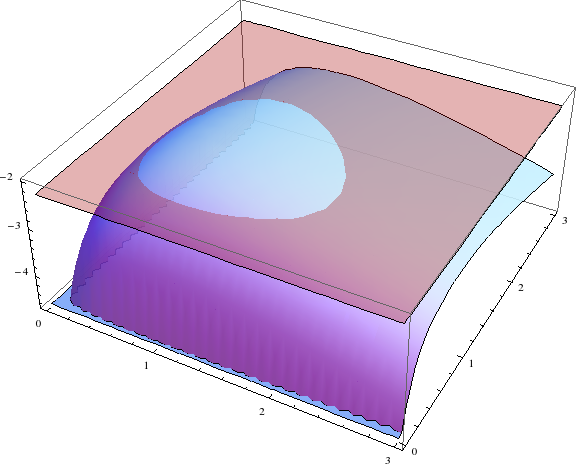
\includegraphics[width=10cm]{images/lotvolsurface.png}
        \caption{\label{lvsur}The function $f$ given by (\ref{lotvolsurface}). Solutions are curves on this surface of constant $C$, i.e. the intersection of the plane $C=\mathrm{const.}$ and the surface $f(x,y)$. Here we see clearly their intersection will always be a closed curve, hence periodic solutions.}
      \end{figure}

      \begin{enumerate}[label=(\alph*)]
        \item We take partial derivatives to first and second order:
          \begin{align}
            &\pd{C}{x}=\gamma\left(\frac{1}{x} - 1\right),\quad   \pd{C}{y}  = \frac{1}{y} - 1,\\
            &\pdd{C}{x} = -\gamma\frac{1}{x^2},\quad  \pdd{C}{y} = -\frac{1}{y^2},\quad \pddmixed{C}{x}{y} = 0.
          \end{align}
          The potential critical points in the surface are at $\pd{C}{x} =\pd{C}{y}=0$ so there is only one possibility, $x=y=1$. The sign of the function
          \begin{equation}
            D = \pdd{C}{y}\pdd{C}{x} - \pddmixed{C}{x}{y}
          \end{equation}
          tells us what kind of critical point we have when $x$ and $y$ take on their critical values:
          \begin{itemize}
            \item $D>0$ and $\pdd{C}{x}<0$: $(x_0,y_0)$ is a maximum,
            \item $D>0$ and $\pdd{C}{x}>0$: $(x_0,y_0)$ is a minimum,
            \item $D<0$: $(x_0,y_0)$ is a saddle point,
            \item $D=0$: indeterminate because $\pd{C}{x}$ and $\pd{C}{y}$ are not linearly independent.
          \end{itemize}
          In our case, $D>0$ and $\pdd{C}{x}<0$ so we have a maximum. As it is the only critical point is a global maximum.

        \item We can think of $C$ as a surface function on the domain $x_0\in[0,\infty]$ and $y_0\in[0,\infty]$ (it is shown in \cref{lvsur} for $\gamma=1$). The solutions $x(t),y(t)$ are curves $\gamma(t)$ on this surface for which $z = C(x_0,y_0)$ is constant: the `height' must be constant. For a given constant $C_0$, a curve (parametrised for a sufficient time period) will be the intersection of the plane $z=C_0$ and the surface of $z = C(x_0,y_0)$. Since the surface has a single global maximum, it looks like a hill, and the intersection of the plane and surface will be a closed curve. A closed curve implies periodicity, but we first must determine that the curve is transversed with a consistent orientation (in a consistent direction around the curve).

          Again dropping back to losing the subscript 0s, we consider the curve as a function of $x$ by solving \cref{lotvolsurface} for $y$ given a value of $C$ and $x$. This gives us a parametrisation for our closed curve $(x,y(x))$. We also remind ourselves that the equations take the form%
          \begin{subequations}%
            \begin{align}%
              \fd{x}{t} &= x(1-y),\\
              \fd{y}{t}&=\gamma y (x-1).
            \end{align}
          \end{subequations}
          There are two points at  which $\fd{x}{t}=0$, for which we have $y=1$. If $\fd{x}{t}$ changes from increasing to decreasing about $\fd{x}{t}=0$ then $y$ must be increasing from $y<1$ to $y>1$, and if  $\fd{x}{t}$ changes from decreasing to increasing about $\fd{x}{t}$, then $y$ must be decreasing from $y>1$ to $y<1$. This gives the curve the same orientation at the two extremes of the curve in the $x$ direction.

          A similar argument for points at which $\fd{y}{t}=0$ (and hence $x=1$) shows the curve is similarly well oriented at both extremes in $y$.

          In between these points we can consider four quadrants, each with varying signs of $\fd{y}{t}$ and $\fd{x}{t}$. For example, let's consider the quadrant $\fd{y}{t}>0$ and $\fd{x}{t}>0$. If we consider travelling in an anti-clockwise direction we enter this section at a point where $\fd{y}{t}=0$ and for which the derivative $\fd{y}{t}$ has changed from decreasing to increasing. In this case $x$ must have increased above $1$ and must stay above $1$ until it reaches the next point where $\fd{y}{t}=0$. Thus the orientation remains consistent on the quadrant $\fd{y}{t}>0$ and $\fd{x}{t}>0$. A similar argument can be applied on all four quadrants to show that the curve $(x,y(x))$ is consistently oriented, and hence the solutions must be periodic. It is easy to see the same argument would apply if the orientation were reversed.

      \end{enumerate}
    }
    %

    %===========================================================================

    %
    \question{Variations on Lotka--Volterra (Exam 2021 \& 2022)}
    {
      \label{graphs-q}
      The graphs on page \pageref{graphs} plot the populations and phase portraits of two species, $x(t)$ and $y(t)$, over time, $t$. Each graph in column \textbf{(G)} has the same initial condition and corresponds to one of the phase portraits in column \textbf{(P)}, and to one of the nondimensionalised models in column \textbf{(M)}. In the models, the constants $\beta,\gamma,\delta>0$ wherever they appear, although they are not necessarily equal between graphs. The rows are numbered \textbf{(1)--(4)}.

      Giving a good reason in each case, match the graphs to the phase portraits and the models. You should not need to find stability: you should be able to connect them by thinking about the models and their meaning alone.

      For example, you could say that \textbf{(G1)} = \textbf{(P2)} = \textbf{(M1)}, if indeed this were correct.
    }
    {
      The matchings (with some example reasonings) are:

      \begin{tabular}{lp{11.5cm}}
        \textbf{(G1)--(P4)--(M3)} & Logistic. Between \textbf{(M3)} and \textbf{(M4)}, \textbf{(M3)} is the only one that allows $y$ to be more than 1, given the initial conditions. For $y>1$, in \textbf{(P4)}, $\fd{y}{t}>0$ in places. This is only possible in \textbf{(M3)} because in \textbf{(M4)}, $\fd{y}{t}<0$ for $y>1$. \\
        \textbf{(G2)--(P3)--(M1)} & Traditional Lotka--Volterra; periodic. \\
        \textbf{(G3)--(P2)--(M4)} & Logistic. Process of elimination. \\
        \textbf{(G4)--(P1)--(M2)} & $\fd{y}{t}$ is always negative. Exponential growth of $x$ once $y$ has decayed exponentially. No equilibrium.
      \end{tabular}
    }
\end{enumerate}

\ifbool{show_question}{
\newpage
\begin{center}
  \label{graphs}
  \textbf{Graphs, phase portraits and models for question \ref{graphs-q}}
\end{center}
\vspace{5mm}

\begin{tabular}{p{0.4cm}p{5cm}p{4.7cm}p{4cm}}
  & \hspace{2.5cm} \textbf{(G)}
  & \hspace{2.5cm} \textbf{(P)}
  & \hspace{1.5cm} \textbf{(M)}\vspace{5mm}\\
  \vspace{-3.2cm}\textbf{(1)} &
  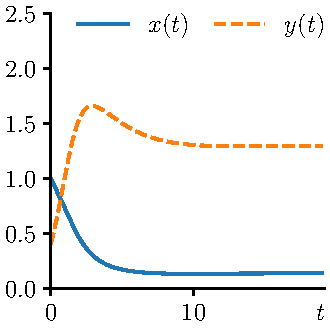
\includegraphics[scale=0.9]{images/graph3a.pdf} &
  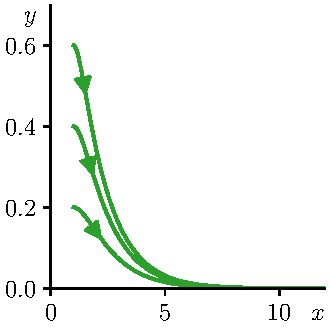
\includegraphics[scale=0.9]{images/graph2b.pdf} &
  \vspace{-3.8cm}$
  \begin{cases}
    \displaystyle\fd{x}{t} = x-xy \vspace{3mm} \\
    \displaystyle\fd{y}{t} = \gamma(-y + xy)
  \end{cases}$
  \\
  \vspace{-3.2cm}\textbf{(2)} &
  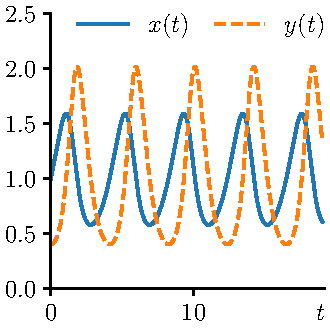
\includegraphics[scale=0.9]{images/graph1a.pdf} &
  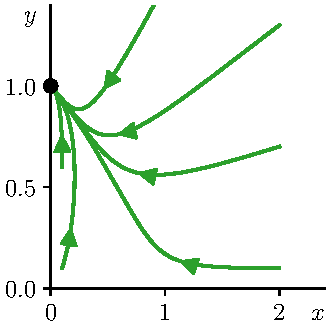
\includegraphics[scale=0.9]{images/graph4b.pdf} &
  \vspace{-3.8cm}$
  \begin{cases}
    \displaystyle\fd{x}{t} = x-xy \vspace{3mm} \\
    \displaystyle\fd{y}{t} = \gamma(-y - xy)
  \end{cases}$
  \\
  \vspace{-3.2cm}\textbf{(3)} &
  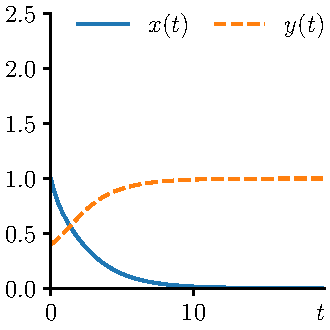
\includegraphics[scale=0.9]{images/graph4a.pdf} &
  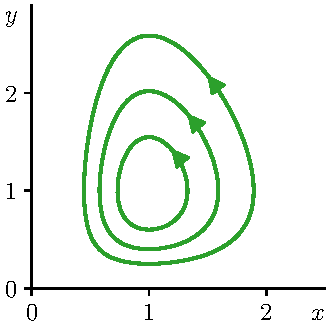
\includegraphics[scale=0.9]{images/graph1b.pdf} &
  \vspace{-3.8cm}$
  \begin{cases}
    \displaystyle\fd{x}{t} = x(1-x) - \gamma xy \vspace{3mm} \\
    \displaystyle\fd{y}{t} = \delta y(1-y) + \beta x y
  \end{cases}$
  \\
  \vspace{-3.2cm}\textbf{(4)} &
  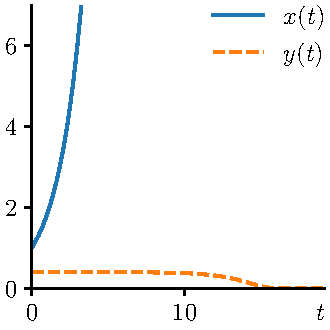
\includegraphics[scale=0.9]{images/graph2a.pdf} &
  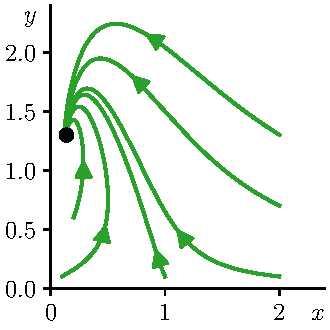
\includegraphics[scale=0.9]{images/graph3b.pdf} &
  \vspace{-3.8cm}$
  \begin{cases}
    \displaystyle\fd{x}{t} = x(1-x) - \gamma xy \vspace{3mm} \\
    \displaystyle\fd{y}{t} = \delta y(1-y) - \beta x y
  \end{cases}$
\end{tabular}
}{}
\end{document}
